\chapterimage{chapter_head_musicalidade.pdf} % Chapter heading image

\chapter{Fundamentos de musicalidade}

\begin{definition}[Musicalidade:] 
\index{Musicalidade}
\label{def:Musicalidade}
A musicalidade pode ser definida como:
\begin{itemize}
\item Particularidade, característica ou estado do que é musical \cite{diciomusicalidade}.
\item Tendência natural, \textbf{sensibilidade} ou talento para criar ou 
tocar música \cite{diciomusicalidade} \cite{merriamwebster-musicalidade}.
\item \textbf{Sensibilidade} para contemplar música; 
\textbf{conhecimento} sobre música \cite{diciomusicalidade}  \cite{merriamwebster-musicalidade}.
\item A \textbf{demonstração do talento} musical de uma pessoa \cite{diciomusicalidade}.
\end{itemize}
\end{definition}





%%%%%%%%%%%%%%%%%%%%%%%%%%%%%%%%%%%%%%%%%%%%%%%%%%%%%%%%%%%%%%%%%%%%%%%%%%%%%%%%
%%%%%%%%%%%%%%%%%%%%%%%%%%%%%%%%%%%%%%%%%%%%%%%%%%%%%%%%%%%%%%%%%%%%%%%%%%%%%%%%
\section{\textcolor{red}{Musicalidade, sentir ou entender a música?}}
Seguindo a Definição \ref{def:Musicalidade}, podemos inferir como entender a musicalidade na dança.
\begin{definition}[Musicalidade na dança:] 
\index{Musicalidade}
\label{def:MusicalidadeNaDanca}
Esta acontece, quando o dançarino tem um estado de ``sensibilidade'' ou ``conhecimento'' para contemplar ou entender a música,
e assim quando este dança, ``demostrar'' uma coerência entre a música e o que está dançando.
\end{definition}

Porem temos um choque de paradigmas, na definição, para atingir um mesmo objetivo que é ser musical.
Podemos \textbf{sentir} ou \textbf{conhecer}; o que é equivalente a dizer que:
\begin{itemize} 
\item podemos saber, por intuição e sensibilidade sem entender porquê, ou
\item podemos saber, entendendo mediante o conhecimento adquirido pelo raciocínio e o estudo da música e sua percepção.
\end{itemize}



Neste sentido, para adquirir esta coerência com a música, 
muitos professores indicam que o dançarino deve ``escutar e sentir a música'';
nesse aspecto, argumento que a frase é metaforicamente correta e coincide em parte com 
as Definições \ref{def:Musicalidade} e \ref{def:MusicalidadeNaDanca};
porem a frase  é pedagogicamente pouco favorável para o estudante.
Assim, eu ressaltaria que a musicalidade a nível de ensino se adquire,
estudando e entendendo a música e como esta é percebida pelo nosso cérebro, e não só sentindo-a.
 
Para fundamentar minha argumentação, acredito interessante expor o Exemplo \ref{ex:srinivasa}. 
\begin{example}[O matemático que sentia os números:]
\label{ex:srinivasa}
Imaginemos que conhecemos ao matemático ``Srinivasa Aiyangar Ramanujan'';
um prodígio matemático autodidata \cite[pp. 1]{kanigel2016man}, indiano, que 
realizou muitas contribuições à matemática\footnote{Existe 
um filme chamado `` The Man Who Knew Infinity'' (2015) ou 
``O Homem que Viu o Infinito'' em português, que conta a história de vida de Srinivasa Aiyangar Ramanujan.}.
E mostramos a ele um problema, % matemático, 
como por exemplo uma equação,
e  lhe pedimos uma resposta ou solução. 
Então Srinivasa, muito amavelmente, 
observaria um instante o problema e nos daria a solução imediatamente.
Nós surpreendidos pela velocidade e o mínimo esforço na resposta,
perguntaríamos: Como você obteve esse resultado? Então ele responderia \cite[pp. 235]{kanigel2016man}: 
%\begin{citando}
%Immediately I heard the problem 
%it was clear that the solution should obviously be a continued fraction; 
%I then thought, Which continued  fraction? And the answer came to my mind.
%\end{citando}
\begin{citando}
No momento em que escutei o problema, 
foi claro pra mim que a resposta devia ser obviamente uma fração continua; 
e então pensei, ¿Qual fração continua? e a resposta chegou a minha mente. 
\end{citando}

Exemplo de fração continua simples:
\begin{equation}
a_{0}+{\frac {1}{a_{1}+{\frac {1}{a_{2}+{\frac {1}{a_{3}+{\frac {1}{\ddots }}}}}}}}
\end{equation}
\end{example}

A resposta que ``Srinivasa'' deu no Exemplo  \ref{ex:srinivasa}, 
é a mesma  que dão as pessoas, quando  dizem que para ter musicalidade ele simplesmente sentiu a música. 
Assim, esta aproximação ao problema é só eficiente, para pessoas como Srinivasa, 
que talvez tenham uma inspiração divina, 
ou que já nasceram com esse dom, ou que por uma longa experiencia de vida atingiram 
a \hyperref[ref:CompetenciaInconsciente]{\textbf{competência inconsciente}}, 
e tem implementado por ``hardware'', no encéfalo, entender a matemática ou a música; 
pelo que eles usam a palavra sentir, 
pois conhecem a resposta, porem não sabem como sabem. 

Assim, este tipo de entendimento  pode acontecer em pessoas que observaram muito tempo um ``problema'', 
ou escutaram muito uma ``música'', 
e um dia conseguiram ``sentir'' a resposta. 
Na minha opinião, 
não todos nascemos com esse componente implementado em nosso encéfalo, para perceber e processar por ``hardware'' (sentir) a música; 
e não podemos nos dar o luxo de escutar uma canção indefinidamente ate ``sentir'' algo. 
O mais eficiente seria estudar música, 
e entender esta baseando-nos em nossa teoria e cruzando esta informação com o que escutamos,
os padrões observados, a melodia, o ritmo, etc. 
Assim, nos podemos criar por ``software'' o que não temos implementado por ``hardware''\footnote{Como no caso do amigo Srinivasa.}, 
derrubando o mito de ``sentir'' a música e passar a ``entender'' ela;
seguindo assim o natural \hyperref[sec:aprendizagem]{\textbf{ciclo da aprendizagem}}\footnote{O
ciclo da aprendizagem é estudado na Seção \ref{sec:aprendizagem}.} passando primeiro pela 
\hyperref[ref:CompetenciaConsciente]{\textbf{competência consciente}} 
antes de atingir a  \hyperref[ref:CompetenciaInconsciente]{\textbf{competência inconsciente}}.

Mas isto não quer dizer que sentir música seja equivocado, é um caminho valido sim;
porem, apontar primeiro a esse alvo, 
pode chegar a ser pouco favorável se temos estudantes baixo nossa responsabilidade,
 que dependem de nós, no seu percorrido para chegar a serem musicais; 
pois se nosso entendimento da musicalidade se baseia unicamente em nossas sensações pessoais,
só poderemos indicar a eles que fechem os olhos e sintam a música.


%%%%%%%%%%%%%%%%%%%%%%%%%%%%%%%%%%%%%%%%%%%%%%%%%%%%%%%%%%%%%%%%%%%%%%%%%%%%%%%%%
\subsection{Musicalidade e teoria da informação}


%% Exemplo dançar em coerencia com a música ou não
%% Eurythmics - Sweet Dreams (Are Made Of This) (Official Video)

Dançar com musicalidade não é só dançar com o \hyperref[ref:Pulso]{\textbf{pulso}} da música, 
ou na \hyperref[def:Metrica]{\textbf{métrica}},
existem outros aspectos da música, ou de instrumentos isolados, que podemos seguir como 
\begin{inparaitem} 
\item a melodia, 
\item o ritmo,
\item a \hyperref[sub:Articulation]{\textbf{articulação}} das notas, 
\item as \hyperref[sec:texturasmusica]{\textbf{texturas}}, 
\item as \hyperref[sec:Cadencia]{\textbf{cadências}}, 
\item os \hyperref[sec:Motivo]{\textbf{motivos}}, 
\item o \hyperref[sec:fraseio]{\textbf{fraseio}}, 
\item etc.
\end{inparaitem} 
Com todos esses fatores, uma pessoa com musicalidade, 
pode incorporar as caraterísticas que considere que sejam interessantes para 
ser mostradas na sua dança; como por exemplo, poderíamos dançar interpretando a letra da música.

Neste ponto chegamos a uma pregunta; se eu danço usando a letra e faço exatamente o oposto,
estou dançando com musicalidade?
Para poder responder isto, confiantes na nossa afirmação,
primeiro teríamos que nos fazer outra pergunta.
Se eu danço fazendo o oposto de uma caraterística da música que tenho escolhido,
minha dança seria uma função direta dessa caraterística?
Neste caso a resposta seria ``sim'', pois mesmo fazendo o oposto,
nossa dança estaria atrelada à caraterística escolhida na música.
Pelo que podemos afirmar que se dançamos fazendo o oposto a uma caraterística da música, 
estamos sim dançando com musicalidade.
\begin{example}[A criança não-independente:]
Imaginemos que temos baixo nossa responsabilidade a uma criança,
e esta precisa ir a dormir cedo, pelo que lhe indicamos a ela que já deve ir a dormir;
se a criança é obediente vai a dormir, então seus atos estariam em função de nossos comandos,
pelo que poderíamos considerar ela como dependente de nós;
porem se a criança é ``falsamente'' independente (falsamente rebelde), quando indiquemos que deve ir a dormir,
por contradição ela ficará acordada, mesmo sentindo sono, por ter um falso senso de independência.

Nesse caso a criança é dependente de nossas ordens,
pois seus atos estão em função direta do que nos indiquemos.
Um individuo realmente independente, tomaria suas decisões unicamente em função,
do seu próprio analises e conclusões.
Pelo que poderíamos afirmar que no caso da criança falsamente rebelde, esta é dependente da autoridade.
\end{example}

É neste ponto que podemos invocar à ``teoria da informação'' para que nós possamos explicar,
ou modelar, esta dependência entre nossos movimentos e a música.
Nesta área do conhecimento existem duas definições, que são:
\begin{itemize} 
\item A informação mútua (binária), que mede a informação que tem em comum dois eventos ou variáveis,
sendo 1.0 quando ambas tem completamente a mesma informação,
zero quando ambas variáveis não tem informação em comum, 
e valores intermediários entre zero e 1.0 quando existe entre eles uma porção da informação \cite{reza2012introduction}. 
\item O coeficiente de correlação (Pearson), 
que indica o grau de dependência a favor ou em contra entre dois eventos ou variáveis,
sendo +1.0 quando os eventos crescem juntos, 
-1.0 quando um cresce enquanto u outro diminui na mesma proporção,
 zero quando os dois eventos não tem nada em comum, 
e valores intermediários entre -1.0 e +1.0 para graus intermediários de correlação \cite{reza2012introduction}.
\end{itemize} 

Note-se que a informação mútua entre duas variáveis só tem sinal positiva; assim,
se uma variável cresce na mesma proporção que outra diminui, 
a informação mutua será 1.0 pois uma variável é completamente dependente da outra
\begin{example}
Dadas as variáveis  $X$ e $Y$, se $Y=-X+3$; então,
a informação mutua entre X e Y é igual a $1.0$, e
a correlação entre $X$ e $Y$ é igual a $-1.0$.
\end{example}

Das explicações anteriores podemos deduzir que: as relações entre a música e a dança, 
são melhor descritas com a informação mutua  que com a correlação;
pelo que podemos reformular a Definição \ref{def:MusicalidadeNaDanca} usando a informação mutua:
\begin{definition}[Musicalidade na dança seguindo a teoria da informação:] 
\index{Musicalidade}
\label{def:MusicalidadeNaDancaIT}
A musicalidade é um termo que indica o grau de informação mutua que existe entre dois eventos: 
\begin{itemize}
\item A música que é percebida.
\item Os movimentos que são executados.
\end{itemize} 
\end{definition}


Se definimos a $M_u$ como uma variável que representa a informação da música, e 
a $M_o$ como uma variável que representa a informação dos movimentos, 
como mostrado na Figura \ref{fig:InfoMutuaMuMo}.
\begin{figure}[!h]
  \centering
    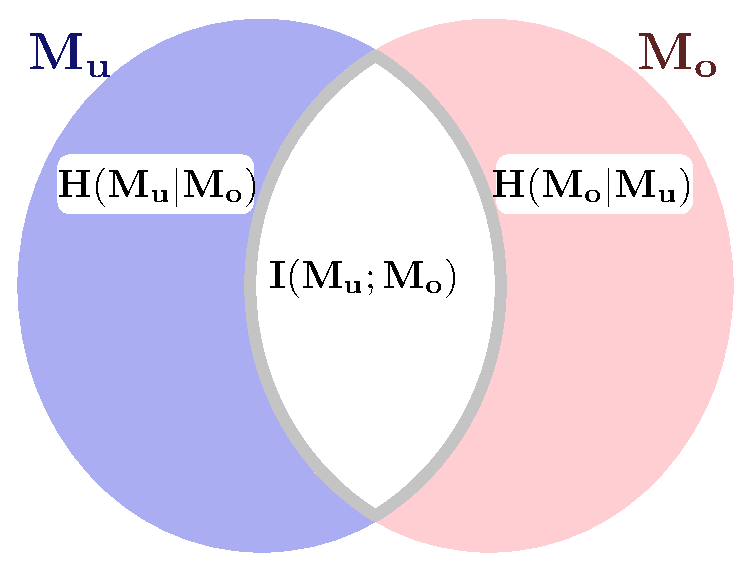
\includegraphics[width=0.35\textwidth]{chapters/cap-musicalidade/musicalidade-it.eps}
\caption{Informação mutua entre $M_u$ e $M_o$.}
\label{fig:InfoMutuaMuMo}
\end{figure}

Então seguindo a Definição \ref{def:MusicalidadeNaDancaIT},
podemos afirmar que:
\begin{itemize}
\item $\mathbf{I(M_u;M_o):}$ é a informação mutua entre a música ($M_u$) e os movimentos ($M_o$),
e representa a quantidade de musicalidade na dança.
\item $\mathbf{H(M_u|M_o):}$ é a informação que tem a música que não tem os movimentos.
Por exemplo, quando dançamos e a música está simplesmente de fundo, 
só sendo um elemento que emoldura os nossos movimentos sem afetar-lhos diretamente,
então teremos um caso de música incidental\footnote{A música incidental é muito utilizada no cinema, 
teatro, TV e video games; nestes âmbitos existe uma música de fundo que cria um ambiente para a cena \cite[pp. 17]{reinato2010musica} \cite[pp. 217]{dourado2004dicionario},
onde pouca informação da musica está sendo usada, e esta serve só de marco emocional ou entrega uma informação além da ação na cena, para o espectador.}, e a informação musical não usada seria $H(M_u|M_o)$.
\item $\mathbf{H(M_o|M_u):}$ é a informação que tem os movimentos que não tem a música.
Por exemplo, se temos música incidental de caráter melancólica, e iniciamos a 
realizar movimentos em sequencia que representam a historia de nossa vida;
então a informação de nossa vida seria  $H(M_o|M_u)$.
\end{itemize}~

Finalmente, é interessante propor a seguinte pergunta e reflexão,
qual das danças mostradas na Figura \ref{fig:ex:infomutua} consideras com musicalidade?


\begin{figure}[ht]
\centering
\begin{subfigure}{.42\textwidth}
  \centering
  % include first image
  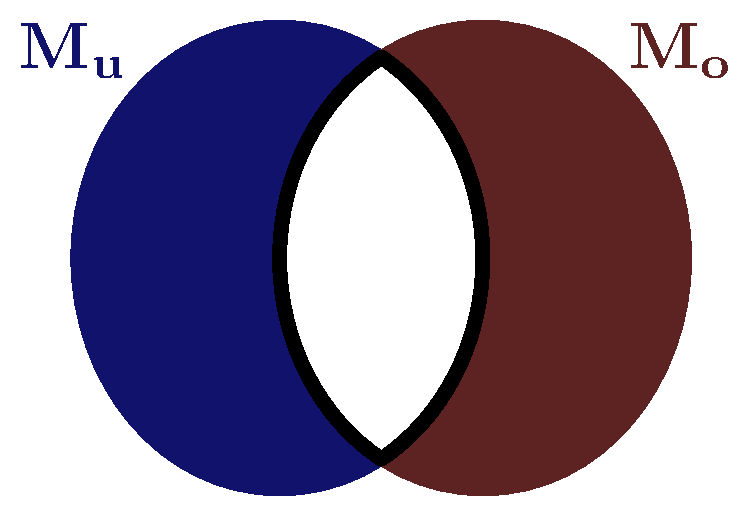
\includegraphics[width=.9\linewidth]{chapters/cap-musicalidade/musicalidade-it1.eps}  
  \caption{Caso 1.}
  \label{fig:ex:infomutua:a}
\end{subfigure}
\hfill	
\begin{subfigure}{.28\textwidth}
  \centering
  % include second image
  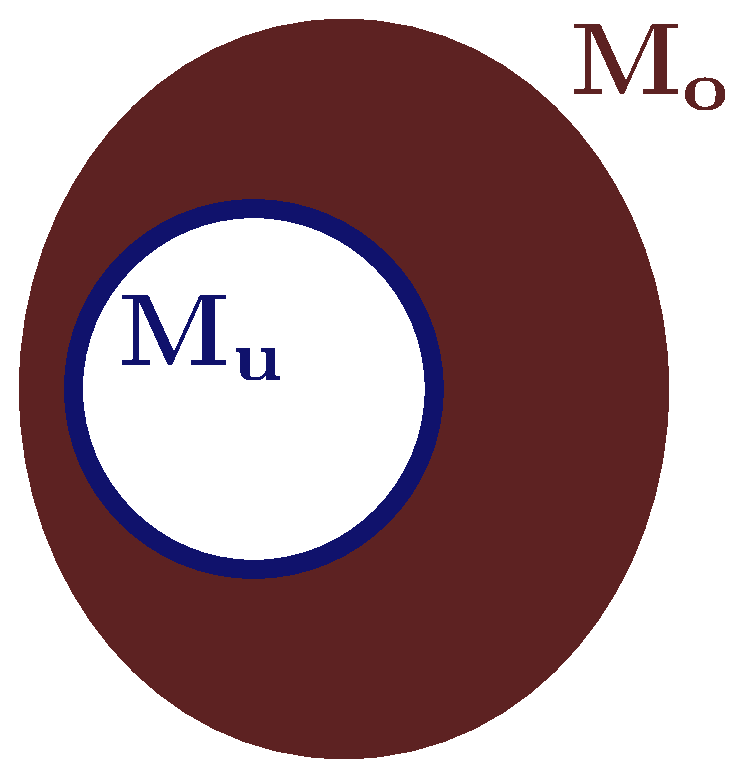
\includegraphics[width=.9\linewidth]{chapters/cap-musicalidade/musicalidade-it2.eps}  
  \caption{Caso 2.}
  \label{fig:ex:infomutua:b}
\end{subfigure}
\hfill
\begin{subfigure}{.28\textwidth}
  \centering
  % include second image
  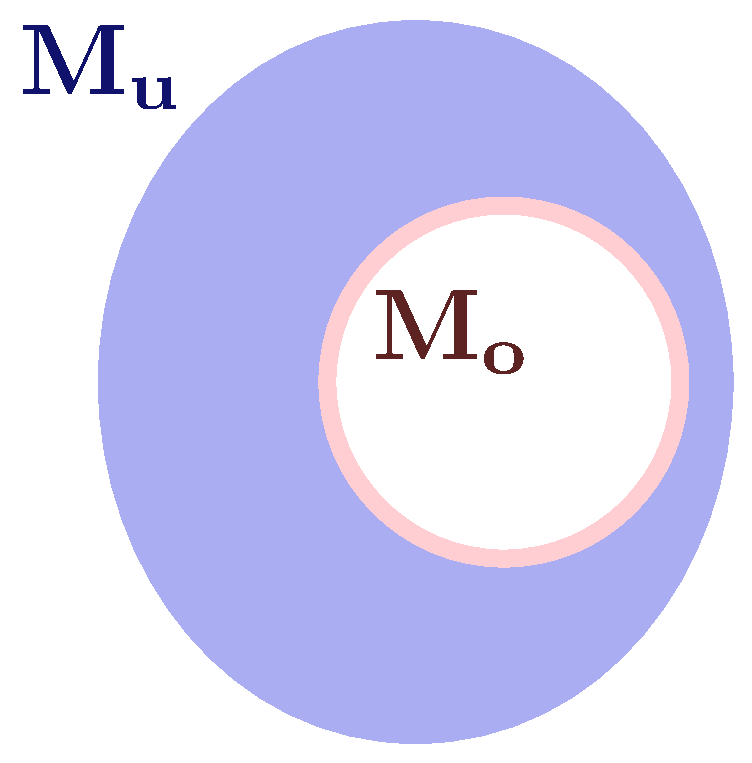
\includegraphics[width=.9\linewidth]{chapters/cap-musicalidade/musicalidade-it3.eps}  
  \caption{Caso 3.}
  \label{fig:ex:infomutua:c}
\end{subfigure}
\hfill
\begin{subfigure}{.52\textwidth}
  \centering
  % include first image
  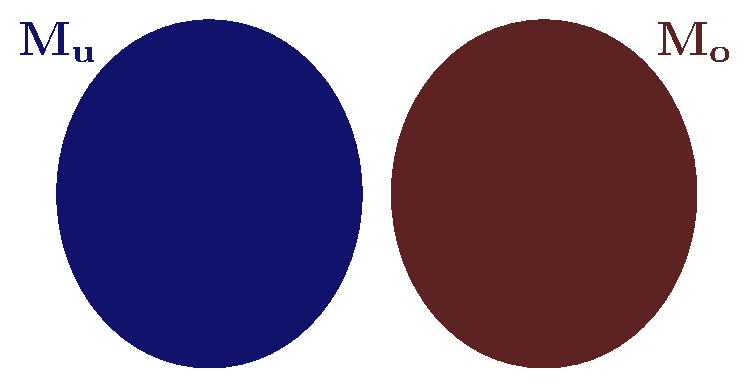
\includegraphics[width=.9\linewidth]{chapters/cap-musicalidade/musicalidade-type3.eps}  
  \caption{Caso 4.}
  \label{fig:ex:infomutua:d}
\end{subfigure}
\caption{Distintos tipos de usos da música na dança.}
\label{fig:ex:infomutua}
\end{figure}

Pessoalmente, eu me imagino:
\begin{itemize}
\item Na Figura \ref{fig:ex:infomutua:a} a um casal amigo meu dançando felizes.
\item Na Figura \ref{fig:ex:infomutua:b} escuto uma melodia simples, um solo de flauta,
fazendo em bucle uma frase de 4 compassos, 
e nessa música uma moça contando mediante a dança a historia da sua vida.
\item Na Figura \ref{fig:ex:infomutua:c} escuto uma musica complexíssima, 
provavelmente polifônica, e um rapaz fazendo popping-dance,
onde cada um do seus movimento está atrelado às vontades de um instrumento na música.
\item Na Figura \ref{fig:ex:infomutua:d} me imagino a uma pessoa dançando de forma descompromissada com a música.
\end{itemize}


%%%%%%%%%%%%%%%%%%%%%%%%%%%%%%%%%%%%%%%%%%%%%%%%%%%%%%%%%%%%%%%%%%%%%%%%%%%%%%%%%
\begin{comment}
\subsection{\textcolor{red}{Relações da música com a dança}}
Em relação a como nossos movimentos são encaixados ou atrelados à música,
podem existir  3 tipos de relacionamento:
dependente, interdependente e independente \cite{butterworth2011dance}.

\begin{description}
\item[Dependente:] Este conceito de relação de dependência, entre musica e dança, pode ter pelo menos 3 acepções.
\begin{description}
\item[Mickey mousing:]
\item[visualização musical:]
\item[Correlação direta:]
\end{description}
\item[Interdependente:] Este é um termo usado para designar uma relação amigável,
entre música e dança; é dizer quando a música da um contexto onde se emoldura a dança,
porem esta tem liberdade de improvisar e contar historias dentro de uma estrutura definida, 
e usa a música como marco emocional e guia;
também pode-se referir ao caso quando, entre música e dança, 
se da uma relação de trabalho de pergunta e resposta, em ambos sentidos \cite{butterworth2011dance}. 
Este tipo de relação com a música está bem descrita pela Figura \ref{fig:ex:infomutua:a}.
\item[Indefinidamente:]
\end{description}
\end{comment}

%%%%%%%%%%%%%%%%%%%%%%%%%%%%%%%%%%%%%%%%%%%%%%%%%%%%%%%%%%%%%%%%%%%%%%%%%%%%%%%%
% https://translate.google.com.br/translate?sl=en&tl=pt&u=https%3A%2F%2Fthisdancinglife.com%2Fmusicality-in-dance%2F

%%%%%%%%%%%%%%%%%%%%%%%%%%%%%%%%%%%%%%%%%%%%%%%%%%%%%%%%%%%%%%%%%%%%%%%%%%%%%%%%
\section{\textcolor{blue}{Interpretação corporal da música}}


\begin{comment}
\begin{figure}[t]
\begin{elaboracion}[title=Que é o ``flow''?]
\label{page:flow}
\index{Musicalidade!Flow}
\textcolor{red}{Nós nos perdemos no movimento e na música,
esquecendo as restrições do tempo e da normalidade, este fenomeno é conhecido como ``Flow''} \cite{czikszentmihalyi1990flow} \cite{trehub2003developmental}.
\end{elaboracion}
\label{fig:flow}
\end{figure}
\end{comment}

Seguindo a Definição \ref{def:MusicalidadeNaDanca},
para que um dançarino tenha musicalidade, este precisa primeiro,
incorporar em si mesmo a informação que traz a música, 
este processo é chamado de \hyperref[cap:percepcaomusical]{\textbf{percepção musical}}, 
e ja foi abordado no Capítulo \ref{cap:percepcaomusical}.
Com esta informação, o dançarino deve procesar e escolher uma forma de interpretar corporalmente,
esta informação, ver Figura \ref{fig:interpretacion-corporal}.
\begin{figure}[!h]
  \centering
    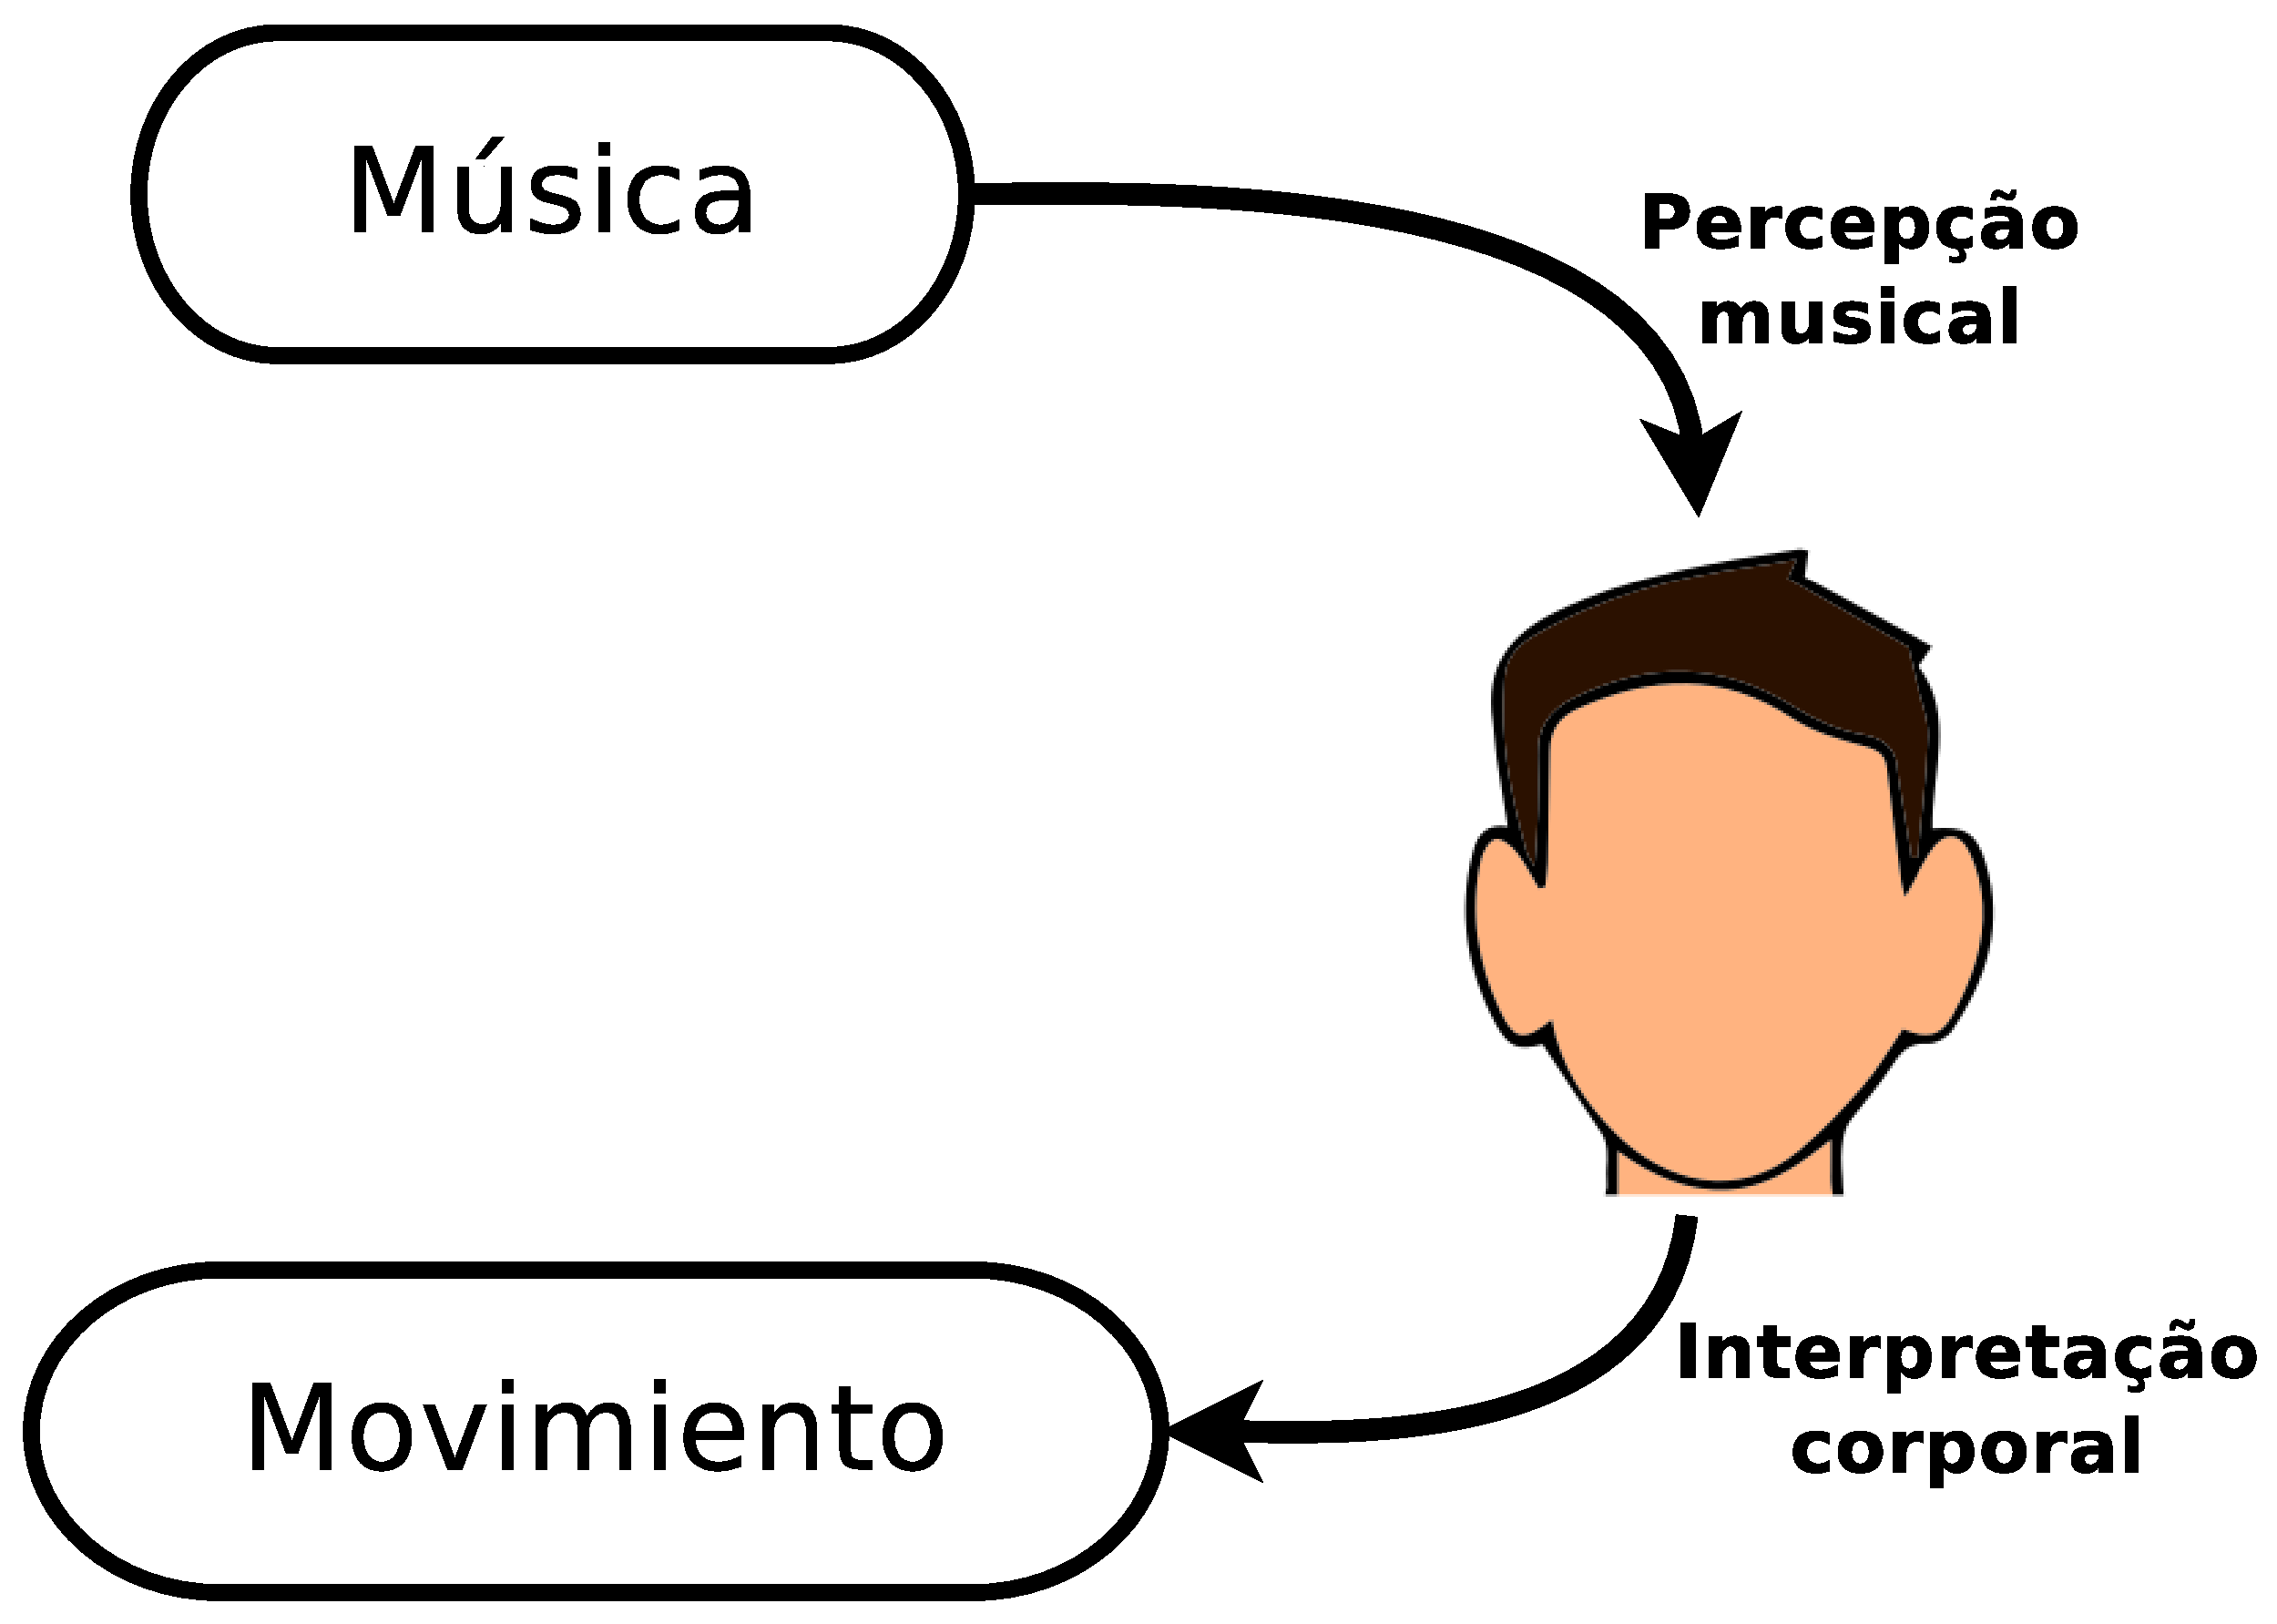
\includegraphics[width=1.00\textwidth]{chapters/cap-musicalidade/interpretacion-corporal.eps}
\caption{Interpretação corporal da música.}
\label{fig:interpretacion-corporal}
\end{figure}


\textcolor{red}{ver Figura \ref{fig:mapeamento}}.
\begin{figure}[!h]
  \centering
    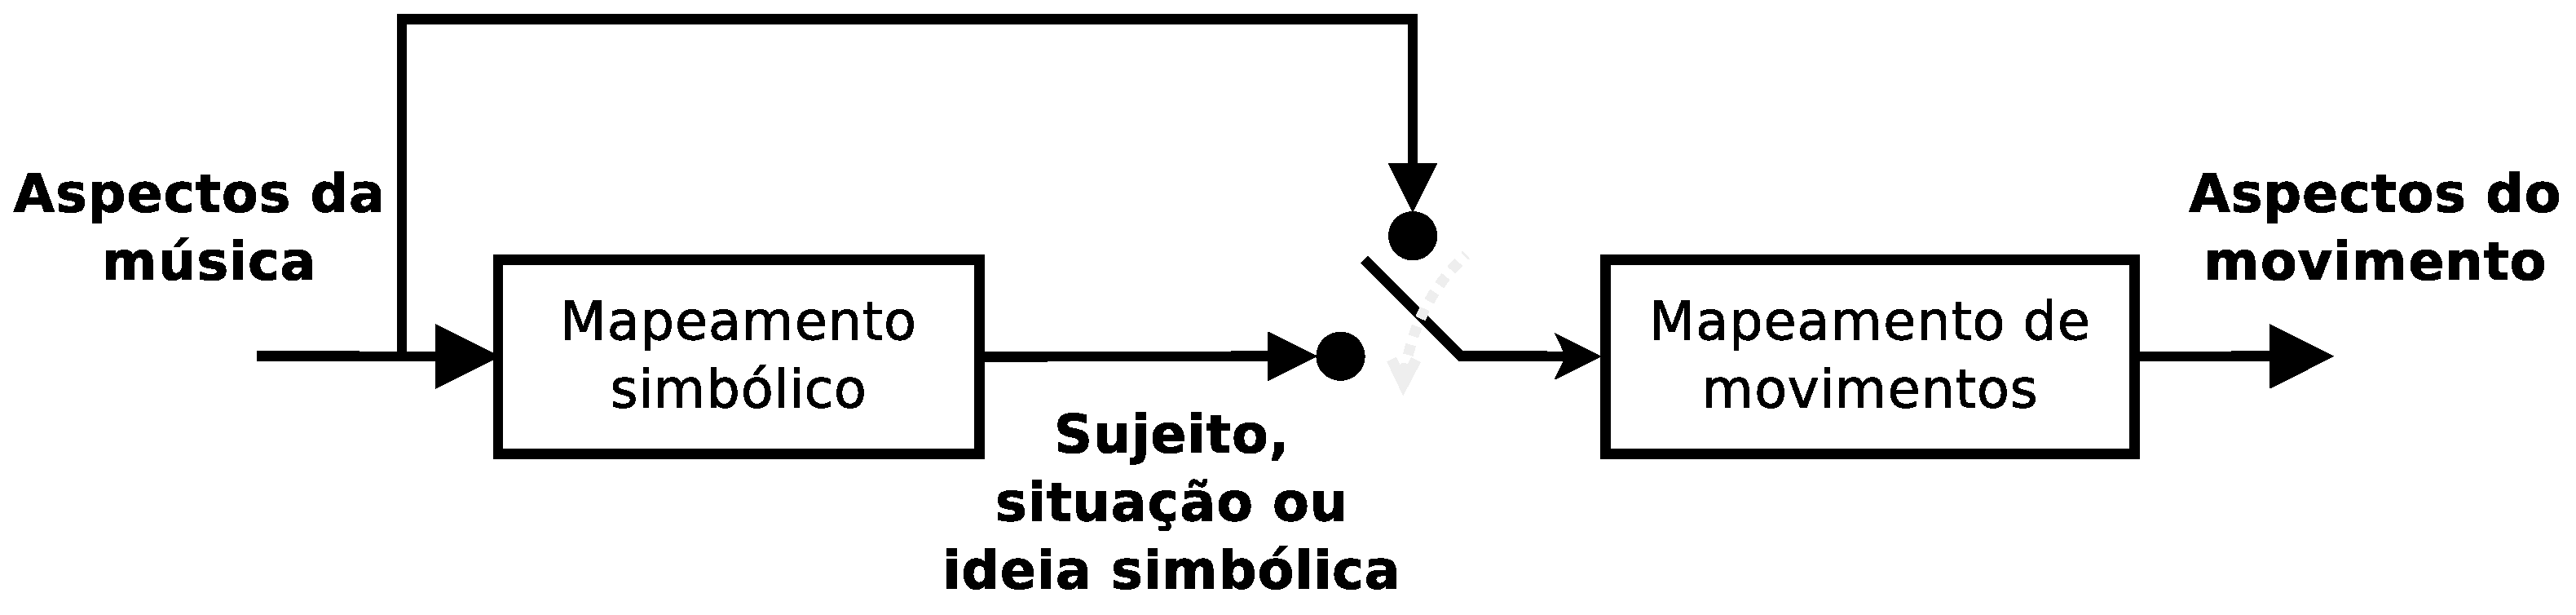
\includegraphics[width=1.00\textwidth]{chapters/cap-musicalidade/mapeamento.eps}
\caption{Mapeamento de ideias e estimulos a movimentos.}
\label{fig:mapeamento}
\end{figure}


As formas de como o dançarino interpreta esta informação estão amplamente estudadas,
não só no âmbito da dança, se não de forma geral no âmbito das artes cênicas;
entre os pontos de estudo, mais difundidos, 
para a interpretação de ideias  mediante o uso do corpo, podemos encontrar:
\begin{itemize}
\item A consciência corporal,
\item o controle corporal,
\item a dissociação corporal, e
\item a expressão corporal.
\end{itemize}
Para conhecer as definições e mais detalhes de como podemos aprimorar estes tópicos,
invito aos leitores a ir ao capítulo \ref{fig:bodyrelations}.

No caso da dança a dois, o dançarino usa todos estes elementos, 
para enviar ou projetar corporalmente uma informação, que tenha coerência com a música que percebe.
Os receptores ou destinatários destas informações, podem ser: o par de dança,
o público, ou o próprio dançarino; 
assim, dependendo do âmbito em que este se desenvolva,
podem incluso ser todos eles, ao mesmo tempo, os receptores da informação.

É neste ponto que o dançarino tem mais liberdade criativa, 
e onde podem ser introduzidas subjetividades; por exemplo,
se a ideia ou informação recopilada pelo dançarino está representada pela Figura \ref{fig:LaCopaDeRubin};
este interpretará um  movimento de bêbados ou de namorados?
\begin{figure}[!h]
  \centering
    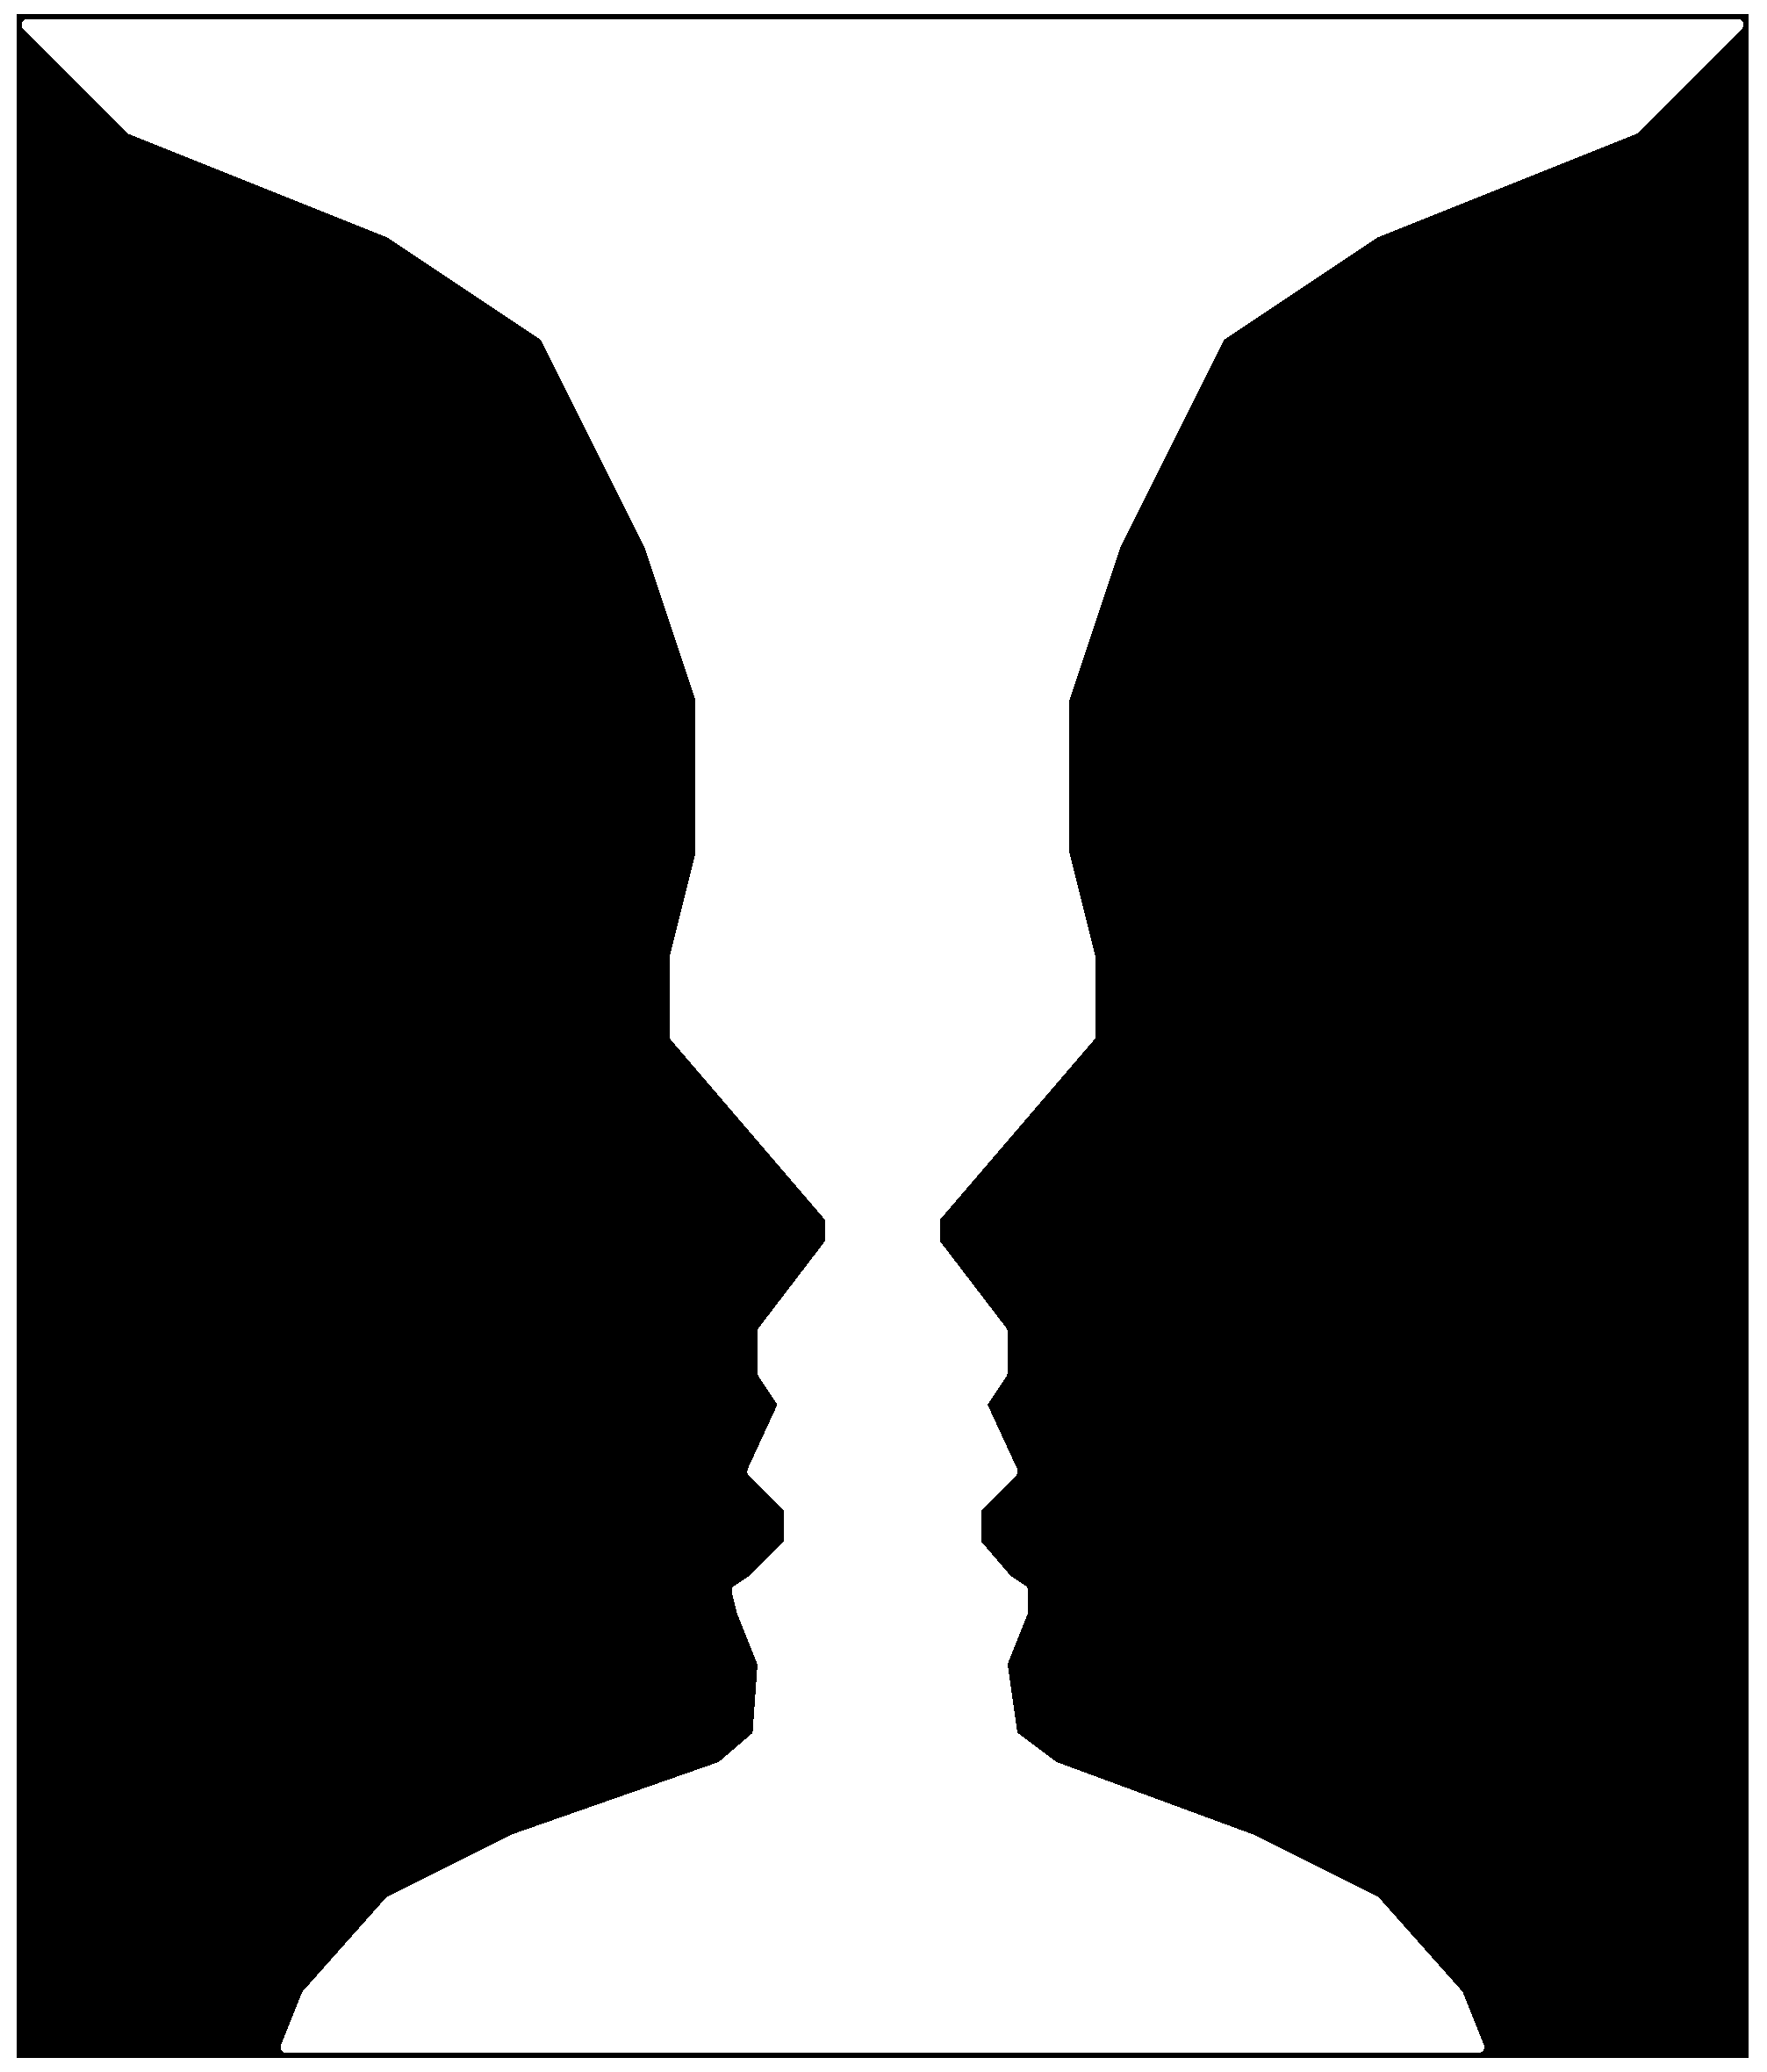
\includegraphics[width=0.5\textwidth]{chapters/cap-musicalidade/LaCopaDeRubin.eps}
\caption{Aperspetiva do interprete.}
\label{fig:LaCopaDeRubin}
\end{figure}

O objetivo deste capítulo e dos seguintes, não é indicar se na Figura \ref{fig:LaCopaDeRubin},
existe uma copa ou duas pessoas se olhando frente a frente; e sim desenvolver técnicas ou 
apresentar treinamentos para projetar qualquer destas duas perspetivas, seguindo a interpretação de cada dançarino.




%%%%%%%%%%%%%%%%%%%%%%%%%%%%%%%%%%%%%%%%%%%%%%%%%%%%%%%%%%%%%%%%%%%%%%%%%%%%%%%%
%%%%%%%%%%%%%%%%%%%%%%%%%%%%%%%%%%%%%%%%%%%%%%%%%%%%%%%%%%%%%%%%%%%%%%%%%%%%%%%%
\section{Contagens dos passos para o ensino}
Antes de iniciar esta seção é importante mencionar uma
problemática que é vista com muita frequência nas escolas de dança; 
esta é gerada a consequência de que entre os profissionais da música e os da dança
existe uma diferença entre a forma em que os tempos são contados na música. 
Em geral a contagem dos profissionais da música segue a \hyperref[def:Metrica]{\textbf{métrica}}
e no caso dos profissionais da dança segue, em varias ocasiões, 
um enfoque particular a cada escola de dança, 
visando só em muitos casos 
o fácil entendimento do aluno na execução do movimento programado para a aula do dia, 
sem procurar uma rigorosidade teórica no uso de termos e expressões musicais.



%%%%%%%%%%%%%%%%%%%%%%%%%%%%%%%%%%%%%%%%%%%%%%%%%%%%%%%%%%%%%%%%%%%%%%%%%%%%%%%%
\subsection{Contagem de 3 passos em 2 tempos}
\label{susec:3passos2tempos}
A diferença\footnote{Na Pag. \pageref{fig:RitmoVsFala} podemos ver uma explicação
acerca das diferenças na percepção de um ouvinte
sobre o inicio e o final de um ritmo.} 
entre
% 
a subjetiva percepção auditiva que podemos ter acerca do tempo de inicio de um padrão rítmico e 
o verdadeiro tempo musical em que este padrão inicia dentro  de um \hyperref[def:Compasso]{\textbf{compasso}}, 
%
leva a um problema quando se quer ser rigoroso na forma de contar os tempos dos movimentos na dança; 
por exemplo, na Tabela \ref{tab:ritmo1} podemos ver 5 formas distintas que as pessoas usam 
para contar os ``tempos'' nos compassos. 
Nesta tabela a variável ``$T$'' representa um tempo do compasso (\hyperref[subsec:compassobinario]{\textbf{binário}}).
\begin{table}[h]
  \centering
  \begin{tabular}    {c|ccc|c}
    \hline
    Tipos de contagem       & $T/2$ & $T/2$   & $T$ (Forte) & Recomendável?\\
    \hline
    Contagem 1: & tchic  & tchic  & tum   & Sim\\
    Contagem 2: & 2     & e     & 1     & Sim\\ \hline
    Contagem 3: & Con   & tra  & Tempo & Não\\
    Contagem 4: & 1     & e     & 2     & Não\\  \hline
    Contagem 5: & 1     & 2     & 3     & Depende\\ \hline
    \hline
  \end{tabular}
  \caption{Tipos de contagem na samba de gafieira.}
\label{tab:ritmo1}
\end{table}

As formas de contagem que recomendo são:
\begin{itemize}
\item \textbf{A contagem 1}, 
isto é devido a que pode ser usada sem aprofundar demasiado 
na notação musical, a nível de ensino só precisa ser explicado que a duração de um 
``tum'' é o dobro que um ``tchic'' e indicar que tipicamente veremos que o ``tum''
acontece no tempo 1 (forte) do compasso.
%de modo que outra contagem valida seria ``tum tchic tchic''; 

A contagem 1 não está restrita ao uso destas silabas (``tchic'' e ``tum''), 
em geral esta contagem representa a qualquer padrão de repetição
que use duas silabas diferentes, como por exemplo os padrões: ``ta-ta kum'', ``tic-tic kum'', etc. 
Este tipo de contagem já é usada na prática e na literatura sobre dança, pois 
podemos achar variantes como ``quick-quick slow'' (rápido-rápido lento no idioma inglês)
ou ``tic-tic tum'' seguindo a notação usada por Perna no seu livro sobre samba de gafieira \cite[pp. 146]{perna2002samba}.
\item \textbf{A contagem 2}, segue a notação da contagem dos tempos no compasso, esta
contagem é coerente com a música, porém precisa de uma explicação  
para pessoas não iniciadas na notação musical; isto não quer dizer que seu
entendimento seja complexo e sim que precisa um investimento em minutos de aula
um pouco major que a contagem 1.
Mesmo assim, devemos ter cuidado pois pode-se dar o caso que a partitura não tenha compassos binários 
e sim quaternários (com tempos de 1 até 4), 
criando a contagem 2 mais caminhos onde podemos perder coerência com a contagem que segue a métrica.
\end{itemize}


Entre as contagens que não recomendo estão:
\begin{itemize}
\item \textbf{A contagem 3} (``con-tra tempo''), 
devido a que o uso deste padrão pode confundir às pessoas que desconhecem 
a definição (musical) do termo \hyperref[sec:contratempo]{\textbf{contratempo}} 
\cite[pp. 16]{mascarenhascurso} \cite[pp. 36]{azevedocompor}, 
levando à confusão de achar que um contratempo é só uma distribuição de 3 tempos, 
sendo um o dobro dos outros dois, em termos de tempos execução.
\item \textbf{A contagem 4} não é recomendada devido a que como é visto nas Figuras 
\ref{fig:abc-caquarela} e \ref{fig:abc-tchic-tchic-tum-1}, musicalmente a contagem estaria invertida,
dado que o tempo 1 do compasso corresponde ao tempo forte.
\end{itemize}~

Finalmente, a contagem que precisa um cuidado especial:
\begin{itemize}

\item \textbf{A contagem 5} precisa ser bem explicada, 
devido a que não segue a notação musical; 
porém, seu uso é didático e pode ser resgatado se fazemos em todo instante a aclaração de 
que se trata de uma contagem de \hyperref[sec:TemposCoreograficos]{\textbf{tempos coreográficos}}.
Assim, ficará claro para o estudante, 
que esta contagem não corresponde necessariamente com os tempos musicais, 
que também devem ser ensinados.
Para mais detalhes sobre os tempos coreográficos ver a Seção \ref{sec:TemposCoreograficos}.

%não é recomendada, 
%por motivos similares aos apresentados para a contagem 4. 
%Além do fato que os números atribuídos estão distantes da
%notação verdadeira na partitura, mesmo sim esta houvesse sido escrita num compasso quaternário.
\end{itemize}


%%%%%%%%%%%%%%%%%%%%%%%%%%%%%%%%%%%%%%%%%%%%%%%%%%%%%%%%%%%%%%%%%%%%%%%%%%%%%%%%
\subsection{Contagem de 2 passos em 2 tempos}

Na Tabela \ref{tab:ritmoconta2}  podemos ver 5 formas distintas que as pessoas adotam 
para contar dois passos em dois tempos nos \hyperref[subsec:compassobinario]{\textbf{compassos binários}}.
Na tabela se indica a distribuição de tempos na qual ``$T$'' representa um tempo do compasso.

\begin{table}[ht]
  \centering
  \begin{tabular}    {c|cc|c}
    \hline
    Tipos de contagem       & $T$ (fraco)  & $T$ (Forte)& Recomendável?\\
    \hline
    Contagem 1: & tum  & TUM  & Sim\\
    Contagem 2: & 2     & 1     & Sim\\
    Contagem 3: & tempo & Tempo & Sim\\ \hline
    Contagem 4: & 1     & 2     & Não\\ \hline
    Contagem 5: & 1     & 3     & Depende\\  \hline
    \hline
  \end{tabular}
  \caption{Tipos de contagem na samba de gafieira.}
\label{tab:ritmoconta2}
\end{table}



As formas de contagem que recomendo são:
\begin{itemize}
\item \textbf{A contagem 1}, pode ser usada sem aprofundar demasiado 
na notação musical, na qual só precisa ser explicado que cada onomatopeia ``tum'' tem a mesma duração,
de modo que  o ``tum'' que cai no tempo 1 será falado com maior intensidade (``TUM'').
\item \textbf{A contagem 2}, segue a mesma ideia que a contagem 1, 
com a diferencia de que aqui são usados os números dos tempos nos compassos binários.
\item \textbf{A contagem 3} 
é similar a contagem 1, 
com a diferença de que em vez de contar usando a onomatopeia ``tum'',
usamos a palavra ``tempo'' para ressaltar que cada um deles dura um tempo do compasso. 
\end{itemize}~

A forma de contagem que não recomendo é:
\begin{itemize}
\item \textbf{A contagem 4}, pois está invertida em relação a contagem que segue a 
\hyperref[def:Metrica]{\textbf{métrica}} dos \hyperref[subsec:compassobinario]{\textbf{compassos binários}},
pelo que pode trazer confusões.
\end{itemize}~

Finalmente, a contagem que precisa um cuidado especial:
\begin{itemize}
\item \textbf{A contagem 5} precisa ser bem explicada 
devido a que não segue a notação musical. 
Esta é uma consequência da contagem ``1,2,3'' vista na Seção \ref{susec:3passos2tempos}, 
seu uso é didático e pode ser usada se fazemos em todo momento a indicação de 
que se trata de \hyperref[sec:TemposCoreograficos]{\textbf{tempos coreográficos}},
de este modo ficará claro para o estudante que esta contagem não usa os tempos da música.
%Para mais detalhes sobre os tempos coreográficos ver a Seção \ref{sec:TemposCoreograficos}.
\end{itemize}






%%%%%%%%%%%%%%%%%%%%%%%%%%%%%%%%%%%%%%%%%%%%%%%%%%%%%%%%%%%%%%%%%%%%%%%%%%%%%%%%
%%%%%%%%%%%%%%%%%%%%%%%%%%%%%%%%%%%%%%%%%%%%%%%%%%%%%%%%%%%%%%%%%%%%%%%%%%%%%%%%
\section{Contagem de tempos correográficos}
\label{sec:TemposCoreograficos}
\index{Musicalidade!Tempos coreográficos}
Nesta seção presentamos e definimos o conceito de ``tempo coreográfico''.
Quando criamos uma coreografia (grupo de movimentos), 
definimos para esta uma distribuição de tempos em que os movimentos serão executados.
Para conseguir isto, usamos como unidade de medida um tempo de referencia,
de modo que cada movimento do grupo tem sua duração em função deste tempo.
\begin{definition}[Tempo coreográfico:] 
\label{def:tempocoreografico}
é a unidade de medida básica, com que os movimentos de uma coreografia são ordenados e distribuídos.
Um tempo coreográfico não precisa ter uma representação em segundos,
este dado só será relevante quando a coreografia seja encaixada numa música;
nesse caso: 
\begin{itemize}
\item Deverá ser indicada a equivalência entre os tempos coreográficos e musicais.
\item Também, deverá ser indicado a posição do primeiro tempo coreográfico em relação aos tempos musicais.
\end{itemize}
\end{definition}
Assim, a principio, os tempos coregráficos são bastante livres, 
e seu uso e criação depende exclusivamente da imaginação do coreografo.


Para evitar confusões na leitura, usaremos a abreviatura ``TC'' 
antes do número que indica o tempo coreográfico,
para diferenciar este da contagem do tempo musical,
de modo que quatro tempos coreográficos em sequência seriam escritos como: 
\{TC1, TC2, TC3, TC4\}.

De forma similar, para indicar um conjunto de 4 movimentos, 
sugerimos utilizar a abreviatura ``M''; de modo que quatro movimentos de uma coreografia,
ordenados em sequência seriam escritos como: 
\{M1, M2, M3, M4\}.

\begin{example}
Imaginemos que estamos criando o movimento chamado \hyperref[subsec:passo:romario]{\textbf{Romário}},
e decidimos iniciar ele da postura de X; percebemos então que faremos 6 movimentos,
de modo que o terceiro e sexto tem o tempo de espera dobrado, 
em relação aos demais movimentos que tem o mesmo tempo de espera apos serem executados.

Assim para descrever o Romário, antes de ser incrustado na música, 
poderíamos usar a seguinte sequencia de tempos coreográficos: \{TC1, TC2, TC3, TC5, TC6, TC7\},
que correspondem aos movimentos \{M1, M2, M3, M4, M5, M6\} da coreografia, respetivamente.

Para incrustar esta coreografia na música, o único que precisamos indicar,
é que a coreografia inicia no tempo 2 do compasso (tempo fraco)
e que cada tempo coreográfico dura meio tempo musical.

A contagem de tempos coreográficos pode ser vista na primeira linha de texto na pauta mostrada na Figura \ref{fig:contagemtempocoreografico};
na segunda linha de texto da pauta podemos ver a contagem dos tempos musicais,
onde vemos que o movimento todo da coreografia dura 4 tempos musicais.
\end{example}

\begin{figure}[!h]
    \centering
    %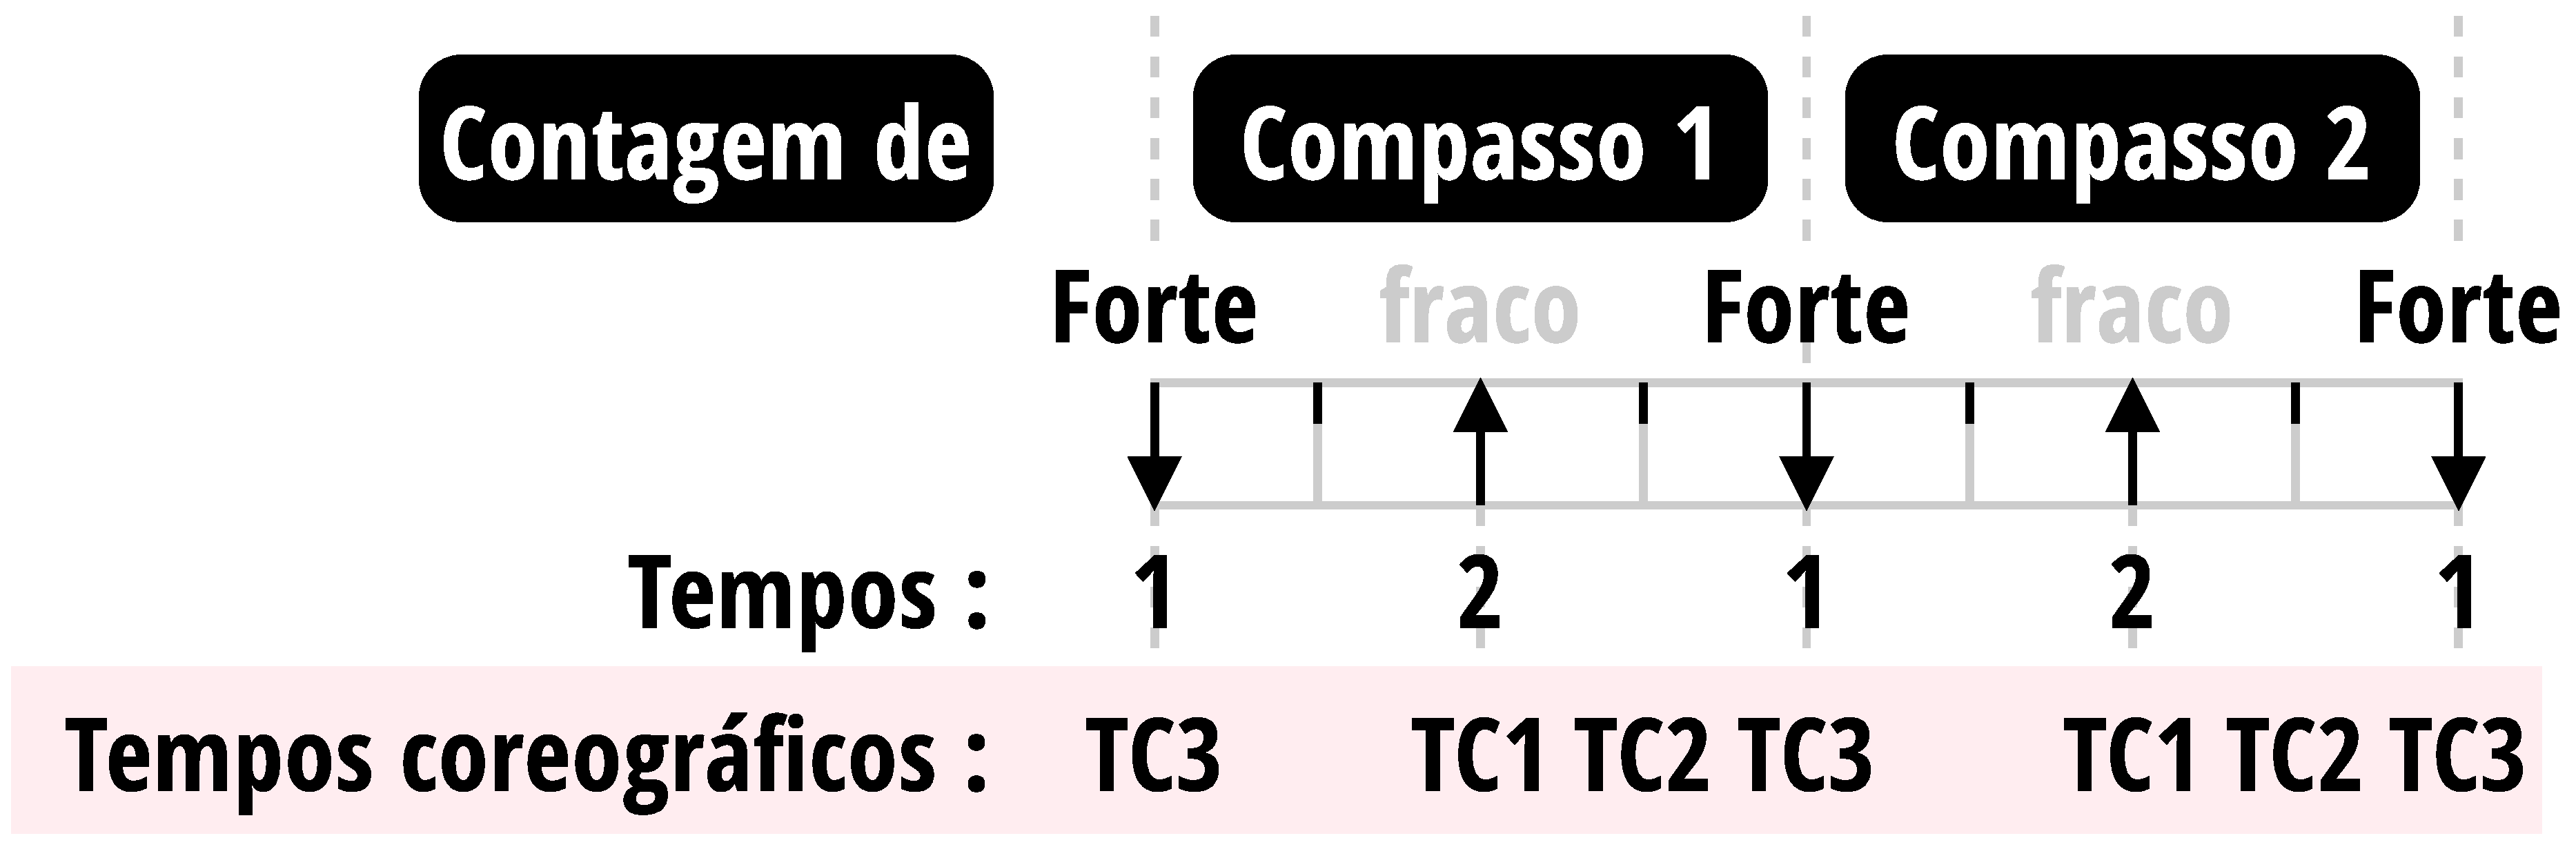
\includegraphics[width=\textwidth]{chapters/cap-musicalidade/contagemtempocoreografico.eps}
\begin{abc}[name=abc-contagemtempocoreografico]
X: 1 % start of header
K: C stafflines=1 % scale: C major
M: 2/4 %meter - compasso
%Q:1/4=80
V:1 clef=perc stem=up %name="Pauta com clave de fá"   sname="Pauta com clave de fá"
[V:1] |: B2 B1 B1| B2 B1 B1 | B2 B1 B1 :|
w: ~ TC1 TC2 TC3 TC5 TC6 TC7 
w: ~ 2_ 1  2_ 1 ~  
\end{abc}
    \vspace{-20pt}
    \caption{Contando tempos coregráficos.}
    \label{fig:contagemtempocoreografico}
\end{figure}



%%%%%%%%%%%%%%%%%%%%%%%%%%%%%%%%%%%%%%%%%%%%%%%%%%%%%%%%%%%%%%%%%%%%%%%%%%%%%%%%
%%%%%%%%%%%%%%%%%%%%%%%%%%%%%%%%%%%%%%%%%%%%%%%%%%%%%%%%%%%%%%%%%%%%%%%%%%%%%%%%
\section{Procurando um bom ``Timing''}
\index{Musicalidade!Timing}

\begin{definition}[Timing:]
é uma palavra em inglês, que é usada no vocabulario da dança, 
para indicar o grau de exatitude temporal\footnote{%
Sincronização,
sentido de oportunidade \cite{TimingDef}.} 
na execusão de uma sequencia de movimentos.% no momento previsto.
\end{definition}

O Prof. Victor Hugo Suárez dedicado ao ensino de bailes esportivos e danças latinas,
indica que quando falamos que temos um bom timing \cite{TimingDef2} em nossos movimentos de pés, 
nos referimos à capacidade de colocar o peso total do corpo ao principio de cada tempo planejado;
deste jeito estaremos com o peso bem definido e teremos mais tempo 
(o tempo completo entre movimentos  consecutivos), 
para executar corretamente as \hyperref[sec:musicalidade:dinamicas]{\textbf{dinâmicas}} 
planejadas para os movimentos.

Por outro lado os professores Jessie Ma e Clay Boonthanakit
indicam \cite{TimingDef3} que para conseguir uma performance limpa na sua dança,
ter um bom timing, e
um dos fatores\footnote{São indicados 3 fatores para ter uma performance limpa na dança,
estes são: ter um correta posição ou postura em cada movimento, ter um bom timing, e 
acertar o sentimento da música.} importantes a seguir.

\begin{example}
\label{ex:timing1}
Uma pessoa deve executar em bucle, ou reproduzir usando algum software informático,
alguma das sequencias rítmicas descritas na Figura \ref{fig:ex:timing}.
A pessoa que deseja treinar seu timing deve tentar caminhar, ou em geral, 
mexer os pés para acompanhar o ritmo escutado,
ate o ponto de que deve parecer que são os pés da pessoa que executam o ritmo.

Outras indicações para o exercício seriam:
\begin{itemize}
\item Deve-se procurar que o peso do corpo esteja bem definido num pé só 
ao inicio de cada som no ritmo escolhido.
\item Para agregar maior complexidade podem dar palmas em cada tempo forte.
\end{itemize}
\end{example}


\begin{figure}[ht]
\centering
\begin{subfigure}{.45\textwidth}
  \centering
  % include first image
  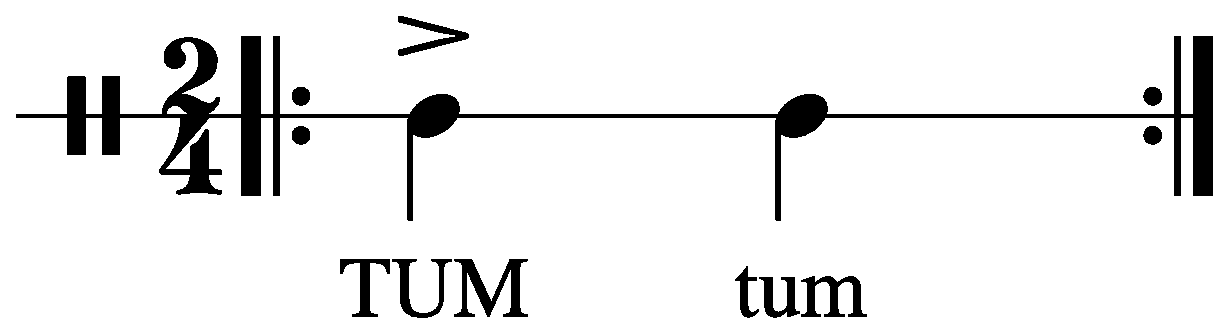
\includegraphics[width=.8\linewidth]{chapters/cap-musicalidade/timing0-1.eps}  
  \caption{Ritmo de treinamento 1.}
  \label{fig:ex:timing:a}
\end{subfigure}
\hfill	
\begin{subfigure}{.45\textwidth}
  \centering
  % include second image
  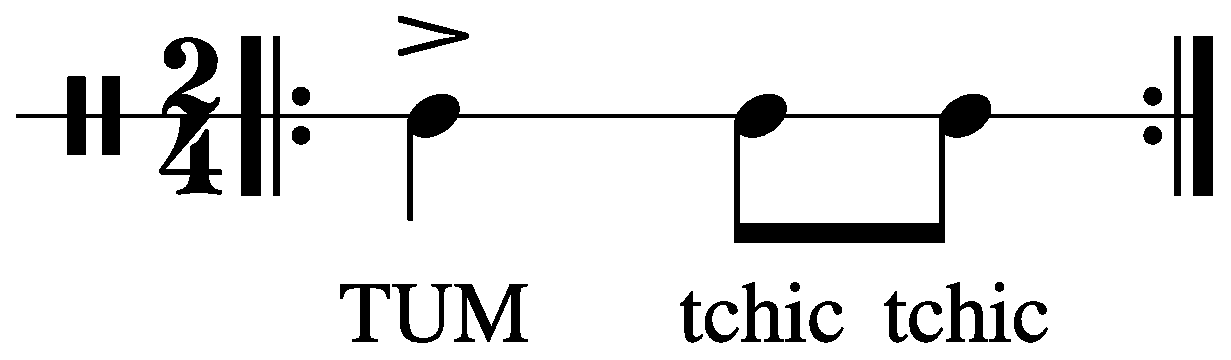
\includegraphics[width=.8\linewidth]{chapters/cap-musicalidade/timing1-1.eps}  
  \caption{Ritmo de treinamento 2.}
  \label{fig:ex:timing:b}
\end{subfigure}
\hfill
\begin{subfigure}{.65\textwidth}
  \centering
  % include second image
  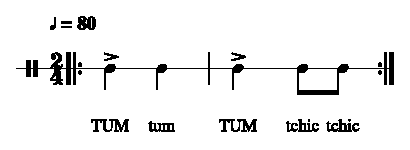
\includegraphics[width=.8\linewidth]{chapters/cap-musicalidade/timing2-1.eps}  
  \caption{Ritmo de treinamento 3.}
  \label{fig:ex:timing:c}
\end{subfigure}
\caption{Possíveis ritmos usados para o treinamento.}
\label{fig:ex:timing}
\end{figure}

O professor de dança Cleidson Diniz propõe \cite{TimingTreino1} 
o exercício descrito no Exemplo \ref{ex:timing:diniz},
\begin{example}
\label{ex:timing:diniz}
Uma pessoa deve jogar ao ar um objeto leve\footnote{A ideia de usar um objeto leve 
é que este não faça barulho ao cair no chão.}, 
e outra pessoa deve bater palmas\footnote{Pode ser trocado por uma pisada forte.}, 
uma vez, no momento exato que este chegue ao chão.
Este exercício pode ser variado tendo em conta o seguinte.
\begin{itemize}
\item A pessoa que vai bater as palmas vê em todo momento a trajetória do objeto.
\item A pessoa que vai bater as palmas só vê o inicio da trajetória. 
Pois o objeto é jogado na sua frente para suas costas.
\item A pessoa que vai bater palmas está com os olhos fechados
e segurando o braço da pessoa que joga o objeto,
de modo que a única informação que tem, 
para predizer o momento do contato do objeto com o chão, 
é o movimento do braço. 
\end{itemize}
\end{example}

%%%%%%%%%%%%%%%%%%%%%%%%%%%%%%%%%%%%%%%%%%%%%%%%%%%%%%%%%%%%%%%%%%%%%%%%%%%%%%%%
%%%%%%%%%%%%%%%%%%%%%%%%%%%%%%%%%%%%%%%%%%%%%%%%%%%%%%%%%%%%%%%%%%%%%%%%%%%%%%%%
% variar el timing implica trabalhar com dinamicas





\section{Usando as frases musicais}
Quando dançamos realizamos movimentos, 
concatenando eles um apos de outro para formar estruturas mais complexas;
porém, nós não dançamos sem executar pausas ou colocando aleatoriamente a velocidade 
e expressividade dos movimentos; 
se não que procuramos que estes tenham sentido, 
e inclusive trabalhamos para que os movimentos mostrem algum tipo de ordem, mensagem emocional ou simbólico.
Com este propósito, na dança, podemos agrupar nossos movimentos em frases ``coreográficas'';
é dizer, um grupo de movimentos, que expressa por sim mesmo uma ideia completa, 
e que tem algum indicador de final. 

Assim, na dança, 
nós criaremos estruturas maiores usando estas frases coreográficas, 
que guardam em sim mesma um sentido; 
neste ponto percebemos que devemos escolher a ideia a transmitir;
a escolha desta informação é pessoal, porém uma fonte de informação comumente escolhida é a música.
Aqui é usado o termo ``comumente'', porque mesmo se tiramos a música, 
e observamos a um par de dançarinos experimentados realizando uma coreografia, 
poderemos observar um sentido e estética no seus movimentos,
além de uma introdução, ideias completas, um \hyperref[ref:climax]{\textbf{clímax}}  e um final.
Em alguns casos os dançarinos usam a música só como um marco emocional,
para transmitir a informação de uma historia que nasce na cabeça dos dançarinos;
mas é claro que quantos mais aspectos da música sejam interpretados na dança,
o produto final terá um aspecto de maior musicalidade.

Na procura da musicalidade, uma boa escolha é conseguir que nossas frases coreográficas,
coincidam comas frases musicais;
para conseguir isto nós devemos aprender a 
\hyperref[sec:perceberfrases]{\textbf{identificar as frases musicais}}\footnote{O 
tema da percepção de frases musicais foi tratado na Seção \ref{sec:perceberfrases}},
de modo que  nossa frase coreográfica acompanhe à frase musical.

A continuação presentamos uma serie de exemplos de exercícios, 
que nós ajudarão a desenvolver a capacidade de dançar seguindo as frases musicais,
ate tornar esta atividade mais cotidiana.

\begin{example}[Dançando em frases de 4 compassos:]
\label{ex:usandofrases1}
(2 movimentos)
Primeiro escolheremos uma música com frases de 4 compassos, como ``Piston de gafieira'' de Billy Blanco,
ou algumas das mostradas no Exemplo \ref{ex:frasesde4compassos}.
Logo procederemos a executar em cada frase musical uma frase coreográfica, de um total de duas;
de modo que a primeira frase coreográfica leva o nome ``movimento 1'' e a segunda ``movimento 2''.

Com a distribuição de tempos dos movimentos, da Figura \ref{fig:frasecoreografica0}, 
podemos escolher distintos tipos de movimentos para as frases coreográficas, 
como\footnote{Sim 
se quer agregar um pouco mais de complexidade ao exercício,
pode-se dar palmas no primeiro tempo de cada frase musical.}:
\begin{itemize}
\item \textbf{movimento 1:} caminhar para adiante.
\item \textbf{movimento 2:} caminhar para atrás.
\end{itemize}
Outra  escolha alternativa de movimentos pode ser:
\begin{itemize}
\item \textbf{movimento 1:} realizar um balanço.
\item \textbf{movimento 2:} caminhar para adiante ou atrás. 
Se o exercício se realiza em pares o abraço de dança pode ser aberto, 
com uma caminha ao lado (de malandro). 
\end{itemize}
\end{example}


\begin{figure}[!h]
    \centering
    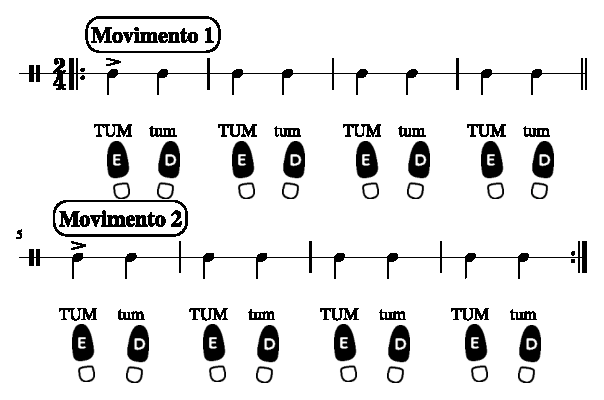
\includegraphics[width=0.99\textwidth]{chapters/cap-musicalidade/treino-fraseio0-1.eps}
    \caption{Duas frases coreográficas de 4 compassos.}
    \label{fig:frasecoreografica0}
\end{figure}

\begin{example}[Dançando em frases de 4 compassos:](2 movimentos)
De forma similar ao Exemplo \ref{ex:usandofrases1},
usaremos uma frase de 8 tempos, 
e usando uma distribuição de tempos dos movimentos, como na Figura \ref{fig:frasecoreografica1a}, 
podemos escolher distintos tipos de movimentos para as duas  frases coreográficas, 
como\footnote{Sim 
se quer agregar um pouco mais de complexidade ao exercício,
pode-se dar palmas no primeiro tempo de cada frase musical.}:
\begin{itemize}
\item \textbf{movimento 1:} realizar um balanço.
\item \textbf{movimento 2:} realizar o cruzado.
\end{itemize}
Outra  escolha alternativa de movimentos pode ser:
\begin{itemize}
\item \textbf{movimento 1:} realizar um balanço.
\item \textbf{movimento 2:} realizar o frente trás (básico linear).
\end{itemize}
Em ambos casos devemos seguir a distribuição de tempos indicada no último compasso de cada frase 
para ir ao movimento seguinte.
\end{example}

\begin{figure}[!h]
    \centering
    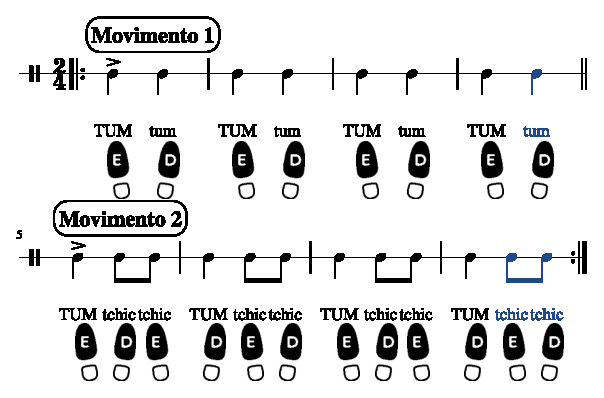
\includegraphics[width=0.99\textwidth]{chapters/cap-musicalidade/treino-fraseio1a-1.eps}
    \caption{Duas frases coreográficas de 4 compassos.}
    \label{fig:frasecoreografica1a}
\end{figure}


\begin{example}[Dançando em frases de 4 compassos:](3 movimentos)
Primeiro escolheremos uma música com frases de 4 compassos, 
como ``Disritmia'' interpretado por Martinho da Vila,
ou algumas das mostradas no Exemplo \ref{ex:frasesde4compassos}.
Logo procederemos a executar em cada frase musical uma frase coreográfica.
A primeira frase coreográfica leva o nome ``movimento 1'', 
a segunda ``movimento 2''  e a terceira ``movimento 3''.


Com a distribuição de tempos dos movimentos, da Figura \ref{fig:frasecoreografica2a}, 
podemos escolher distintos tipos de movimentos para as frases coreográficas, 
como\footnote{Sim 
se quer agregar um pouco mais de complexidade ao exercício,
pode-se dar palmas no primeiro tempo de cada frase musical.}:
\begin{itemize}
\item \textbf{movimento 1:} realizar um balanço.
\item \textbf{movimento 2:} realizar o cruzado.
\item \textbf{movimento 3:} realizar o frente trás (básico linear).
\end{itemize}
Em todos casos devemos seguir a distribuição de tempos indicada no ultimo compasso de cada frase para ir ao movimento seguinte.

\end{example}

\begin{figure}[!h]
    \centering
    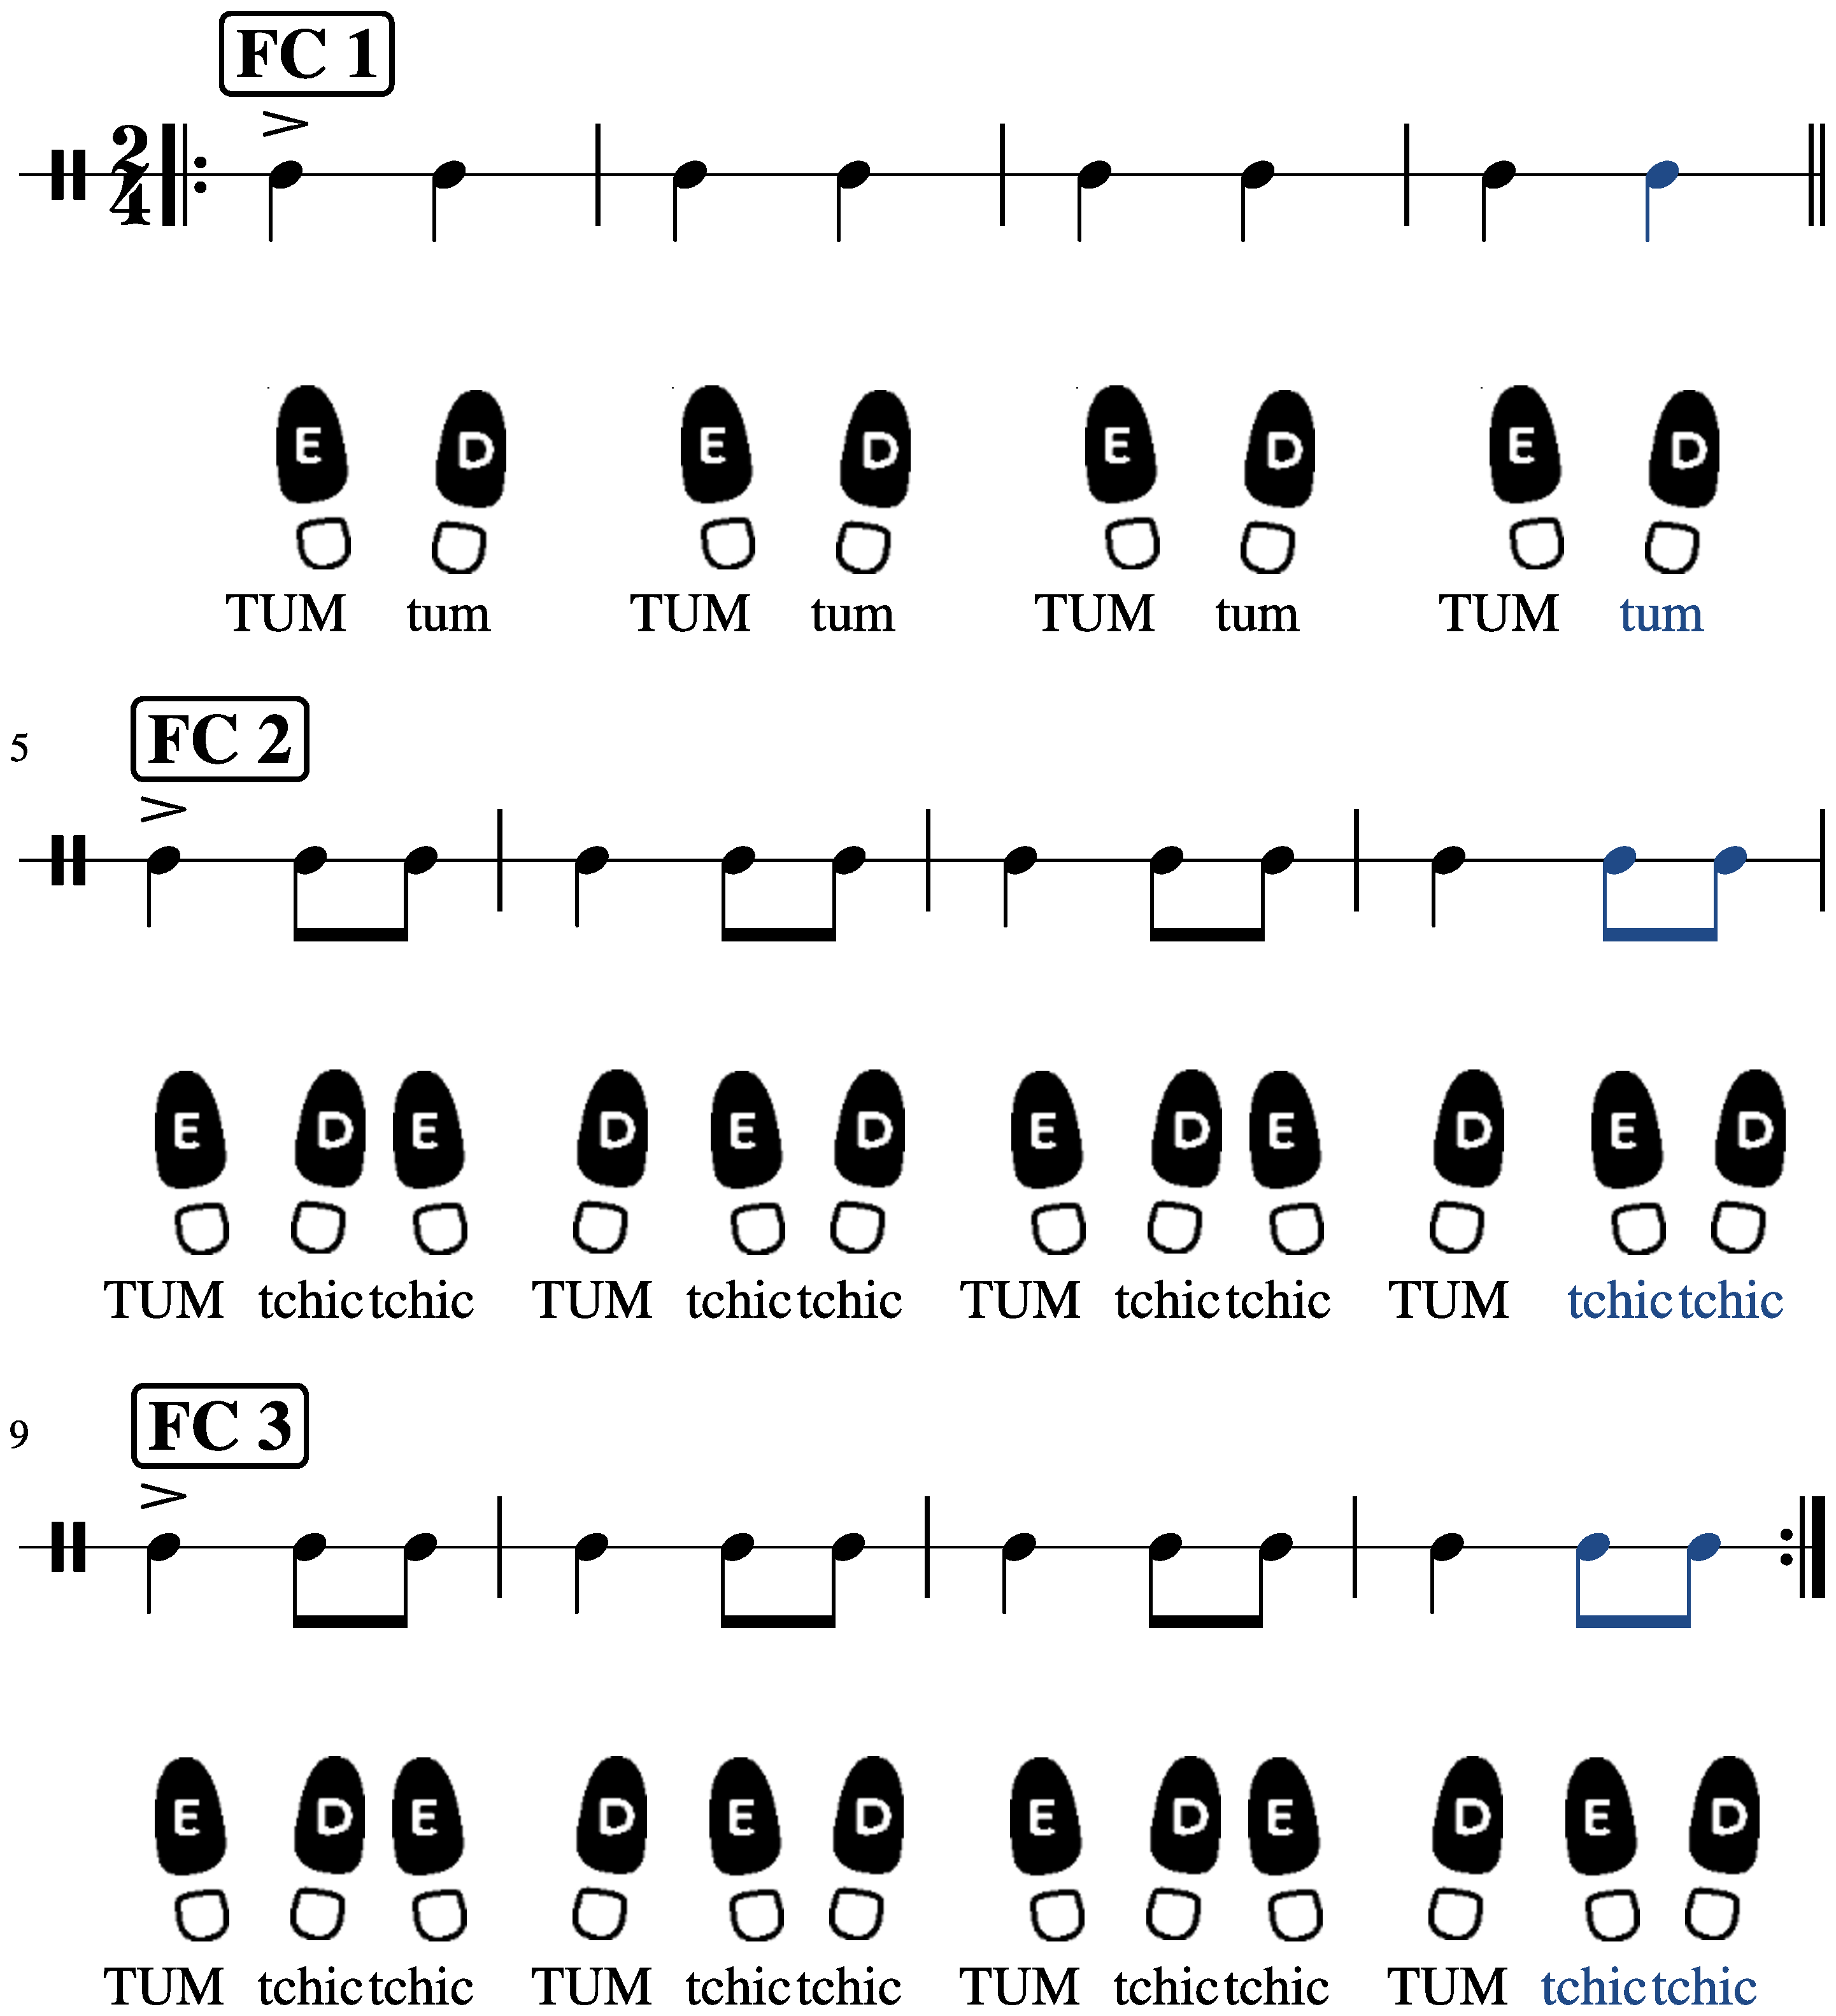
\includegraphics[width=0.9\textwidth]{chapters/cap-musicalidade/treino-fraseio2a-1.eps}
    \caption{Duas frases coreográficas de 4 compassos.}
    \label{fig:frasecoreografica2a}
\end{figure}

\begin{comment}
\subsection{Interpretando o tipo de final da frase}
\begin{itemize}
\item Si tentamos dançar no tempo forte, conhecer a existência de ambos tipos de final de frase, 
no ajuda a ter certeza que estamos indo bem com o tempo, e que não somos nos que erramos achando o tempo forte,
e sim, que existe mais de um tipo de final de frase, e que este foi diferente, foi suspensivo.
E não nos deixaremos enganar por finais suspensivos sincopados (que parecem conclusivos),
e estaremos mais seguros de nossa dança.
\item Uma vez temos ciência da existência de ambos tipos de final, 
podemos usar suas particularidades. Por exemplo,
uma frase com final conclusivo indica o fim, literal, de uma ideia musical, 
pelo que si desejamos ter coerência com a música, 
nosso movimento e parada deve demostrar a mesma resolução,
e dar a ideia de que o relato de nossa dança acabou de expressar uma ideia completa;
para isto podemos fazer um movimento explosivo com pausa abrupta, 
ou agregar uma postura final, ou tao simples como um abraço elegante com ponto final.
Por outro lado, se o final de frase musical é suspensivo, 
a ideia transmitida tem uma sensação de pergunta,
ou de uma resposta meditativa que se apaga aos poucos e pede uma reflexão ao ouvinte,
em outras palavras um assunto não completamente  concluído.
Nesse sentido, se nosso objetivo é ter uma coerência com a música,
o relato que expressa nossa dança deve dar essa sensação de uma ideia que se apaga aos poucos,
ou de pergunta; por exemplo, isto se consegue dando um passo final em tempo forte,
seguido de movimentos corporais no lugar ate a ultima nota musical.
\end{itemize}
\end{comment}





%%%%%%%%%%%%%%%%%%%%%%%%%%%%%%%%%%%%%%%%%%%%%%%%%%%%%%%%%%%%%%%%%%%%%%%%%%%%%%%%
%%%%%%%%%%%%%%%%%%%%%%%%%%%%%%%%%%%%%%%%%%%%%%%%%%%%%%%%%%%%%%%%%%%%%%%%%%%%%%%%

%%%%%%%%%%%%%%%%%%%%%%%%%%%%%%%%%%%%%%%%%%%%%%%%%%%%%%%%%%%%%%%%%%%%%%%%%%%%%%%%
%%%%%%%%%%%%%%%%%%%%%%%%%%%%%%%%%%%%%%%%%%%%%%%%%%%%%%%%%%%%%%%%%%%%%%%%%%%%%%%%
\clearpage
\section{Usando o ``break'' da música}
\label{sec:UsandoBreak}
\index{Musicalidade!Breques}
\index{Musicalidade!Break}

Na Seção \ref{sec:percepcionbreak} foram apresentadas um conjunto de dicas 
para poder detetar os breques (breaks) na música.
Com esta informação um dançarino pode incorporar este aspecto da música na sua dança;
assim, nesta seção apresentaremos um conjunto de sugestões  
de como podemos interpretar os breques\footnote{Estas 
sugestões entram na categoria de ``mapeamento'' de aspectos da música, 
explicado na Figura \ref{fig:interpretacion-corporal}.}.

Entre a lista de sugestões de mapeamento, 
entre o break e os aspectos do movimento, 
temos que:
\begin{itemize}
\item Quando acontece uma pausa (breque) total na música, 
é interessante acompanhar este aspecto realizando também uma pausa total em nossos movimentos.
\item Se o breque acontece,
e um solo melódico ou percussivo preenche a pausa;
então nós temos duas opções, 
\begin{itemize}
\item ou desprezar o solo e permanecer inativos\footnote{Se por exemplo o solo é curto demais.},
\item ou utilizar o solo musical e realizar um solo de dança\footnote{Mesmo se o solo é curto.};
é dizer, realizar uma dança que incorpore aspectos do solo musical,
de modo que fique evidente que é um intermédio entre duas propostas de movimentos,
a anterior e a posterior ao breque.
\end{itemize}
\item Se decidimos dançar o solo no break, 
então podemos lembrar que 
\begin{itemize}
\item é comum mapear movimentos de pés ou de deslocamento ao ritmo 
(acompanhamento ou ritmo da melodia), e 
\item movimentos corporais quase sem deslocamento a aspectos da melodia (mudança de tons, tensão, articulação, etc.).
\end{itemize}
Também existe a possibilidade de misturar ambas técnicas usando movimentos corporais e deslocamento,
se o solo no breque é o suficientemente longo.
\item Também poderíamos simplesmente dançar o silencio da pausa, colocando um movimento corporal sem deslocamento,
para não perder a inercia, até iniciar a seguinte frase musical.
\item Quando decidimos dançar a pausa no break e temos um par de dança,
podemos estar separados ou usar um abraço de dança (fechado ou aberto).
\begin{itemize}
\item Se o abraço é fechado, os movimentos do condutor estarão mais limitados,
e este deverá conduzir os movimentos ao seguidor.
\item Se o par de dança está separado ou o abraço é aberto, 
o seguidor e condutor tem mais liberdade de movimento,
e se desejam podem executar cada um seus movimentos independentemente,
sem necessidade de condução. 
\end{itemize}
Entre os movimentos que poderíamos usar no break, estão por exemplo, 
um samba no pé, um bamboleio circular de quadril (no plano axial), um balanço de ombros (no plano frontal), etc. 
\item Uma vez finalizado o solo, é mais fácil iniciar a seguinte frase musical
no seu primeiro \hyperref[subsec:perceberTF1]{\textbf{tempo forte}}. 
Assim, 
ao finalizar o solo devemos ter bem definido o peso do corpo num pé,
para ter rapidez a iniciar a seguinte frase.
\item Também é interessante esperar o inicio da frase apos o break, 
com os pés próximos; pois se etão separados, 
dar um passo em tempo forte para iniciar a frase musical será difícil,
pois os pés já estariam separados.
\end{itemize}~

No Exemplo \ref{ex:breakvarios} indicamos um conjunto de músicas 
que são ótimas para o treinamento de forma unipessoal,
pois tem uma grande quantidade de breques, 
e solos nos breques.
\begin{example}[Músicas com muitos breques]~
\label{ex:breakvarios}
Em todos os exemplos listados, os breques acontecem na linha melódica principal e o acompanhamento,
enquanto que o cantor faz solos falando; 
dado que a voz é quase de um tom uniforme e não poderia ser considerada preponderantemente melódica,
se sugere, sim se deseja dançar o solo, que se aproveite só ritmicamente a voz.
\begin{itemize}
\item ``Idade não é documento'' interpretado por Moreira da silva.
\item ``Jogando com o capeta'' interpretado por Moreira da silva.
\item ``Na subida do morro'' interpretado por Moreira da silva. 
O primeiro break é feminino.
\end{itemize}
\end{example}

Outras músicas com breaks podem ser encontradas nos Exemplos \ref{ex:breakmasculinos},
\ref{ex:breakfeminino} e 
\ref{ex:breaksincopados}.

\newpage
%%%%%%%%%%%%%%%%%%%%%%%%%%%%%%%%%%%%%%%%%%%%%%%%%%%%%%%%%%%%%%%%%%%%%%%%%%%%%%%%
%%%%%%%%%%%%%%%%%%%%%%%%%%%%%%%%%%%%%%%%%%%%%%%%%%%%%%%%%%%%%%%%%%%%%%%%%%%%%%%%
\section{Usando dinâmicas na dança }
\label{sec:musicalidade:dinamicas}
\index{Musicalidade!Texturas}
\index{Musicalidade!Dinâmicas}

O termo ``textura'' é uma metáfora usada na dança para referenciar 
o como percebemos que um movimento é feito \cite[pp. 127,268,270]{preston1995dance}.
Por exemplo, quando pensamos na textura de um material,
imaginamos que este pode ser liso, áspero, macio, sedoso, sólido, pontiagudo, fluido, seco, úmido, etc. 
Da mesma forma, quando usamos a metáfora  da textura na dança,
nos referimos às múltiplas formas que podemos observar na execução de um movimento (material).

Além da metáfora da textura, podemos usar mais formalmente o termo ``dinâmica'', 
para referenciar à forma (expresividade) em que um movimento é feito;
por exemplo este pode ser: suave, forte, pesado, elástico, acentuado, nítido com varições de tempo e tensão \cite[pp. 268]{preston1995dance}
\cite[pp. 10]{cullingford2013children} \cite[pp. 424, 447]{guest2013labanotation};
ou de forma geral podemos indicar o uso da energia, do peso do corpo, da resistência, e do tono muscular e emocional \cite[pp. 424]{cullingford2013children}.
Só poderia agregar pequenas diferencias no uso destes termos;
quando usamos o termo ``dinâmica'' nos referimos geralmente à criação de um movimento, 
utilizando determinado procedimento;
enquanto que o termo textura, seguindo a metáfora da observabilidade, 
se refere à forma como percebemos que um movimento foi criado, utilizando  um determinado procedimento.
Na prática ambos termos são usados pra descrever a mesma coisa: A forma como é feito um movimento;
por exemplo, podemos ter frases como: ``os movimentos dos dançarinos tem texturas diferentes! Que dinâmicas usaram?''
ou ``os dançarinos realizam dinâmicas diferentes! Qual textura você gostou?''.

\begin{tcbattention}
Devemos lembrar que o termo \hyperref[sec:texturasmusica]{\textbf{textura}} 
é usado também na música, 
para descrever o modo em que interagem e se misturam várias linhas melódicas,
este tema já foi abordado na Seção \ref{sec:texturasmusica}.
Assim para evitar confusões é mais eficiente usar o termo dinâmica,
ou especificar o âmbito com frases como ``a textura do movimento''.
\end{tcbattention}


\begin{tcbinformation} 
\label{ref:importanciadinamicas}
\textbf{Por que as dinâmicas são importantes na dança?}
O uso de diferentes dinâmicas permite criar muitas variações de um mesmo movimento.
Por outro lado, como cada dinâmica tem uma aparência diferente,
esta pode ser associada a um som especifico na música.
Por exemplo, a um sonido grave como de um bumbo,
lhe poderia corresponder um andar pesado, como de um elefante.
\end{tcbinformation} 

\begin{example}
\label{ex:word:bank}
\textbf{Termos usados para definir dinâmicas:} 
A seguir são listados alguns termos que poderíamos usar 
para indicar a textura que poderia adotar uma determinada dinâmica \cite[pp. 31]{paine2014complete}:

\begin{tasks}(4)
\task tenso
\task fluido
\task enérgico
\task lento
\task pesado
\task explosivo
\task poderoso
\task suave
\task delicado
\task robótico
\task elástico
\task gentil
\task relaxado
\task espasmódico
\task rápido
\task mole
\end{tasks}
\end{example}


\begin{example}[Listando dinâmicas:]
\label{ex:dinamicas:treino1}
Pense num movimento corporal, por exemplo dar um passo adiante,
logo liste todas as formas que podem ser adotadas para dar esse passo (Por 
exemplo as palavras listadas no Exemplo \ref{ex:word:bank}). 
\end{example}

\begin{example}[Usando dinâmicas:]
\label{ex:dinamicas:treino2}
Usando a lista de dinâmicas, elaborada no Exemplo \ref{ex:dinamicas:treino1},
execute um mesmo movimento corporal usando  todas essas dinâmicas.
\end{example}


%%%%%%%%%%%%%%%%%%%%%%%%%%%%%%%%%%%%%%%%%%%%%%%%%%%%%%%%%%%%%%%%%%%%%%%%%%%%%%%%
\subsection{Fatores do movimento: Modelo de Laban (esforço)}
\label{subsec:fatordinamica}

\begin{tcbinformation} 
\label{ref:eukinetic}
\index{Musicalidade!Eucinética}
\index{Musicalidade!Eukinética}
\textbf{Eucinética (Eukinética):}
Termo criado por Rudolf Laban usando as palavras gregas ``Eu'', que significa bom,
e ``Kinesis'' que significa movimento.
A eucinética é o estudo dos aspectos qualitativos do movimento,
que compreende os quatro fatores do movimento: Fluência,  espaço,  peso  e  tempo 
\cite[pp. 25-26]{elementosdanca2017} \cite[pp. 97]{maletic2011body}.
%Pode-se especular que ele cunhou o termo para diferenciar seu trabalho de vários métodos eurítmicos \cite[pp. 97]{maletic2011body}.
\end{tcbinformation} 


O  analises do movimento feito por Rudolf Laban, 
descrito no seu livro ``Domínio do Movimento'' \cite[pp. 28]{laban1987dominio},
indica que podemos separar as dinâmicas que realizamos com nossos movimentos
(ou esforço na notação de Laban), 
em quatro diferentes fatores ou categorias (ver Figura \ref{fig:fatores:moviemnto:Laban})
\cite[pp. 142]{laban1987dominio} 
\cite[pp. 93]{maletic2011body}
\cite[pp. 30]{paine2014complete}
\cite[pp. 5]{carline2011lesson}: 
\begin{tasks}(4)
\task Peso
\task tempo 
\task espaço 
\task fluência
\end{tasks}

\begin{wrapfigure}{r}{0.5\textwidth}
\centering
\smartdiagramset{
  text width=5.5cm,
  module minimum width=3.5cm,
  module minimum height=1.5cm
} 
\smartdiagram[bubble diagram]{Fatores do\\movimento,Peso,Tempo,Espaço,Fluência}
\caption{Fatores do movimento no modelo de Rudolf Laban.}
\label{fig:fatores:moviemnto:Laban}
\end{wrapfigure}
A seguir vemos uma descrição detalhada de todos estes fatores:\\
\begin{description}
\item[Peso:]
Refere-se o grau de tensão corporal necessário para a execução de uma ação, 
onde pode-se estar em algum ponto intermediário entre o firme e o leve 
(em inglês é conhecido como   ``firm'' e ``fine'') 
\cite[pp. 137, 143]{laban1987dominio}  \cite[pp. 5]{carline2011lesson} \cite[pp. 28]{elementosdanca2017}. 
\begin{itemize}
\item Firme: Os músculos estão tensionados, são uma fonte de resistência ao peso. Exemplos: O andar de um elefante, socos ou explodir.
\item Leve: Temos uma leve tensão muscular e um toque suave ou delicado,
tem uma leve resistência ao peso.  Exemplos: Ligeiro, flutuar.
\end{itemize}~
%%
\end{description}

\begin{description}
\item[Tempo:] Refere-se ao modo do uso do tempo no movimento,
onde pode-se estar em algum ponto intermediário entre o súbito e o sustentado 
(em inglês é conhecido como    ``sudden'' e ``sustained'') 
\cite[pp. 143]{laban1987dominio} \cite[pp. 5]{carline2011lesson} \cite[pp. 28]{elementosdanca2017}.
\begin{itemize}
\item Súbito: Envolve uma ação imediata e/ou surpreendente, é dizer de curta duração
ou com um sentir de momentaneidade. Exemplos: estancar-se numa posição, saltar.
\item Sustentado: O corpo leva um tempo para executar uma única ação, 
com um movimento persistente e contínuo, é dizer de duração indeterminada ou com um sentir interminável.  
Exemplos: Acomodar, afundar.
\end{itemize}~
\end{description}

\begin{description}
\item[Espaço:] Refere-se ao modo do deslocamento;
este pode estar em algum ponto intermediário entre  direto  e  flexível 
(em inglês é conhecido como  ``linear'' e ``curved'') 
\cite[pp. 143]{laban1987dominio} \cite[pp. 6]{carline2011lesson} \cite[pp. 28]{elementosdanca2017}.
\begin{itemize}
\item Linear: o movimento segue uma trajetória reta. Exemplo:
Um braço se estende de modo que a mão gere uma trajetória sobre uma linha,
com um sentir de estreiteza.
\item Curvado: O movimento tem movimentos realizando curvas ou torções,
com um sentir de movimentos manejáveis na sua extensão espacial. 
Exemplos: Um braço se estende de modo que a mão descreve uma meia lua e o antebraço realiza uma torção no seu eixo.
\end{itemize}~
%%
\item[Fluência :] (``flow'') Refere-se a quando nossos movimentos podem 
estar em algum ponto intermediário entre um movimento livre  e outro contido 
(em inglês é conhecido como   ``free'' e ``bound'')
\cite[pp. 140-143]{laban1987dominio} \cite[pp. 6]{carline2011lesson} \cite[pp. 27]{elementosdanca2017}.
\begin{itemize}
\item Livre: Quando o corpo se movimenta livremente num movimento continuo,
de modo que não existam emendas entre o final de um movimento e o inicio de outro.
\item Contido: Quando o movimento do corpo é interrompido,
de modo que é fácil distinguir como os movimentos estão estruturados em pedaços.
\end{itemize}~
\end{description}

%%%%%%%%%%%%%%%%%%%%%%%%%%%%%%%%%%%%%%%%%%%%%%%%%%%%%%%%%%%%%%%%%%%%%%%%%%%%%%%%
\subsection{Fatores de movimento: Um modelo atual}
\label{subsec:fator:movimento:atual}
\begin{wrapfigure}{r}{0.6\textwidth}
\centering
\smartdiagramset{
  text width=5.5cm,
  module minimum width=3.5cm,
  module minimum height=1.5cm
} 
\smartdiagram[bubble diagram]{Fatores do\\movimento,Força,Velocidade,Continuidade}
\caption{Fatores do movimento comumente usados.}
\label{fig:fatores:moviemnto:popular}
\end{wrapfigure}
Atualmente (\AnoLivro), muitos profissionais do mundo da dança, 
 acostumam usar modelos pedagógicos, 
com outras subdivisões diferentes aos fatores do movimento descritos por Laban; 
porém estes modelos também separam as dinâmicas dos movimentos em fatores;
por exemplo, é comum achar o modelo  mostrado na Figura \ref{fig:fatores:moviemnto:popular},
na literatura \cite[pp. 30]{paine2014complete} \cite[pp. 181]{smith2014dance}
e em meios audiovisuais que abordam temas relativos a dança:

\begin{description}
\item[Força:] (Suave $\rightarrow$ forte) 
É relativo à intensidade da força que usamos ao realizar nossos movimentos;
onde podemos escolher níveis de forças em algum ponto intermediário entre suave e forte. 
\end{description}

\begin{description}
\item[Velocidade:] (Lento $\rightarrow$ rápido)
Se refere à velocidade ao executar nossos movimentos;
onde podemos escolher velocidades em algum ponto intermediário entre lento e rápido. 
\item[Continuidade:] (Continuo $\rightarrow$ abrupto)
Refere-se ao grau de continuidade ao realizar nossos movimentos;
onde podemos escolher valores de continuidade em algum ponto intermediário entre continuo e abrupto.
\end{description}
Seja qual for a notação que usemos, sempre poderemos ordená-los em escalas
que tem dois extremos e infinitos pontos intermediários,
como é mostrado na Figura \ref{fig:element:moviment},
onde vemos como podemos realizar cada movimento selecionando umas caraterísticas especificas de força (F), velocidade (V) e continuidade (C);
é dizer com uma dinâmica (D),  $D=\{F, V, C\}$.
\begin{figure}[!h]
\centering
    \begin{subfigure}[b]{0.45\textwidth}
    \centering
    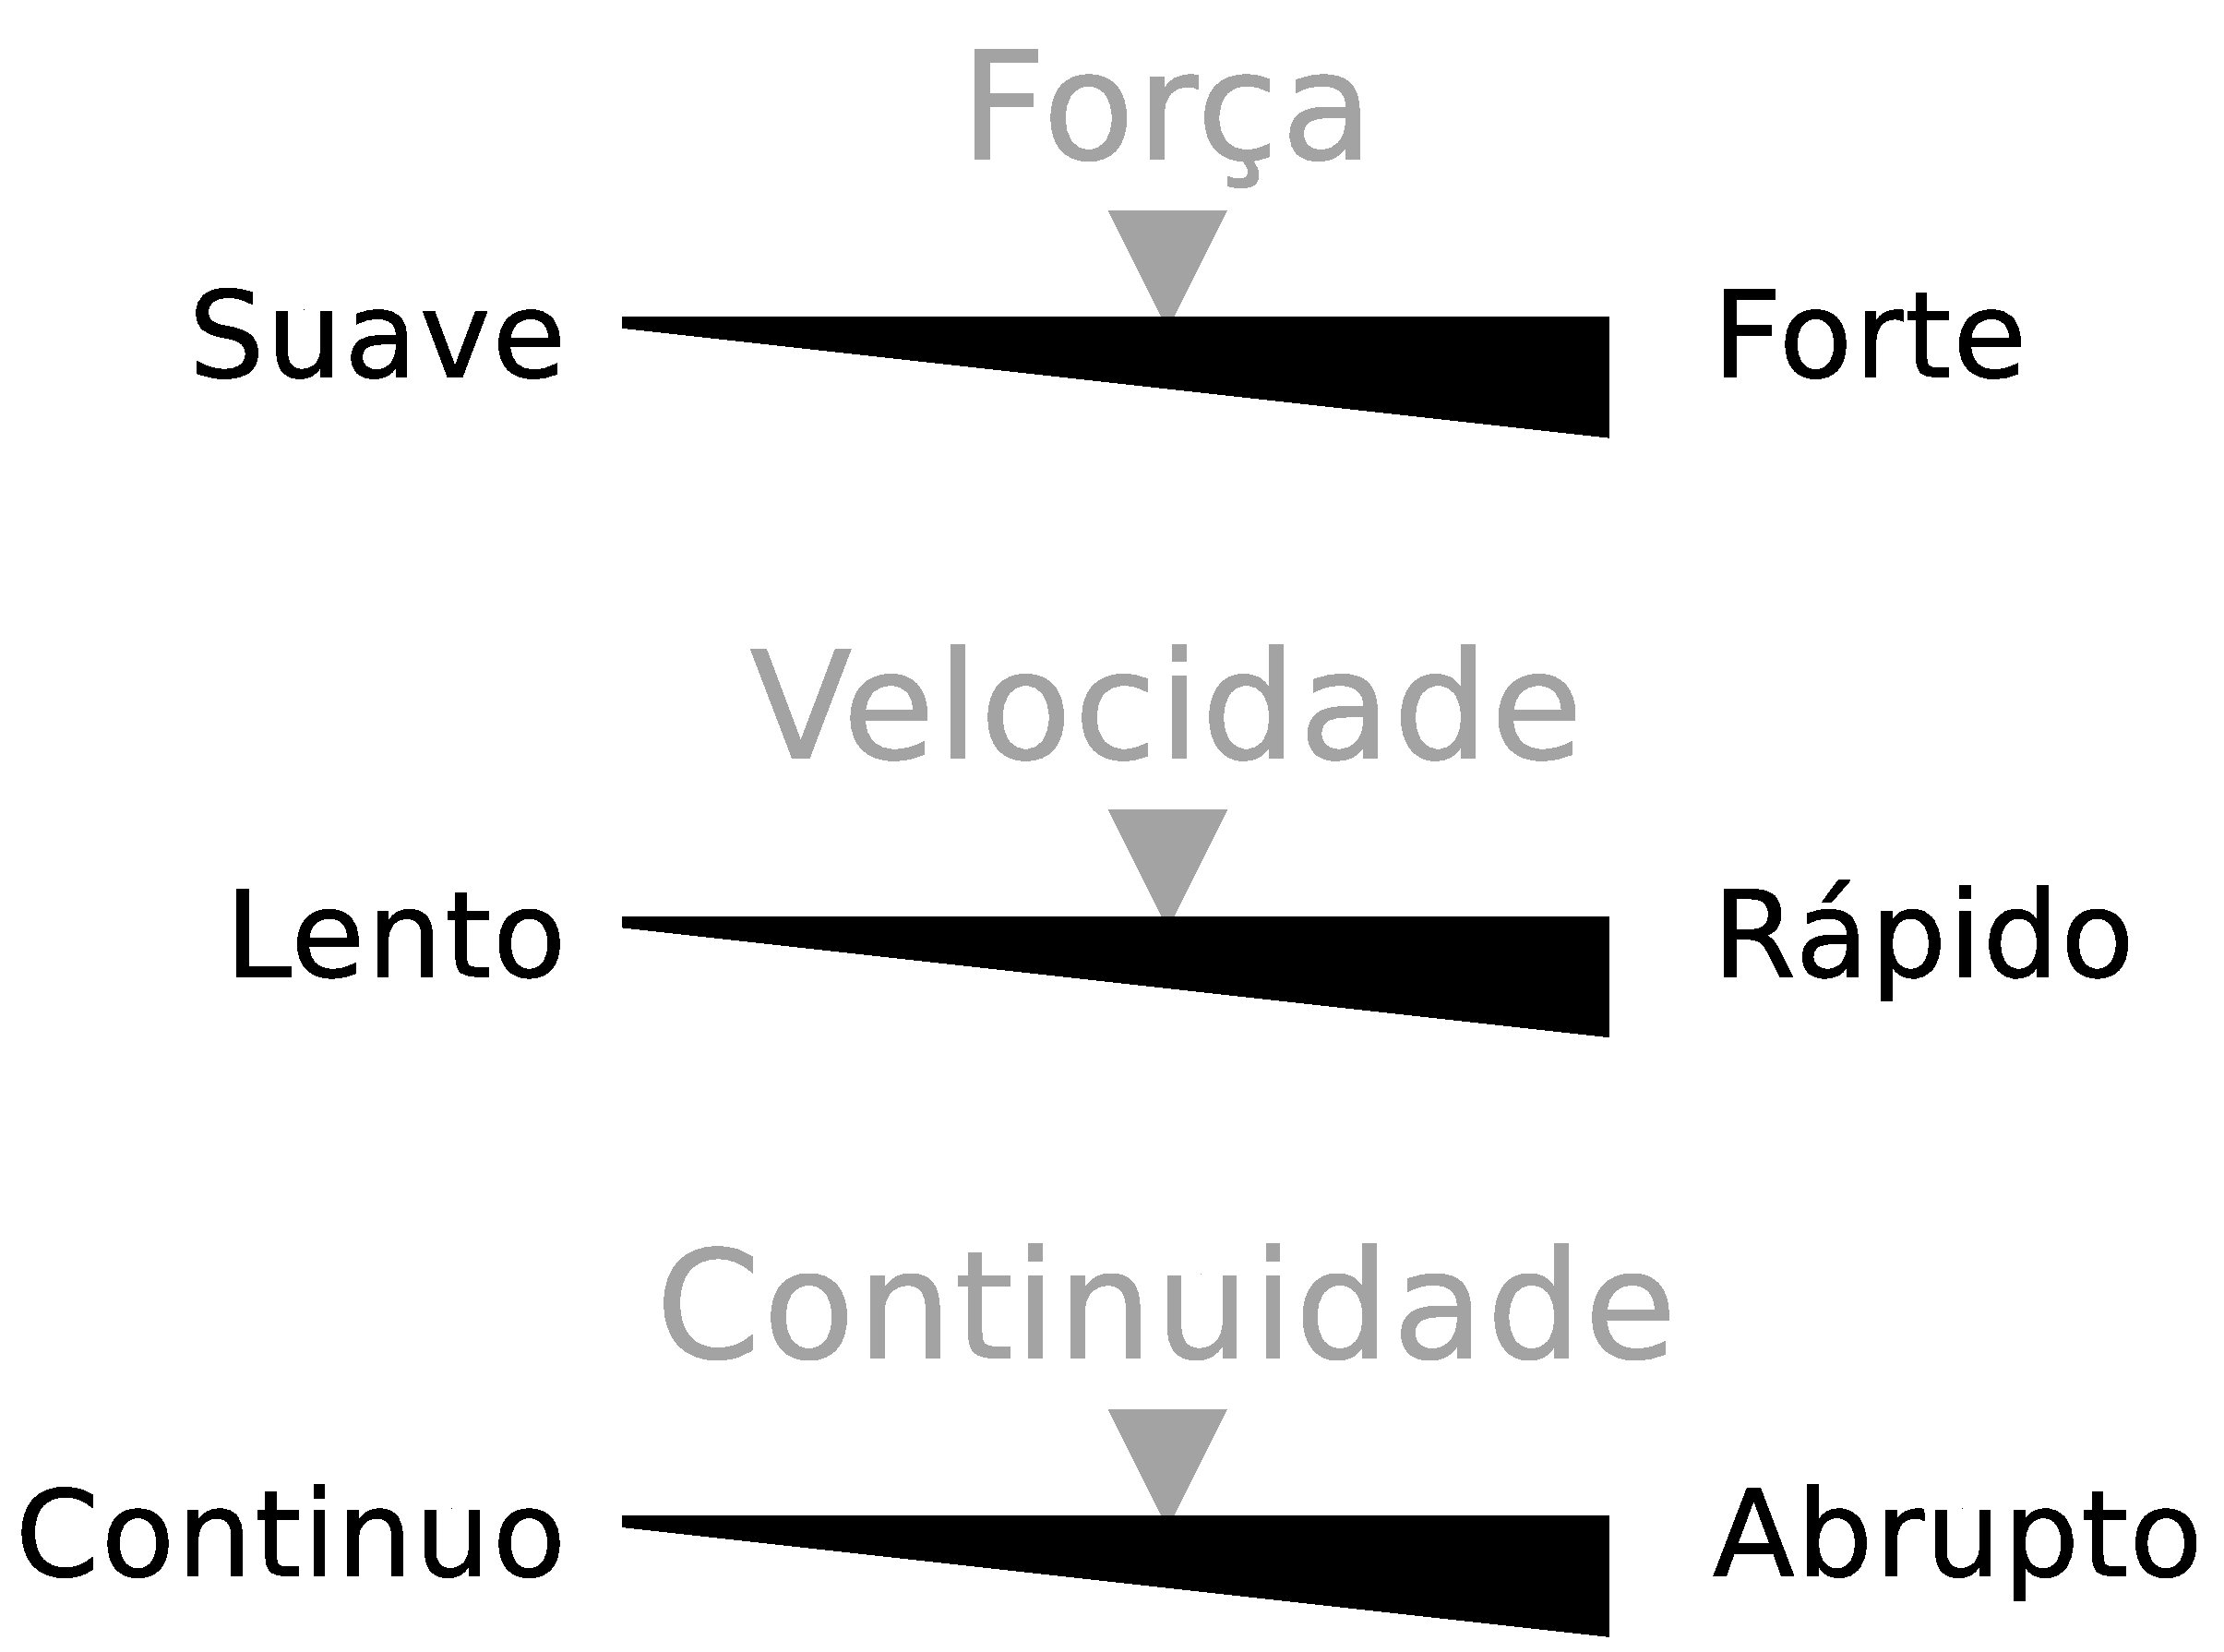
\includegraphics[width=0.95\textwidth]{chapters/cap-musicalidade/dinamicas-elementos1.eps}
    \caption{Caraterísticas do movimento.}
    \label{fig:element:moviment}
    \end{subfigure}
    \hfill
    \begin{subfigure}[b]{0.5\textwidth}
    \centering
    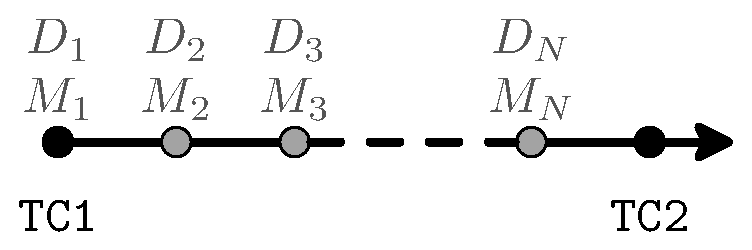
\includegraphics[width=0.95\textwidth]{chapters/cap-musicalidade/dinamicas-elementos1b.eps}
    \caption{Movimentos entre tempos coreográficos.}
    \label{fig:coreografia:moviment}
    \end{subfigure}
\caption{Dinâmicas dos movimentos.}
\label{fig:geral:moviment}
\end{figure}
Assim, podemos definir que entre dois \hyperref[sec:TemposCoreograficos]{\textbf{tempos coreográficos}} consecutivos,
podemos realizar coreografias com $N$ movimentos $M_n$, com $n=\{1, 2, ..., N\}$, 
de modo que a cada um destes movimentos lhe corresponda uma dinâmica $D_n=\{F_n, V_n, C_n\}$,
como pode ser visto na Figura \ref{fig:coreografia:moviment}.
\begin{example}[Explorando força e velocidade:]
Podemos estudar as dinâmicas de nossos movimentos fazendo um pequeno exercício,
primeiro escolheremos um movimento (M1), por exemplo: estirar os braços.
e depois usaremos 4 diferentes dinâmicas para executar-lho,
levando ao extremo as caraterísticas de força e velocidade,
e deixando num valor intermediário a continuidade.
Estas escolhas podem ser facilmente visualizadas na Figura \ref{fig:element:moviment2}.
\end{example}


\begin{figure}[!h]
  \centering
    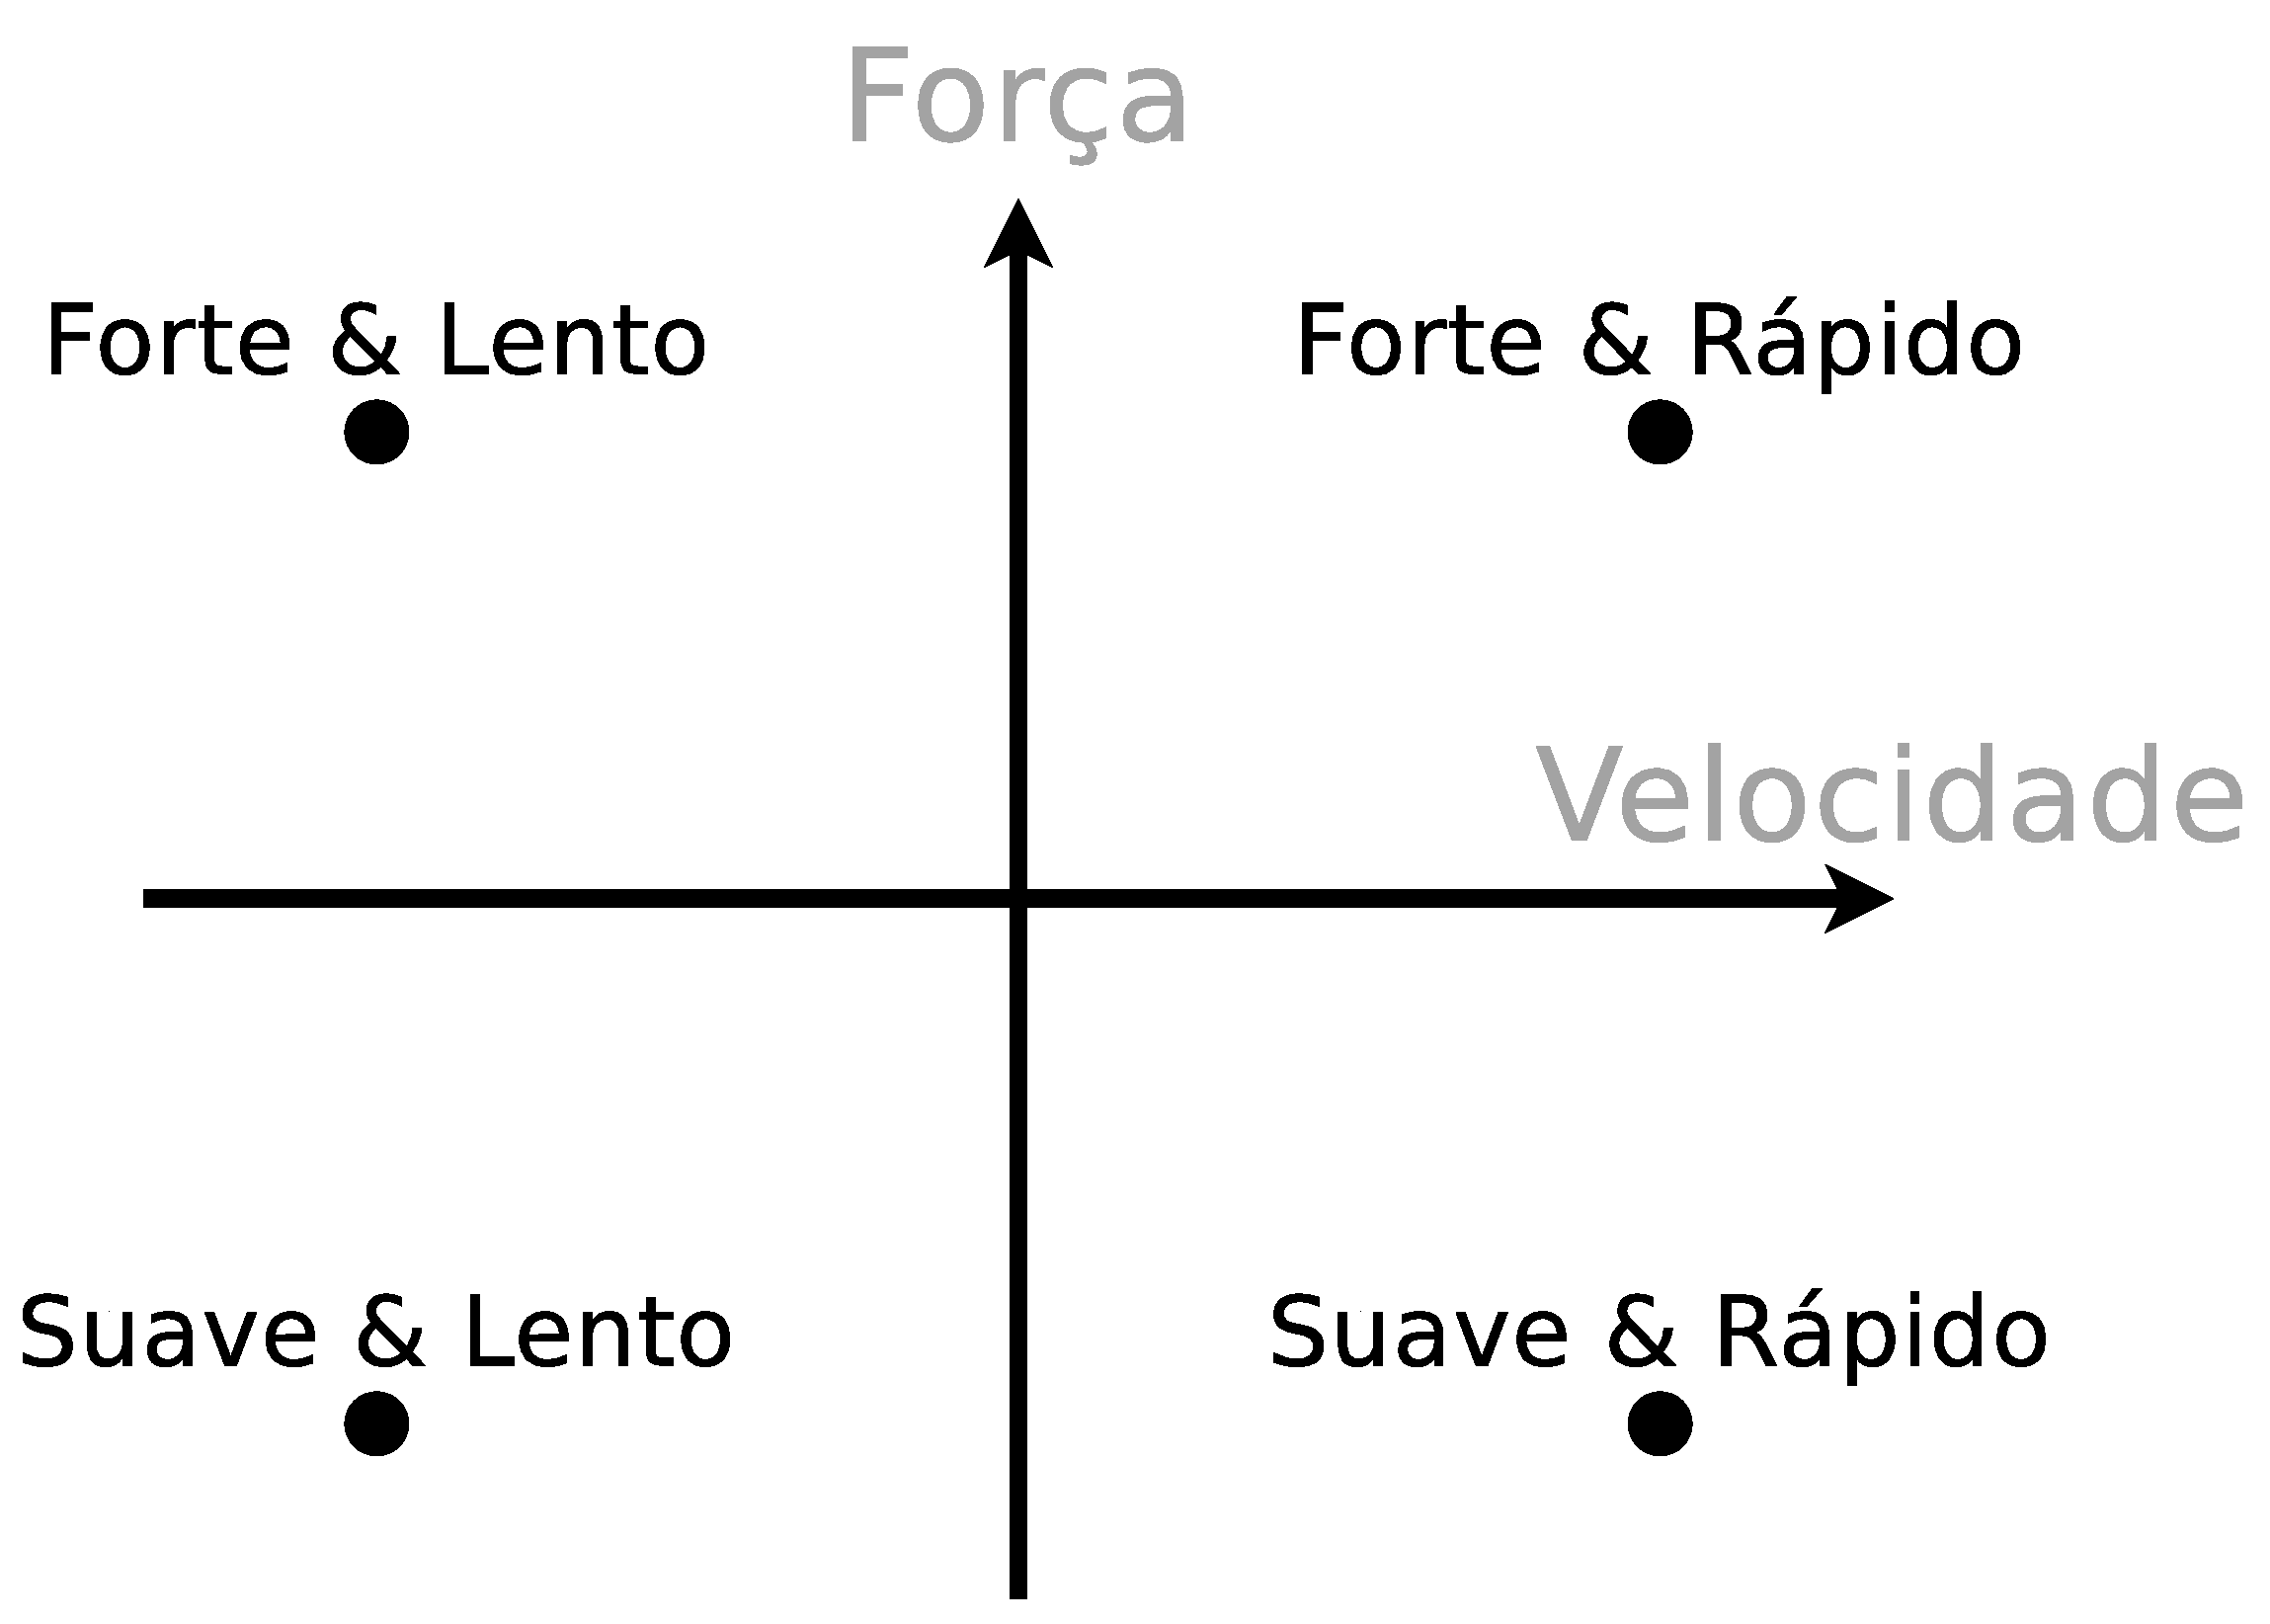
\includegraphics[width=0.45\textwidth]{chapters/cap-musicalidade/dinamicas-elementos2.eps}
\caption{Combinando elementos.}
\label{fig:element:moviment2}
\end{figure}

\begin{example}[Treino de ``Lady style'':]
\index{Lady style}
No treinamento de enfeites femininos (também conhecido como ``lady style'')
é possível observar a importância do uso das dinâmicas;
por exemplo, se escolhemos um movimento, 
como levantar os braços e logo descer eles (como quando o seguidor faz um giro).
Podemos observar uma variedade de texturas do movimento,
modificando os parâmetros  \{F,V,C\} nas dinâmicas.
\begin{itemize}
\item Os braços podem subir e descer fazendo um movimento continuo, leve e lento.
\item Os braços podem subir num movimento forte e rápido,
e com uma transição continua descer os braços de forma leve e lenta.
\item Os braços podem subir leve e lento,
e com uma transição continua descer os braços com tensão muscular e rápida 
(explosivo com arrumada ou desarrumada de cabelo). 
\item Etc.
\end{itemize}
\end{example}

%%%%%%%%%%%%%%%%%%%%%%%%%%%%%%%%%%%%%%%%%%%%%%%%%%%%%%%%%%%%%%%%%%%%%%%%%%%%%%%%
\subsection{Fatores do movimento: Um modelo simplificado}

\begin{wrapfigure}{r}{0.6\textwidth}
\centering
\smartdiagramset{
  text width=5.5cm,
  module minimum width=3.5cm,
  module minimum height=1.5cm
} 
\smartdiagram[bubble diagram]{Fatores do\\movimento,Energia,Continuidade}
\caption{Fatores do movimento num modelo simplificado.}
\label{fig:fatores:moviemnto:simplificada}
\end{wrapfigure}
Seguindo alguns profissionais  da dança, 
as dinâmicas do movimento nos indicam a forma em que a energia do corpo
é gastada, liberada ou modulada na dança \cite[pp. 126, 131, 136]{mccutchen2006teaching}.

Podemos usar a energia em vários níveis de intensidade ou estágios,
sendo que o uso da energia envolve também o uso de vários níveis de intensidade 
nos fatores velocidade e força, vistos na Seção  \ref{subsec:fator:movimento:atual} \cite[pp. 99]{sofras2019dance}.

Seguindo o coreografo e dançarino, Alonzo King \cite[pp. 99, 100]{sofras2019dance}:
\begin{citando}%%
Energia é a textura entre os movimentos.
Os movimentos falam com os dançarinos.
Estados físicos criam estados emocionais.
\end{citando}
Alonzo também indica que a energia usada nos movimentos,
 cria frases de dança com significado e dimensão \cite[pp. 99]{sofras2019dance}.

\begin{FraseFernandoPR}
Algumas vezes você tem que \hyperref[ref:emotionsentimental]{\textbf{sentir-se}} feliz para poder sorrir,
porém outras vesses você terá que sorrir para poder chegar a sentir-se feliz. %(2018-03-30)
\end{FraseFernandoPR}

A energia pode ser usada para contrair ou tensionar os músculos,
movimentar-nos rapidamente ou lenta e controladamente, pular, 
ou para conter e segurar nossa inercia gerando uma mudança abruta no fluxo da energia.

Assim, 
uma forma muito simplificada de iniciar as pessoas a trabalhar no uso das dinâmicas do movimento,
é separando as nossas dinâmicas em dois fatores:
\begin{description}
\item[Energia] (Baixo nível de energia $\rightarrow$ Alto nível energia)
Refere-se a quantidade de energia que gastamos em realizar nosso movimento;
este pode estar em algum ponto intermediário entre dois níveis de energia. 
O uso da energia, como fator de movimento, embrulha num só fator os 
fatores velocidade e força vistos na Seção  \ref{subsec:fator:movimento:atual}.
\item[Continuidade:] (Continuo $\rightarrow$ abrupto)
Este fator de movimento é o mesmo que vimos na Seção \ref{subsec:fator:movimento:atual};
refere-se ao grau de continuidade ao realizar nossos movimentos;
onde podemos escolher valores de continuidade em algum ponto intermediário entre continuo e abrupto.
\end{description}~

\begin{example}[Explorando o uso de níveis de energia:]
Podemos estudar a energia de nossos movimentos fazendo um pequeno exercício,
primeiro escolheremos um movimento, por exemplo: estirar os braços.
e depois usaremos 3 diferentes níveis de energia para executar este movimento;
por exemplo: baixa, meio ou alto nível de energia.
\end{example}

%%%%%%%%%%%%%%%%%%%%%%%%%%%%%%%%%%%%%%%%%%%%%%%%%%%%%%%%%%%%%%%%%%%%%%%%%%%%%%%%
\subsection{Dinâmica: Força - Tensão e Relaxação }
\label{sec:musicalidadetensionrelease}

% Bryan Adams - Summer Of '69 
%https://tabs.ultimate-guitar.com/tab/bryan_adams/summer_of_69_chords_843137

% https://books.google.com.br/books?id=PZdnDTxLscIC&pg=PA7&lpg=PA7&dq=tension+%2B+release+%2B+dance&source=bl&ots=c42uHzTXla&sig=ACfU3U1lZmDB5Jd23e41icQQKpzUnea0nw&hl=pt-BR&sa=X&ved=2ahUKEwj2-qz4ha3kAhUsIbkGHdRyBQgQ6AEwEnoECAgQAQ#v=onepage&q=tension%20%2B%20release%20%2B%20dance&f=false

Como vimos nas seções anteriores,
um dos fatores do movimento é a ``força'', 
ou o ``peso'' no modelo de Laban,
sendo que este fator pode ter valores entre dois extremos,
que nesta seção chamaremos como, ``relaxação'' e ``tensão''.
Este fator é muito usado, 
devido a que nós controlamos nossos movimentos corporais 
mediante um balance entre a tensão e a relaxação muscular \cite[pp. 7]{schrader2005sense}.

Quando queremos explorar o fator força em nossa dança, tentaremos na medida do possível,
manter os outros fatores como velocidade e continuidade em valores intermediários,
para que o protagonismo no movimento seja para o fator força,
que será usado modificando seu valor desde a relaxação ate a tensão, e vice-versa, no transcurso dos movimentos. 

Como vimos na Seção \ref{sec:tensionrelease}, 
ao escutar música comumente percebemos ciclos de tensão e relaxação,
provocadas por dissonâncias,  cadências nas frases musicais, ou mudanças de
tom, intensidade, ritmo, etc.
Assim, 
seguindo o explicado sobre o \hyperref[sec:interpretacioncorporal]{\textbf{mapeamento}}\footnote{Para
ver o tema do mapeamento de aspectos da música ir a Seção \ref{sec:interpretacioncorporal}.} 
de aspectos da música e aspectos do movimento,
podemos associar a tensão e relaxação dos movimentos de nossa dança à música.



\begin{description}
\item[Tensão muscular:] Para gerar tensão, 
deveremos realizar nossos movimentos aumentado o grau de ativação muscular (contração muscular, aspecto de potencia), 
seguindo nossa imaginação e  critério;
para projetar uma imagem, por exemplo, de que estamos suportando tensão (como quando puxado por uma corda), 
peso (como um andar carregando um objeto pesado), força (como empurrando um objeto pesado), etc.
Para mais detalhes sobre ativação muscular ver os  Exemplos \ref{ex:tension:on}, \ref{ex:tension:on2} e \ref{ex:tension:on3}.
\begin{example}[Ativação muscular no esforço:]
\label{ex:tension:on}
Imaginemos que debemos mexer nossa mão 30 cm a direita, em 3 segundos;
porém, na primeira tentativa, nos temos que arrastrar com essa mão um pacote de 5Kg,
e na segunda vez não.
É evidente que, tendo em ambos casos a mesma velocidade e percorrido,
no primeiro a nossa ativação muscular será superior que no segundo caso.
\end{example}
\begin{example}[Ativação muscular do carateca:]
\label{ex:tension:on2}
Imaginemos a um carateca realizando seus treinamentos de forma unipessoal, 
fazendo sombra; é dizer, lutando com um oponente imaginário;
nesse instante mesmo sem fazer contato físico com seu adversário,
ele está com uma elevada ativação muscular em cada golpe,
sendo esta caraterística evidente para qualquer  observador.
\end{example}
\begin{example}[Ativação muscular do mimo:]
\label{ex:tension:on3}
Outra forma de ver ativação muscular é quando assistimos a apresentação de um mimo,
e ele faz os movimento de  abrir uma porta e carregar ou empurrar um objeto;
não só reproduzindo a trajetória dos movimentos, 
se não que também incorporando a ativação muscular necessária que teria o movimento. 
\end{example}
\item[Relaxação muscular:] Para gerar relaxação, 
deveremos realizar nossos movimentos, 
de modo que seja  perceptível para nós um movimento predominantemente ósseo\footnote{Esta
descrição é para estar no extremo da relaxação.}, 
que um movimento por ativação muscular;
é evidente que todo movimento tem ativação muscular,
porém na relaxação esta caraterística não é o protagonista,
e sim o movimento ósseo.
\begin{example}[Relaxação da marionete:]
Imaginemos uma marionete controlada por fios, 
onde podemos observar o movimento relaxado do boneco.
A marionete se movimenta sem ativação muscular, 
e só percebemos nele o movimento ósseo de suas extremidades, 
contido só pelas suas articulações.

Assim, a maneira de treinamento, 
podemos tentar movimenta-nos imitando os movimentos de uma marionete,
para poder entender como é um corpo com relaxação extrema,
e como incorporar esta caraterística dosificadamente em nossos movimentos de dança.
\end{example} 
\end{description}

~

\PRLsep{Break aplicando tensão e relaxação}
\index{Musicalidade!Break}

Uma forma de aproveitar os \hyperref[sec:UsandoBreak]{\textbf{breaks}} na música,
é criando dinâmicas de tensão e relaxação.
Isto é, criar tensão  no nosso corpo quando o break está a ponto de estourar,
e relaxação no silencio provocado quando o break estourou,
como é mostrado na Figura \ref{fig:tension-release-climax}.
O quanto tempo usemos para acumular tensão e para liberar-lha 
é uma escolha criativa de cada um, 
limitado unicamente pelo tempo que disponhamos;
por exemplo, o tempo de silencio num break geralmente é curto.



\begin{figure}[!h]
  \centering
    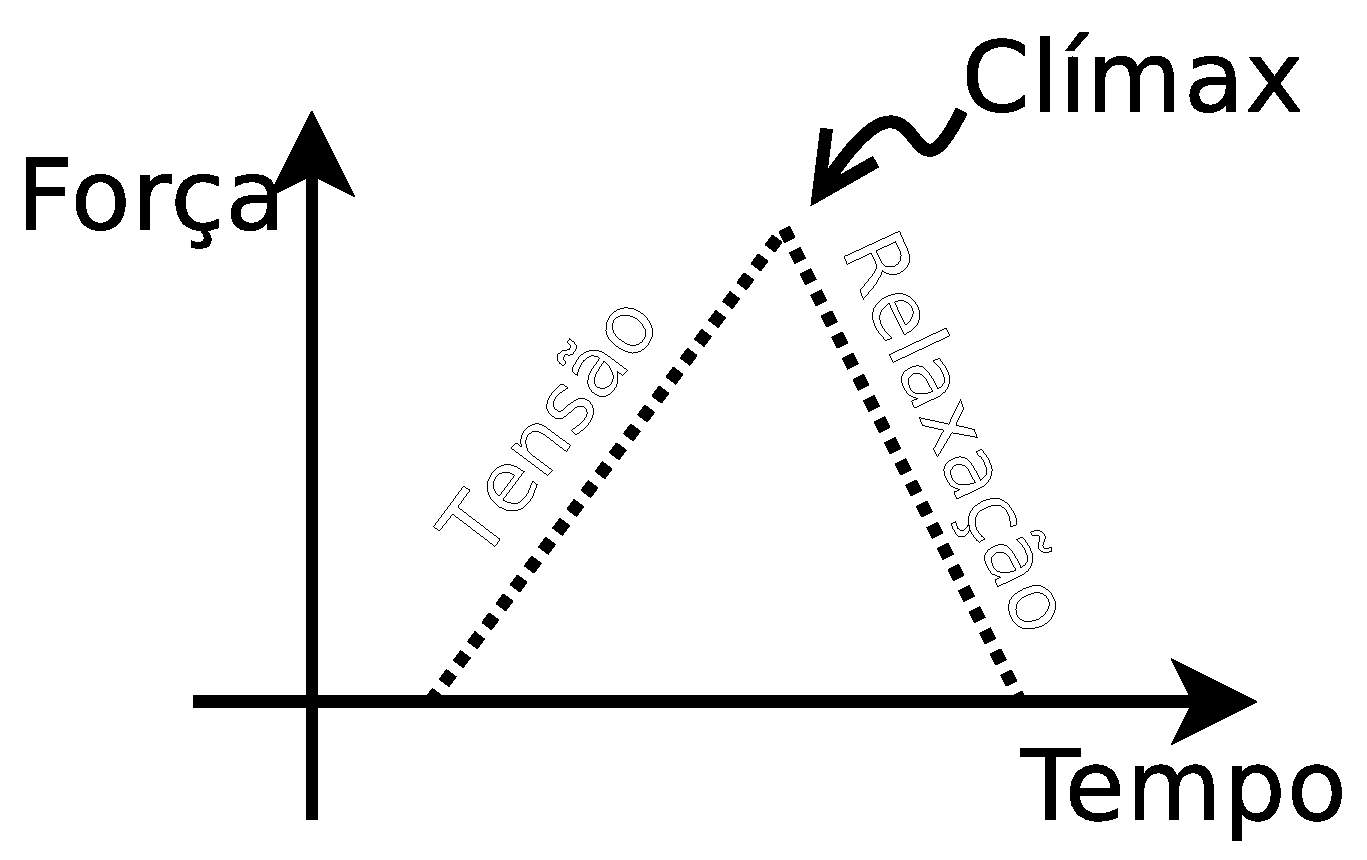
\includegraphics[width=0.5\textwidth]{chapters/cap-musicalidade/tension-release-climax.eps}
\caption{Uso do \hyperref[ref:climax]{\textbf{clímax}} na dinâmica de tensão e relaxação.}
\label{fig:tension-release-climax}
\end{figure}


\PRLsep{Dança a dois aplicando tensão e relaxação}

Podemos aproveitar a dinâmica da tensão e relaxação na dança a dois,
já seja de forma unipessoal ou como trabalho de par,
a continuação são listadas algumas dicas.
\begin{itemize}
\item Se o condutor está com um abraço fechado de dança, 
é possível aproveitar a mudança de tensão a relaxação da música,
criando tensão muscular nosso último movimento antes do \hyperref[ref:climax]{\textbf{clímax}} na música,
para logo paulatinamente voltar a uma relaxação muscular,
dando um efeito de mola que estica e encolhe,
para qualquer de nossos movimentos.
\item Se estamos com um abraço de dança aberto, ou estamos dançando separados de nosso par,
qualquer pessoa do par de dança pode aplicar a tensão e relaxação muscular, 
no seu próprio corpo de maneira independente, possivelmente gerando uma posse,
e voltando a relaxação, ou estendendo o último movimento realizado na dança,
em qualquer caso o efeito visual será parecido a uma mola que se tensiona e logo se relaxa.
\end{itemize}



%%%%%%%%%%%%%%%%%%%%%%%%%%%%%%%%%%%%%%%%%%%%%%%%%%%%%%%%%%%%%%%%%%%%%%%%%%%%%%%%
%https://translate.google.com.br/translate?sl=en&tl=pt&u=https%3A%2F%2Fblog.steezy.co%2Fwhat-are-textures-in-dancing%2F
\subsection{Dinâmica: Continuidade - Legato e sttacato }
\index{Musicalidade!Articulação}
\index{Musicalidade!Continuidade}
\index{Musicalidade!Legato}
\index{Musicalidade!Sttacato}


O fator do movimento ``continuidade'', 
ou ``flow'' em inglês, tem valores entre dois extremos: continuo e  abrupto.
Na maioria das vesses quando dançamos estamos num valor intermédio de continuidade,
sem aproveitar demasiado os extremos.
Assim, quando desejamos explorar este fator, manteremos na medida do possível,
os outros fatores como velocidade e força em valores intermediários,
para assim poder ressaltar a continuidade.

Como vimos na Seção \ref{sub:Articulation}, 
ao escutar uma música percebemos que existem formas de \hyperref[sub:Articulation]{\textbf{articular}} as notas musicais;
por exemplo, estas podem ser articuladas em 
\hyperref[subsec:Legato]{\textbf{legato}} ou \hyperref[subsec:Staccato]{\textbf{staccato}};
e dizer, as notas podem ser executadas consecutivamente sem emendas ou 
estas podem ser executadas de modo que seja claro onde inicia uma nota musical e onde termina a outra.
Assim, 
seguindo o explicado sobre o \hyperref[sec:interpretacioncorporal]{\textbf{mapeamento}}\footnote{Para
ver o tema do mapeamento de aspectos da música ir a Seção \ref{sec:interpretacioncorporal}.} 
de aspectos da música e aspectos do movimento,
podemos associar as articulações da música à dinâmica de continuidade nos movimentos de nossa dança.\\


\begin{description}
\item[Continuo:] Para gerar continuidade em nossos movimentos,
estes não devem ter emendas nem pausas; 
podem existir claro mudanças de velocidade e direção,
porém estas devem ser graduais e sutis.
\begin{example} 
Na Figura \ref{fig:continudade-all} temos umas curvas que representam uma metáfora de nossos movimentos,
onde os círculos indicam o inicio de cada movimento.
\begin{itemize}
\item Na Figura \ref{fig:continudade-a} vemos movimentos que são realizados de forma continua, 
em toda extensão destes, 
e inclusive a continuidade se conserva quando passamos de um tipo de movimento a outro.
\item Na Figura \ref{fig:continudade-b} vemos movimentos que são realizados de forma continua, 
em toda extensão destes;
porém a  continuidade se perde quando passamos de um tipo de movimento a outro.
\item Na Figura \ref{fig:continudade-c} vemos movimentos que são realizados de forma continua e linear,
diretos e sem movimentos desnecessários em toda extensão destes;
a continuidade é perdida quando passamos de um tipo de movimento a outro.
\end{itemize}
\end{example}

\item[Abrupto:] Para gerar descontinuidade em nossos movimentos, 
podemos eles realizando mudanças abruptas de direção, velocidade ou força,
de modo que seja evidente para qualquer observador cada tramo de nossos movimentos.
\begin{example}
Na Figura \ref{fig:continudade-all} temos umas curvas que representam uma metáfora de nossos movimentos,
onde os círculos indicam o inicio de cada movimento.
\begin{itemize}
\item Na Figura \ref{fig:continudade-d} vemos movimentos que são realizados de forma abrupta ou descontinua,
em toda extensão destes, 
e inclusive quando passamos de um tipo de movimento a outro.
\item Nas Figuras \ref{fig:continudade-b} e \ref{fig:continudade-c} 
vemos movimentos que só são descontínuos e abruptos nas emendas entre movimentos. 
\end{itemize}
\end{example}
\end{description}

\begin{figure}[!h]
     \centering
     \begin{subfigure}[b]{0.4\textwidth}
         \centering
         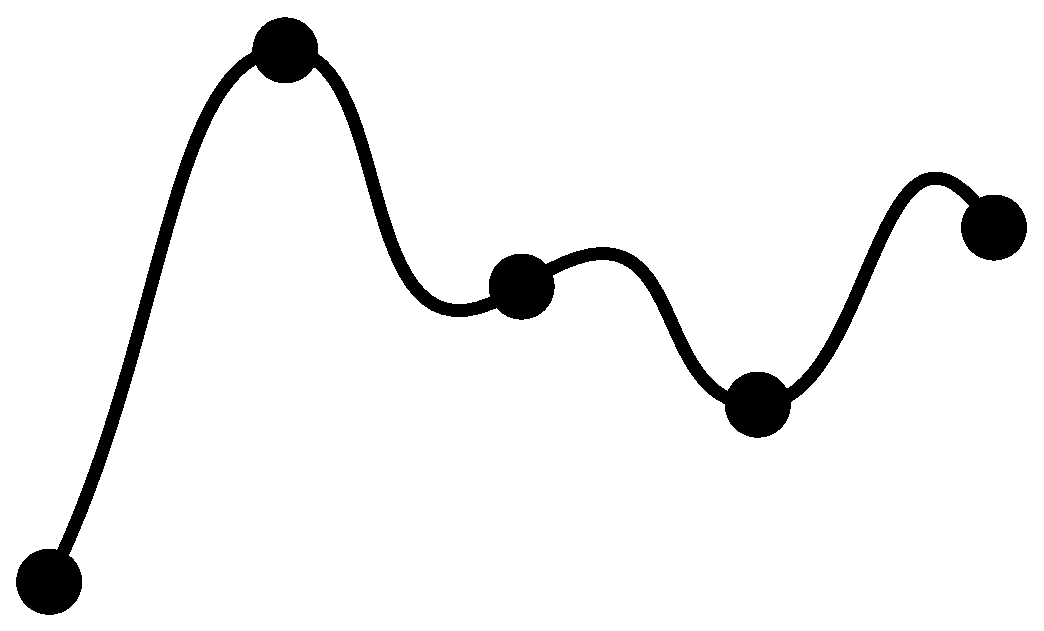
\includegraphics[width=0.8\textwidth]{chapters/cap-musicalidade/continudade-a.eps}
         \caption{Continuo no percorrido e emendas.}
         \label{fig:continudade-a}
     \end{subfigure}
     \hfill
     \begin{subfigure}[b]{0.4\textwidth}
         \centering
         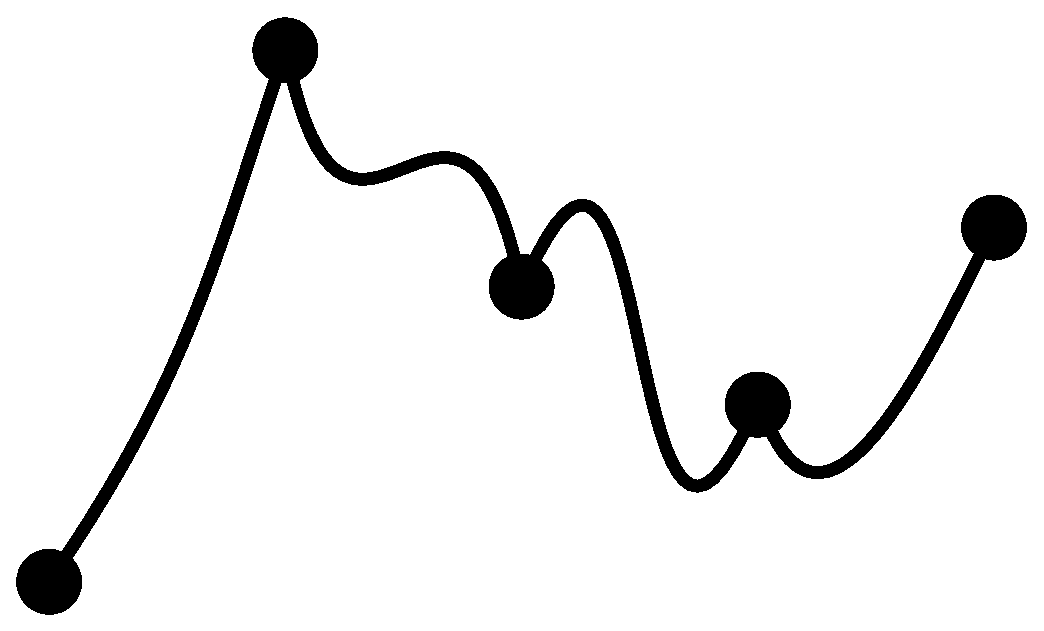
\includegraphics[width=0.8\textwidth]{chapters/cap-musicalidade/continudade-b.eps}
         \caption{Continuo no percorrido e abrupto nas emendas.}
         \label{fig:continudade-b}
     \end{subfigure}
     \hfill
     \begin{subfigure}[b]{0.4\textwidth}
         \centering
         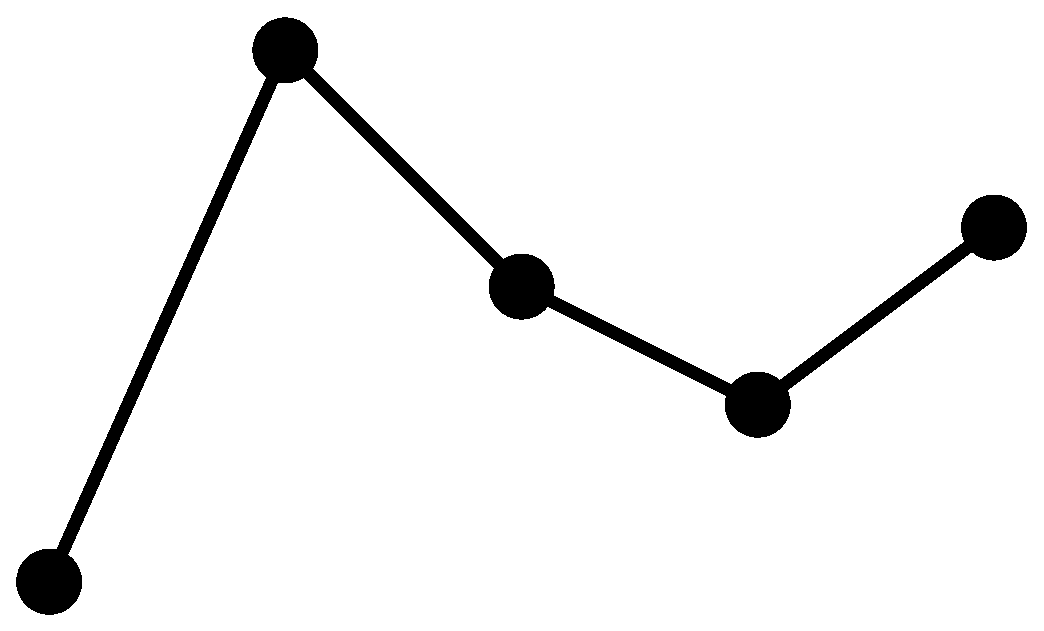
\includegraphics[width=0.8\textwidth]{chapters/cap-musicalidade/continudade-c.eps}
         \caption{Continuo linear no percorrido e abrupto nas emendas.}
         \label{fig:continudade-c}
     \end{subfigure}
     \hfill
     \begin{subfigure}[b]{0.4\textwidth}
         \centering
         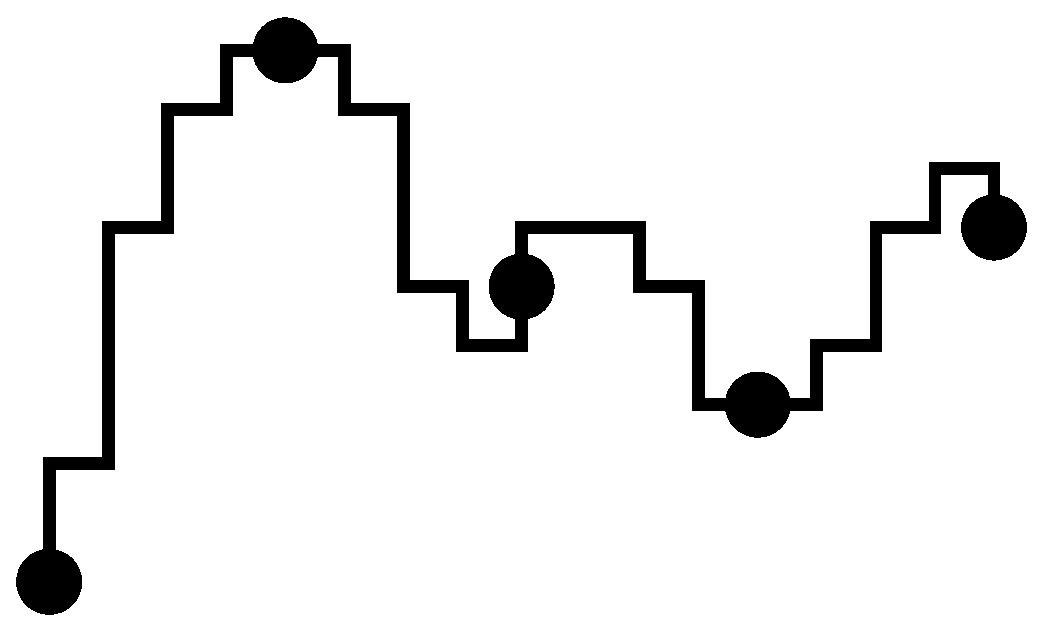
\includegraphics[width=0.8\textwidth]{chapters/cap-musicalidade/continudade-d.eps}
         \caption{Abrupto no percorrido e emendas.}
         \label{fig:continudade-d}
     \end{subfigure}
\caption{Usos do fator de movimento: continuidade.}
\label{fig:continudade-all}
\end{figure}

\begin{example}[Samba funkeado:]
Um exemplo interessante de movimentos abruptos nas emendas, 
é no estilo de dança \hyperref[subsec:sambafunkeado]{\textbf{samba funkeado}},
onde os movimentos tem continuidade na sua extensão, tendendo a ser rápidos no final,
para chegar a ter mudanças abruptas e marcadas para indicar o final de um movimento e o inicio de outro.
\end{example}

\PRLsep{Dançando em legato ou staccato}
Para aproveitar as articulações da música, como o legato e sttacato,
podemos usar as seguintes recomendações.\\
\begin{description}
\item[Malandragem:] Uma forma de criar movimentos que deem aparência de malandragem,
é realizando passos com mudanças abruptas nas emendas.
Por exemplo, quando a pessoa da um passo, 
este poderia chegar com o 100\% do peso do corpo no pé que movimentou.
Este efeito pode ser conseguido se ao dar esse passo:
\begin{itemize}
\item Nos imaginamos que levamos o peso do corpo para adiante, desde o quadril,
e quando não consigamos mais estar em equilíbrio, 
damos um passo ao frente para chegar a um novo equilíbrio.
\item Também podemos imaginar-nos, 
que nos deslocamos  andando por efeito de que algo nos puxa da cintura,
de modo que o quadril avança e logo o pé atua e obedece.
\end{itemize}
Esta forma de movimentar-se tem mudanças abruptas nas emendas,
como as metáforas presentadas nas Figuras \ref{fig:continudade-b} e  \ref{fig:continudade-c},
e pode ser mapeado a mudanças abruptas na execução de notas musicais,
como no staccato.



\item[Elegância:] Podemos imitar as caraterísticas dos movimentos em danças como o bolero ou o tango,
onde antes de levar o peso do corpo, 
a pessoa primeiro leva o pé na posição desejada sem carregar o peso do corpo,
e logo paulatinamente, e pela ação do quadril, leva o peso do corpo a esse pé;
dando assim ao movimento um aspecto elegante como se a pessoa flutua-se.\\
Esta caraterística flutuante e continua do movimento, 
pode ser mapeada a mudanças de notas musicais em legato,
para ter correlação entre a música e o movimento.
\end{description}~

De forma geral, 
nossa dança pode se encontrar em algum ponto intermediário entre as dinâmicas que provocam elegância ou malandragem, 
como mostra a Figura \ref{fig:malandragem-elegancia},
a escolha dependerá exclusivamente da decisão artística de cada dançarino,
e a relação que estos decidam guardar com a música.
\begin{figure}[!h]
  \centering
    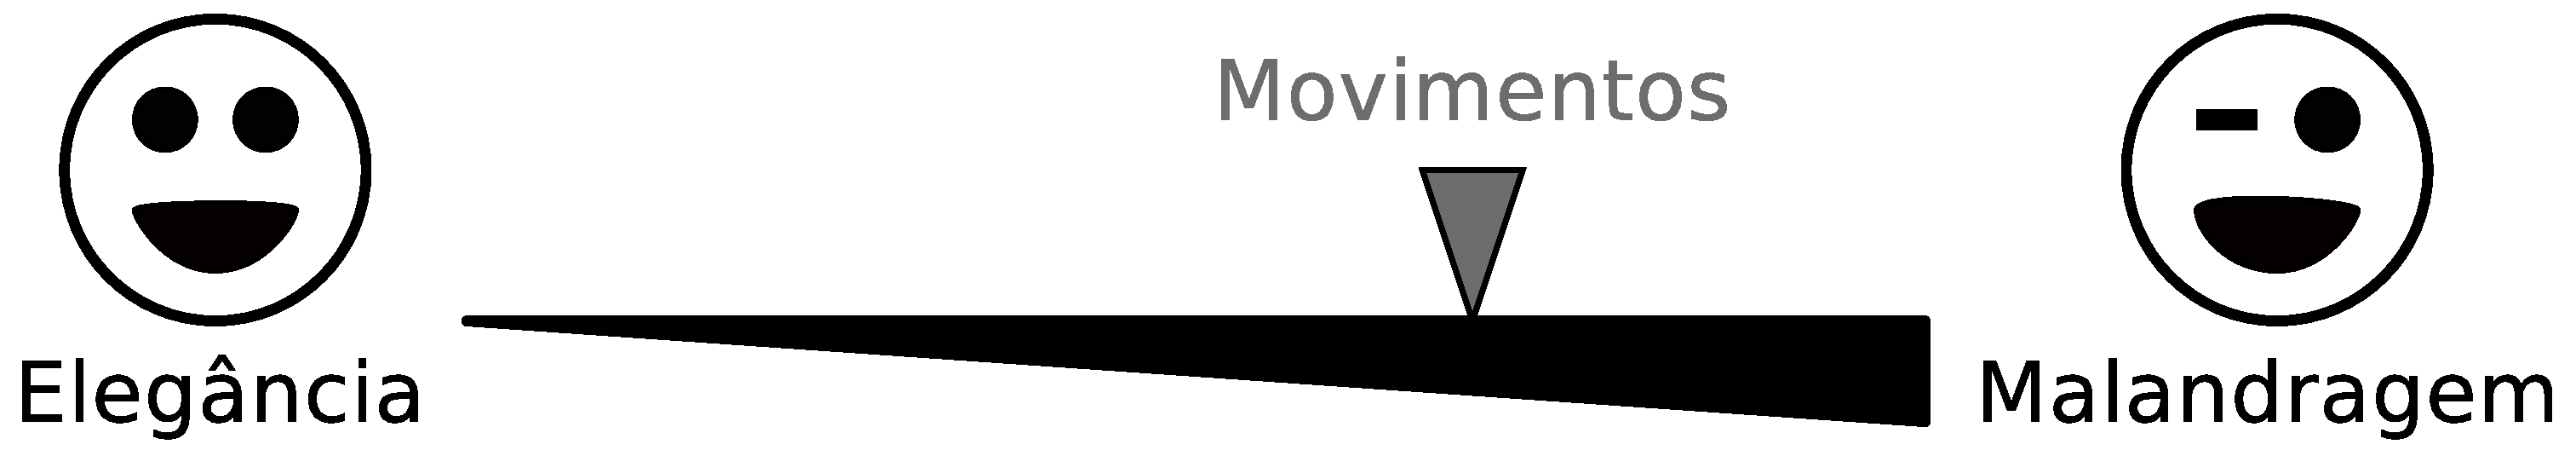
\includegraphics[width=0.65\textwidth]{chapters/cap-musicalidade/malandragem-elegancia.eps}
\caption{Malandragem e elegância.}
\label{fig:malandragem-elegancia}
\end{figure}


%%%%%%%%%%%%%%%%%%%%%%%%%%%%%%%%%%%%%%%%%%%%%%%%%%%%%%%%%%%%%%%%%%%%%%%%%%%%%%%%
\subsection{Dinâmica: Velocidade }
\label{subsec:dinamica:velocidade}
\index{Musicalidade!Velocidade}


Podemos achar o fator do movimento, ``velocidade'', entre dois extremos: lento e  rápido.
Como foi mencionado nos casos anteriores, 
na maioria das vesses, 
quando dançamos desaproveitamos o fator velocidade usando só um valor intermédio,
variando  pouco ao redor deste valor.
Assim, uma forma de treinar a velocidade seria manter, na medida do possível,
os outros fatores como continuidade e força em valores intermediários,
para assim trabalhar levando a velocidade a seus extremos em nossas dinâmicas.

Não devemos esquecer que a velocidade (v) está relacionada com a distancia percorrida (d) e o tempo (t),
mediante a Equação \ref{eq:vdt}.
\begin{equation}
\label{eq:vdt}
v=\frac{d}{t}
\end{equation}
Assim, 
uma forma de alterar a velocidade é modificar coerentemente o percorrido ou a duração do movimento.


\begin{description}
\item[Lento:] Neste caso nossos movimentos terão uma velocidade abaixo da media.
Para diminuir a velocidade podemos tomar dois caminhos.
\begin{itemize}
\item O primeiro seria manter constante a distancia do percorrido de nosso movimento,
e aumentar o tempo que empregamos para realizar este.
\item O segundo seria manter constante a duração do movimento e diminuir a distancia percorrida por este. 
\end{itemize}
\item[Rápido:] Por oposição ao caso anterior, 
aqui nossos movimentos estarão acima da media.
Para aumentar a velocidade podemos tomar dois caminhos.
\begin{itemize}
\item O primeiro seria manter constante a distancia do percorrido de nosso movimento,
e diminuir o tempo que empregamos para realizar este.
\item O segundo seria manter constante a duração do movimento e aumentar a distancia percorrida por este. 
\end{itemize}
\end{description}

\begin{example}[Treinando mantendo constante o tempo:]
Para este treinamento devemos escolher uma música, por exemplo uma em compasso binário,
identificar o tempo forte e fraco, e logo executar nossos movimentos em cada tempo,
de modo que o único que podemos modificar em nossas dinâmicas seja a distancia percorrida,
e consequentemente a velocidade da dinâmica, que estará em função de algum aspecto da música.
Uma possível escolha de movimento seria dar passos a alguma direção.
\end{example}

\begin{example}[Treinando mantendo constante a distancia:]
Para este treinamento devemos realizar movimentos com o mesmo percorrido,
e modificar o tempo que utilizamos para executar ele, 
de modo que indiretamente modifiquemos a velocidade da dinâmica.

Assim, para este treino devemos fazer marcas equidistantes, fisicamente ou mentalmente, 
sobre uma superfície, 
e interpretaremos uma música só movimentando-nos de uma marca a outra,
de modo que seja o tempo do percorrido o único fator que modifiquemos.
\end{example}


\begin{example}[Velocidade constante no ``tchic tchic tum'':]~

\begin{abc}[name=abc-veltchictchictum,width=0.38\textwidth]
X: 1 % start of header
K: C stafflines=1 % scale: C major
M: 2/4 %meter - compasso
%Q:1/4=80
V:1 clef=perc stem=up %name="Pauta com clave de fá"   sname="Pauta com clave de fá"
[V:1] |: B2 B1 B1:|
w: tum tchic tchic
\end{abc}

Um treinamento interessante para desenvolver o contro corporal,
pode ser feito utilizando uma sequencia rítmica  ``tchic tchic tum''.
Neste caso tentaremos manter uma velocidade constante em nosso andar,
enquanto nossos pés executam passos com cada som, já seja um ``tchic'' ou um ``tum''.

Observem que o tempo de nossos movimentos é fixo e definido pela sequencia rítmica,
porém este é irregular, tendo um tempo de reação dobrado para o movimento apos ``tum'',
que para os movimentos apos um ``tchic''.
Assim, com essa distribuição irregular de tempos, 
devemos também ter uma distribuição  irregular de distancias de percorrido,
para poder manter constante a velocidade de nosso movimento.
\end{example}
%: ``slow motion'' e velocidade aumentada




%%%%%%%%%%%%%%%%%%%%%%%%%%%%%%%%%%%%%%%%%%%%%%%%%%%%%%%%%%%%%%%%%%%%%%%%%%%%%%%%
\subsection{Dinâmica: Energia }
\label{sec:musicalidadenergia}
O fator do movimento ``energia'', 
tem níveis  que vão entre dois extremos: baixa e alta energia.
Nos seguintes exercícios, quantificaremos esta faixa de energia em só 3 neveis,
que usaremos para mostrar texturas em nossos movimentos.

\begin{figure}[!h]
  \centering
    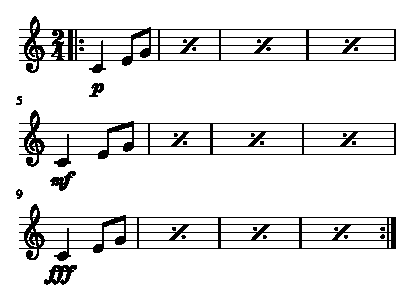
\includegraphics[width=0.8\textwidth]{chapters/cap-musicalidade/dinamica-energia-1.eps}
\caption{Ritmos usando 3 distintos matizes nas dinâmicas.}
\label{fig:dinamica-energia-ex1}
\end{figure}

\begin{example}[Usando 3 níveis de energia: sem deslocamento]
Para realizar este exercício, escolheremos um movimento; como por exemplo,
pisar no lugar, com um pé por vez, 
e com nosso movimento  acompanharemos nota por nota 
ao ritmo descrito na pauta da Figura \ref{fig:dinamica-energia-ex1}.
\begin{itemize}
\item Quando o ritmo tenha um matiz ``piano'' (\textbf{\textit{p}}) 
usaremos um movimento com suave,
com pouca força e quase sem movimentar-nos.
\item Quando o ritmo tenha um matiz ``mezzo forte'' (\textbf{\textit{mf}}) 
usaremos um movimento que seja natural e cotidiano,
com uma força regular, movimentando-nos de forma relaxada.
\item Quando o ritmo tenha um matiz ``extremadamente forte''  (\textbf{\textit{fff}}) 
usaremos um movimento que seja exagerado,
com uma muita força com movimentos como atacando o chão.
\end{itemize}
\end{example}

\begin{example}[Usando 3 níveis de energia: com deslocamento]
Para realizar este exercício, escolheremos um movimento; como por exemplo,
dar um passo, com um pé por vez, 
e com nosso movimento acompanharemos nota por nota 
ao ritmo descrito na pauta da Figura \ref{fig:dinamica-energia-ex1}.
\begin{itemize}
\item Quando o ritmo tenha um matiz ``piano'' (\textbf{\textit{p}}) 
daremos um passo extremadamente curto e suave como se tivéssemos medo de quebrar o chão.
\item Quando o ritmo tenha um matiz ``mezzo forte'' (\textbf{\textit{mf}}) 
daremos um passo de andar natural, com uma força regular e um passo relaxado. 
\item Quando o ritmo tenha um matiz ``extremadamente forte''  (\textbf{\textit{fff}}) 
daremos passos muitos longos, com muita energia no nosso andar, 
procurando recorrer a maior distancia possível.
\end{itemize}
\end{example}

% %%%%%%%%%%%%%%%%%%%%%%%%%%%%%%%%%%%%%%%%%%%%%%%%%%%%%%%%%%%%%%%%%%%%%%%%%%%%%%%%
%%%%%%%%%%%%%%%%%%%%%%%%%%%%%%%%%%%%%%%%%%%%%%%%%%%%%%%%%%%%%%%%%%%%%%%%%%%%%%%%
\section{\textcolor{red}{Cadência na dança }}
\index{Musicalidade!Cadência}

\begin{definition}[Cadência] 
\index{Musicalidade!Cadência}
\label{def:cadencia}
O Dicionário Online de Português define cadência como \cite{diciocadencia}:
\begin{itemize}
\item Ritmo; sequência encadeada e regular de sons e de movimentos.
\item \textbf{Literatura} Harmonia na forma de pronunciar as palavras; ritmo das palavras, segundo a acentuação tônica de cada sílaba.
\item \textbf{Música} Sucessão de notas e de acordes que definem o tom.
\item \textbf{Música} Unidade abstrata que mede o tempo musical, marcando as relações de ritmo.
\end{itemize}
\end{definition}


%% 
%% https://books.google.com.br/books?id=s0yb-6BXp1wC&pg=SA6-PA18&dq=cadence+%2B+tango&hl=es-419&sa=X&ved=0ahUKEwivpbuYmdbjAhW-LLkGHUuEAncQ6AEILDAA#v=onepage&q=cadence&f=false



% %%%%%%%%%%%%%%%%%%%%%%%%%%%%%%%%%%%%%%%%%%%%%%%%%%%%%%%%%%%%%%%%%%%%%%%%%%%%%%%%
%%%%%%%%%%%%%%%%%%%%%%%%%%%%%%%%%%%%%%%%%%%%%%%%%%%%%%%%%%%%%%%%%%%%%%%%%%%%%%%%
\section{\textcolor{red}{Motif ou motivos na dança }}
\index{Musicalidade!Motivos}
\index{Musicalidade!Motif}

motif e olementos da dança proposto por Laban \cite[pp. 46]{paine2014complete}.

% https://books.google.com.br/books?id=WluhAwAAQBAJ&pg=PT189&dq=force+speed+continuity+dance&hl=pt-BR&sa=X&ved=0ahUKEwiX5LeYj87lAhU3G7kGHUYBBJcQ6AEINDAB#v=onepage&q=force%20speed%20continuity&f=false

\newpage
%%%%%%%%%%%%%%%%%%%%%%%%%%%%%%%%%%%%%%%%%%%%%%%%%%%%%%%%%%%%%%%%%%%%%%%%%%%%%%%%
%%%%%%%%%%%%%%%%%%%%%%%%%%%%%%%%%%%%%%%%%%%%%%%%%%%%%%%%%%%%%%%%%%%%%%%%%%%%%%%%
\section{Dançando no tempo forte e em contra do tempo forte}
\label{sec:dancandotempoforte}
\index{Musicalidade!Dançando no tempo forte}
\index{Musicalidade!Dançando no tempo fraco}

Nesta seção será proposto um modo de uso do termo
``dançar no tempo forte'' e
``dançar em contra do tempo forte'' ou seu equivalente 
``dançar a contratempo'' no contexto da dança;
neste último caso de uso, mostraremos a relação entre o uso achado na literatura mundial sobre dança,
e a definição de tempo e \hyperref[sec:contratempo]{\textbf{contratempo}} na literatura sobre música.

\subsection{Contratempo na dança espanhola}
\label{subsec:contratempoespanha}
No livro sobre dança espanhola, ``Compendio de las principales reglas del baile'' (1820) \cite[pp. 131]{cairon1820compendio},
podemos ver a descrição de passos denominados contratempos.
\begin{citando}
Se llaman \textbf{contratiempos} todos aquellos pasos en que estando colocado el cuerpo sobre un pie,
y teniendo el otro en el aire,
se salta sobre el que está en el suelo antes de colocar el otro en tierra;
\end{citando}
Assim, na dança espanhola de 1820 são conhecidos como contratempos,
movimentos em que se impulsa ou salta num pé e se pisa com o outro. 
A relação, na dança espanhola,  dos passos com pulos
com o contratempo na música 
é explicado na tese de doutorado titulada 
``La danza en España en la segunda mitad del siglo XVIII: El bolero'' (2017)
\cite[pp. 160]{martin2017danza} onde se menciona:
\begin{citando}
En el Amable de estilo italiano se ejecutaban pasos saltados muy complicados como el sisone,
asamblé, jeté, piruetas y diversidad de saltos executados en los \textbf{contratempos} musicales.
\end{citando}
É dizer, estos passos pulados eram executados nos contratempos musicais;
ou seja, acentuando mais um tempo fraco que o tempo forte,
ou acentuando mais a parte fraca do tempo que a parte forte deste;
de modo que estes saltos foram denominados a contratempo.
Podemos ver esta relação no livro ``Glosario de términos de la danza española'' (2001)
\cite[pp. 109]{aubero2001glosario}, onde mencionam:
\begin{citando}
Despues del <<salto mayor>>, cuando el bailarín salta en el aire en el $4^o$ tiempo,
puede caer sobre ambos pies juntos (a pie) o en <<contratiempo>>.
\end{citando}
Confirmando-nos que o pulo era feito num tempo fraco (quarto tempo).



\subsection{Contratempo na dança em cuba}
\label{subsec:contratempocuba}
No ``Diccionario de la música cubana'' (1981) 
\cite[pp. 113]{orovio1981diccionario} \cite[pp. 57]{santana2005merengue},
podemos achar o seguinte texto relativo às palavras do compositor e músico Enrique Jorrín.
\begin{citando}
Noté la dificultad de la mayoría en los ritmos sincopados, 
debido a que los pasos de los bailadores se producen a \textbf{contratiempo},
o sea en la segunda y cuarta corchea del compás de dos quartos.
\end{citando}
Assim, sabe-se que desde 1981 o músico Enrique Jorrín, 
já fazia uso de um paralelo entre o \hyperref[sec:contratempo]{\textbf{contratempo}} 
musical e um contratempo na dança;
seguindo suas palavras, de forma similar a o que temos na música, o contratempo na dança acontecia
quando o movimento\footnote{Se sobre entende que se refere ao movimento inicial do passo.} se executa no tempo fraco, 
no caso de um \hyperref[subsec:compassoquaternario]{\textbf{compasso quaternário}},
no segundo e quarto tempo;
se entende que é considerado o movimento inicial, ou principal, 
ao movimento acentuado num determinado passo de dança.
Esta suposição é corroborada no livro ``Historia del baile y la Rueda de Casino-Salsa'' (2012) \cite{borges2012historia},
onde se menciona que uma discussão, entre dançarinos e músicos,
é se a ``roda de casino'' se ``dança a tempo''\footnote{Se sobre entende que é o tempo forte.} 
e o ``son cubano'' a ``contratempo'',
ou vice-versa. E a continuação descreve que dançar a tempo
é dançar com o movimento inicial do passo básico no tempo 1 (tempo forte),
e dançar a contratempo é dançar com o movimento inicial do passo num tempo fraco, 
no caso do son cubano, iniciando no segundo tempo de um compasso quaternário.
Por outro lado, no livro ``Salsa y casino: de la cultura popular tradicional cubana'' (2010),
podemos achar outra descrição de dançar a contratempo \cite[pp. 63]{gutierrez2010salsa}.
\begin{citando}
Cuando el passo lateral se raliza a \textbf{contratiempo},
com relación a la clave del son,
el primer movimeinto del pie se hace abriendo lateralmente hacia afuera,
en el cuarto tiempo del compás.
\end{citando}
Ao igual que os casos apresentados anteriormente,
é chamado dança a contratempo a passos com o movimento inicial (principal) executado no tempo fraco,
neste caso o quarto tempo.

Outra explicação sobre dançar a contratempo, pode ser achada
no livro ``Spinning Mambo Into Salsa: Caribbean Dance in Global Commerce'' (2015) \cite[pp. 68]{mcmains2015spinning},
porem esta vez para o caso sincopado. 


%%%%%%%%%%%%%%%%%%%%%%%%%%%%%%%%%%%%%%%%%%%%%%%%%%%%%%%%%%%%%%%%%%%%%%%%%%%%%%%%
\subsection{Contratempo na dança no Brasil}
\label{subsec:contratempobrasil}
Na dança de salão no Brasil, 
o termo ``contratempo'' tem sido usado de forma informal por muitos profissionais da dança,
sendo o uso deste termo, em muitos casos, completamente desarraigado do seu significado musical,
constituindo em sim um neologismo semântico ou gíria.

\begin{definition}[Gíria:] 
\index{Gíria}
\label{def:Giria}
Podem ser achadas as seguintes acepções no Dicionário Priberam da Língua Portuguesa \cite{priberamgiria}:
\begin{itemize}
\item Linguagem característica de um grupo profissional ou sociocultural, é equivalente ao termo jargão.
\item Linguagem usada por determinado grupo, 
geralmente incompreensível para quem não pertence ao grupo e que serve também como meio de realçar a sua especificidade.
\end{itemize}
\end{definition}

\begin{definition}[Neologismo semântico:] 
\index{Neologismo!Neologismo semântico}
\label{def:NeologismoSemantico}
Um neologismo semântico ou neologismo de significado é caraterizado pela modificação 
do significado de uma palavra já existente na língua;
as gírias em muitas ocasiões constituem exemplos de neologismos semânticos, 
pois algumas gírias dão novos sentidos a palavras já usadas no vocabulário formal \cite[pp. 82-83]{correalingua}.
\end{definition}

No vocabulário informal do grupo profissional ou sociocultural da dança no Brasil,
é possível achar pelo menos, dois tipos de uso do termo contratempo.
\begin{itemize}
\item Em alguns casos é usada a palavra contratempo (CT) para indicar um lapso temporal, 
equivalente à metade de um tempo musical (T); é dizer: $CT=T/2$.
\item Em outros casos a palavra contratempo (CT) é usada para definir uma distribuição temporal 
ou ritmo da forma $\{T/2, T/2, T\}$; é dizer duas figuras musicais de duração $T/2$ e uma de duração $T$,
nessa ordem. De modo que neste uso, um contratempo tem uma duração temporal de $2T$
e um ``contrá'' tem uma duração temporal de $T/2$. 
\end{itemize}

Em qualquer dos dois casos anteriores, não podemos afirmar qual das duas acepções é correta,
pois pela sua natureza informal de ambas,
no melhor dos casos, só poderíamos indicar qual é a mais popular.

Nas minhas pesquisas de literatura de dança do Brasil, 
só tenho achado uma referencia bibliográfica que usa o termo contratempo para a dança;
no livro titulado ``Dança de salão: Uma alternativa para o desenvolvimento motor no ensino'' 
(2010) \cite{maia2010danca}.
Nesse texto não se explica o significado que se lhe da ao termo contratempo;
porem, pelo contexto pode-se intuir que se está usando a acepção informal 
que considera um contratempo como $T/2$, mas não se tem uma certeza.
A continuação se mostra o paragrafo antes mencionado:
\begin{citando}
Em uma mesma música, permite-se dançar passos diferentes em diferentes tempos,
que na dança de salão chama-se de passos no ``tempo'' ou no ``contratempo''.
\end{citando}


Em qualquer destes casos, 
estes usos do termo contratempo tem o problema principal, 
que estão completamente desarraigados do seu significado musical;
e geram confusões para pessoas que sim conhecem a definição formal de contratempo.
Assim observamos que criar um 
\hyperref[def:NeologismoSemantico]{\textbf{neologismo semântico}} com o termo contratempo, 
entre dois âmbitos tão próximos como a dança é a música, é uma fonte continua de confusões;
sobre tudo se pensamos, que as pessoas que estamos dedicadas ao estudo da dança,
somos as seguintes em interesse, apos os músicos, em aprender sobre teoria musical.


%%%%%%%%%%%%%%%%%%%%%%%%%%%%%%%%%%%%%%%%%%%%%%%%%%%%%%%%%%%%%%%%%%%%%%%%%%%%%%%%
\subsection{Que significa dançar no tempo forte?}
\index{Dançar no tempo forte}
\label{subsec:dancatempoforte}

\begin{wrapfigure}{r}{0.25\textwidth}
  \vspace{-10pt}
  \centering
    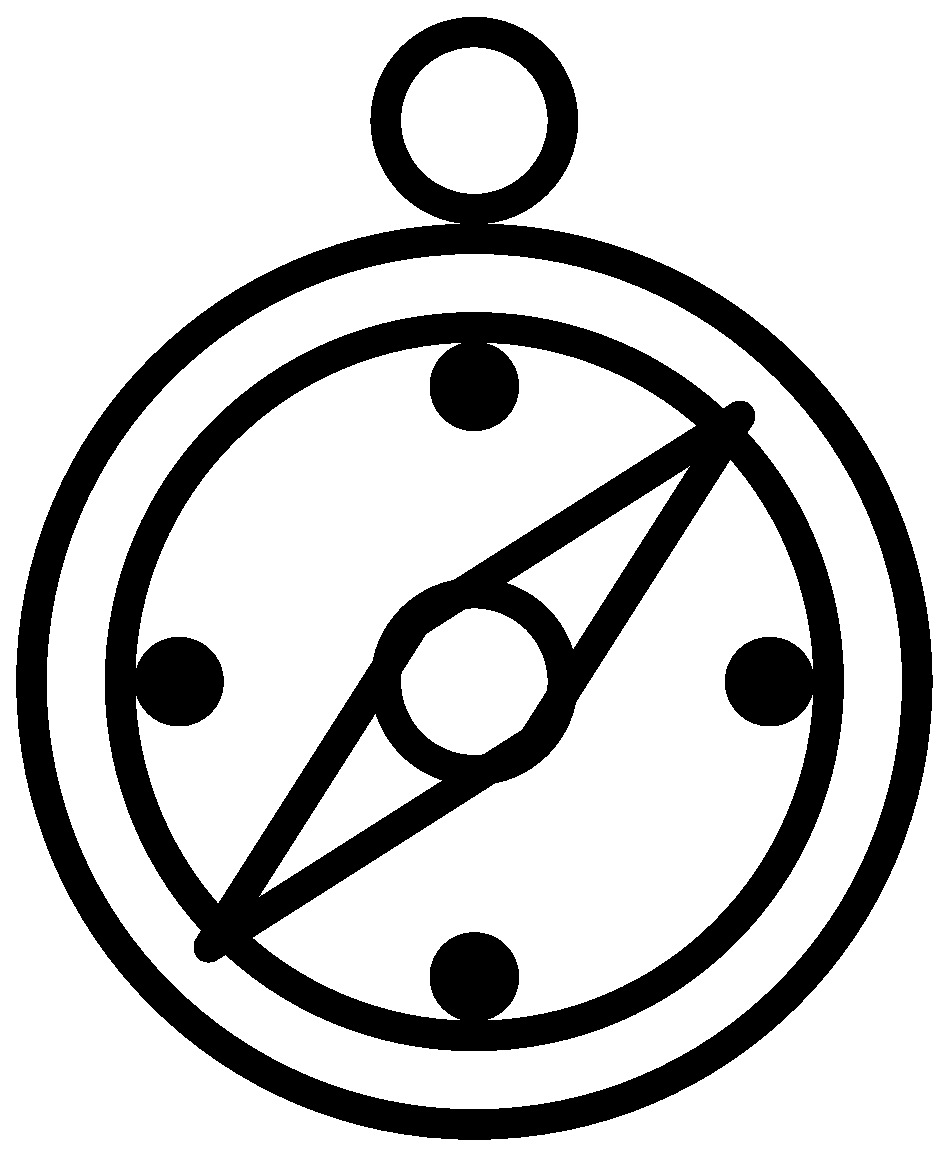
\includegraphics[width=0.2\textwidth]{compass.eps}
  \vspace{-10pt}
\end{wrapfigure}
Alguns professores de dança já usam a expressão ``dançar no tempo'', 
se referindo a ``dançar no tempo forte'', seguindo o mesmo sentido que já foi adiantado\footnote{Para 
ver a definição de dançar no tempo forte, ir a Pag. \pageref{def:DancaNoTempo}.
Para ver como encontrar o tempo forto ir a Pag. \pageref{subsec:perceberTF1}.}
 na Definição \ref{def:DancaNoTempo},
onde se indica que para dançar no tempo forte deve-se primeiro 
\hyperref[subsec:perceberTF1]{\textbf{identefificar este tempo}}, logo definir
 qual é o movimento principal ou inicial do passo
e finalmente executar esse movimento no tempo forte da música.

\begin{tcbinformation} 
\label{ref:beneficiosdancarforte}
\textbf{Que vantagens obtenho quando danço no tempo forte?}
\begin{itemize}
\item O tempo forte da música é único em cada \hyperref[sec:compaso]{\textbf{compasso musical}};
assim, este pode ser usado como bússola para orientar-nos na dimensão temporal da música; assim,
podemos souber quando o ciclo da \hyperref[def:Metrica]{\textbf{métrica}} será reiniciado.
\item Os breques nas músicas, geralmente acontecem no tempo forte da música.
Pelo que dançar no tempo forte garante que, geralmente, 
o movimento principal coincidirá com essa pausa.
\item As frases musicais com um final que dão ideia de conclusão,
terminam geralmente num tempo forte.
Assim, dançar no tempo forte nos ajudará a acentuar corretamente o fraseio,
ao coincidir o movimento principal com o final de frase. 
\end{itemize}
\end{tcbinformation} 

\begin{example}[Frente trás:]
\label{ex:frentetrasex}
Podemos dividir este passo do samba de gafieira em 3 sub-movimentos; 
o primeiro que realiza um deslocamento longo do pé e logo espera um \hyperref[sec:Tempo]{\textbf{tempo}} (musical),
e logo dois movimentos sem deslocamento de pés, só com troca de pesos,
 onde após executados se espera meio tempo. 
A pisada longa umas vezes será para frente e outras para trás. 
Nesta descrição consideramos o movimento longo como o principal;
assim, para dançar no tempo forte, esta pisada longa deve ser executada no tempo forte.
Isto é mostrado na Figura \ref{fig:tempovscontratempo}, no ``Estilo 1'',
onde ``L'' representa o movimento com deslocamento longo,
e ``C'' representa o movimento sem deslocamento.
\end{example}


\begin{figure}[h]
    \centering 
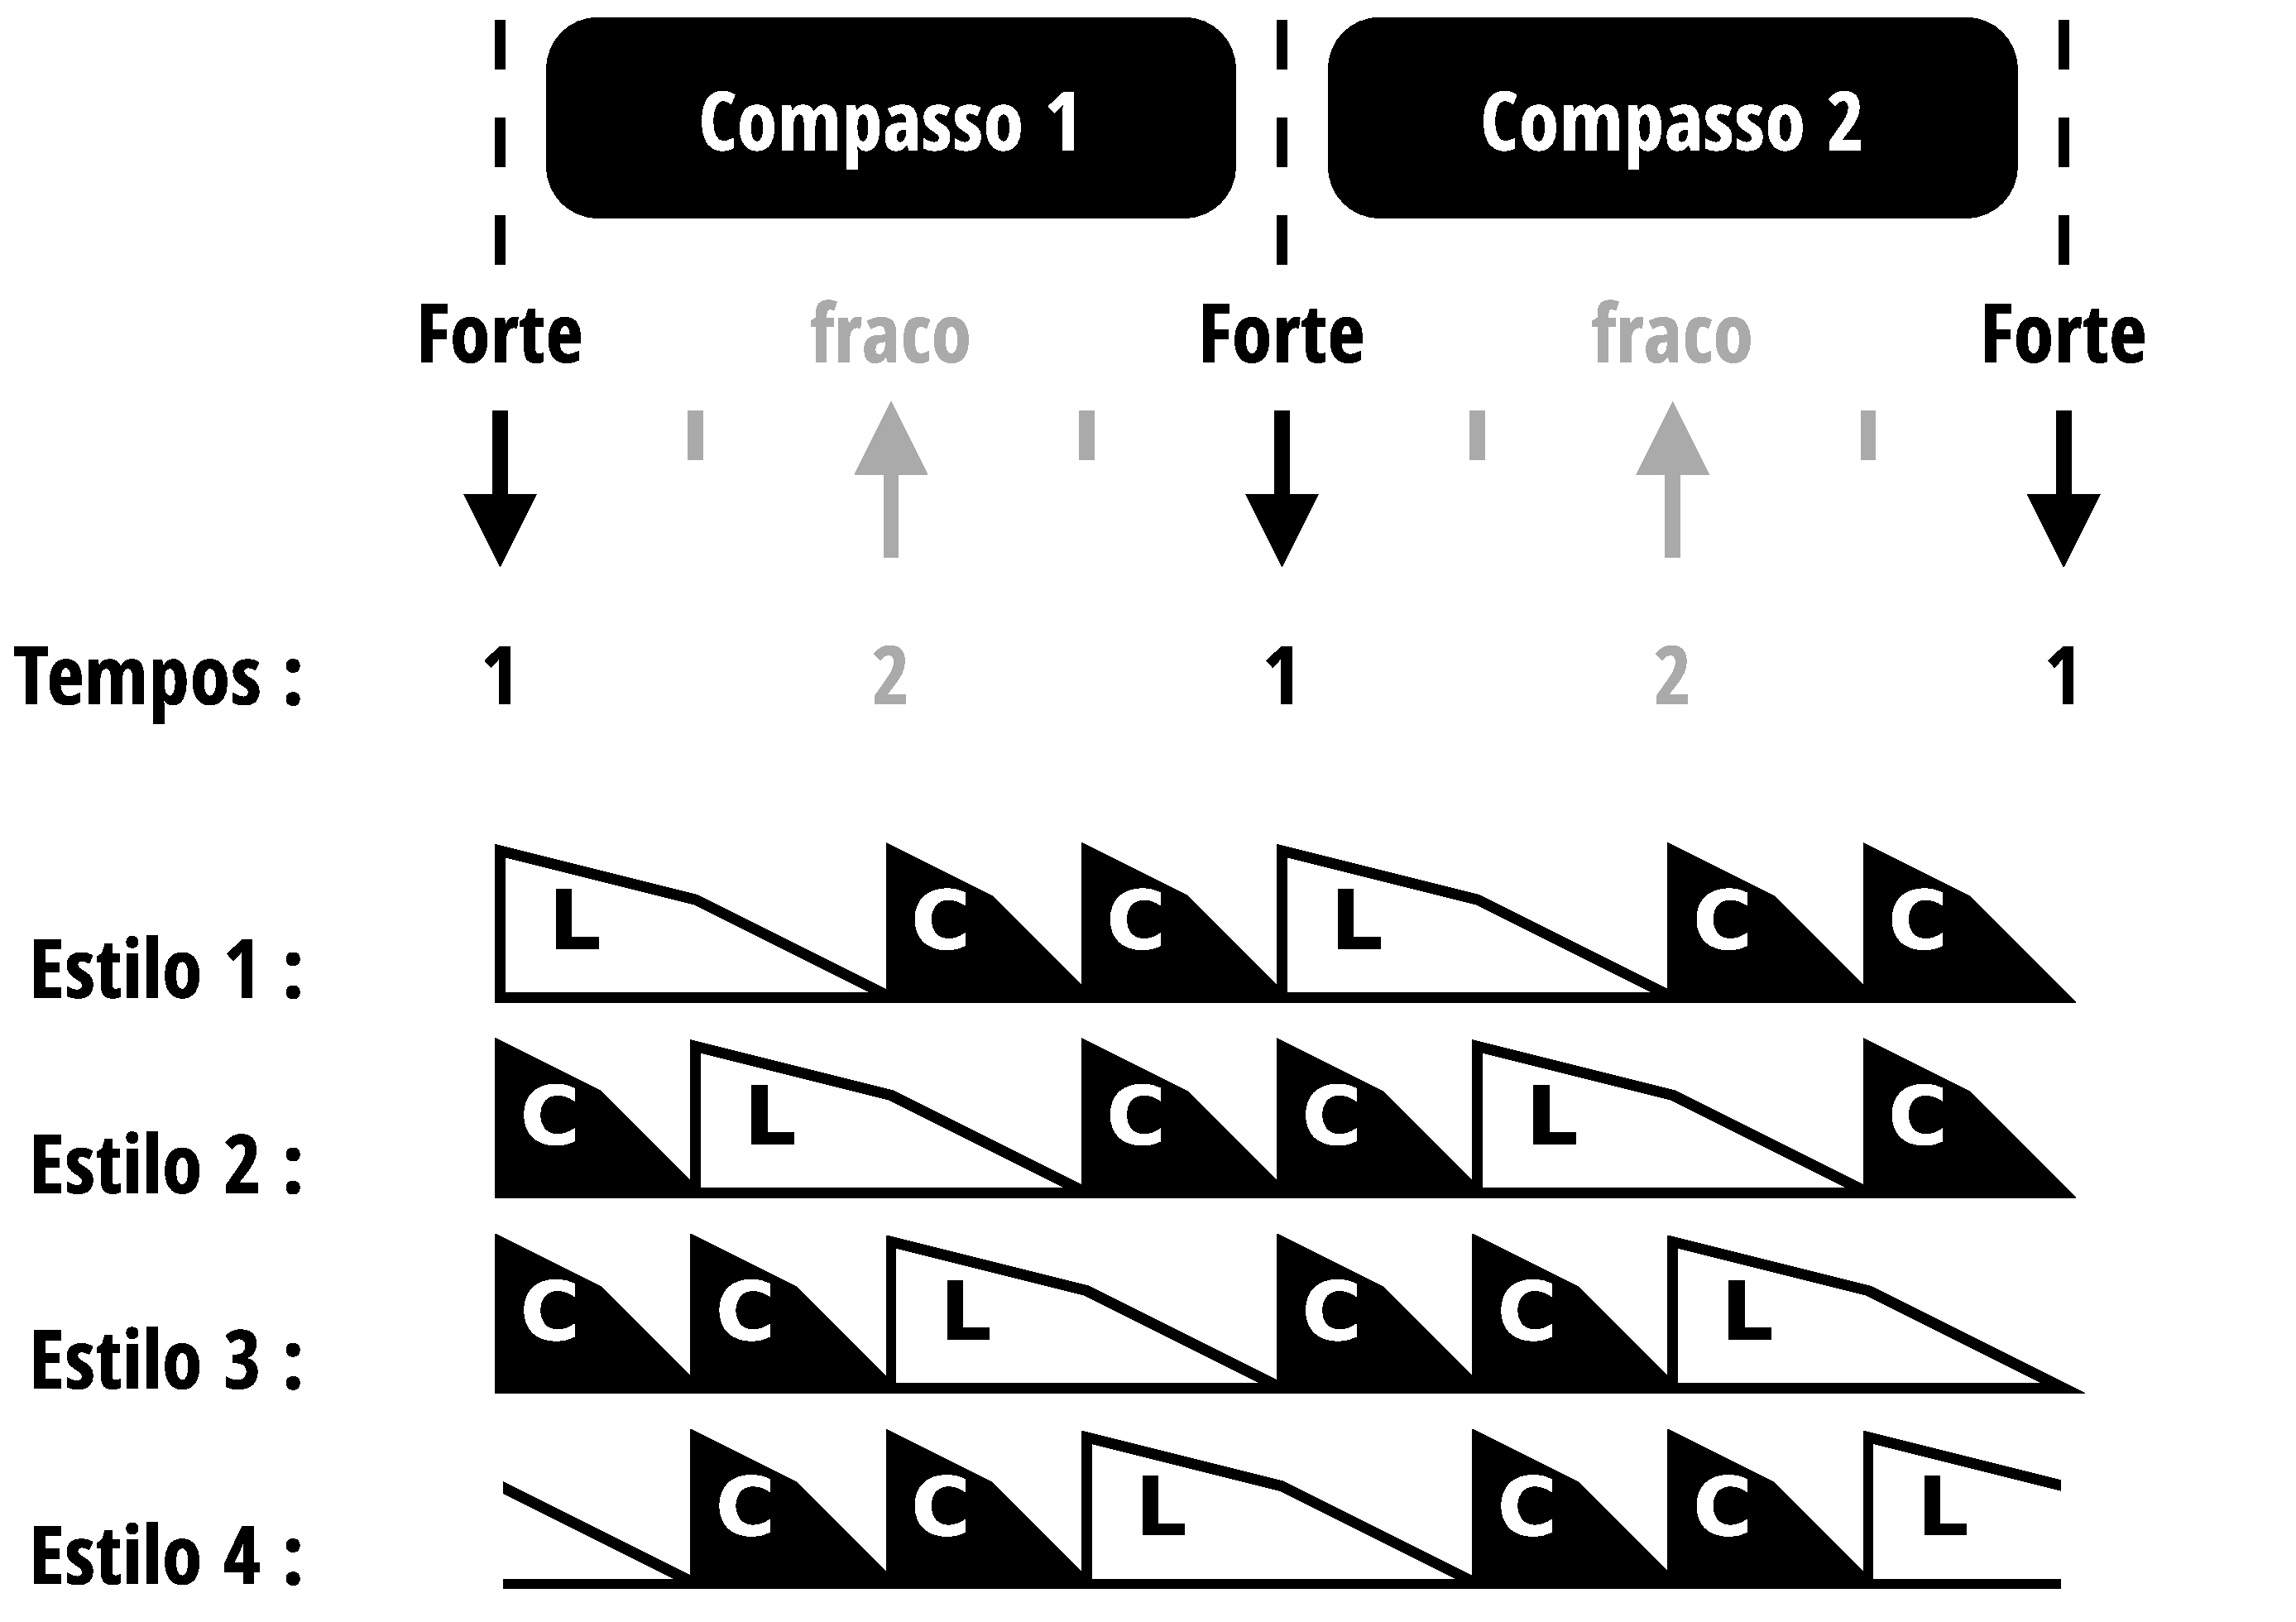
\includegraphics[width=0.75\textwidth]{chapters/cap-musicalidade/bailarcontratempo.eps}
    \caption{Dançando no tempo forte e em contra do tempo forte.}\label{fig:tempovscontratempo}
\end{figure}




%%%%%%%%%%%%%%%%%%%%%%%%%%%%%%%%%%%%%%%%%%%%%%%%%%%%%%%%%%%%%%%%%%%%%%%%%%%%%%%%
\subsection{Que significa dançar em contra do tempo forte?}
\index{Dançar em contra do tempo forte}
Nesta seção é proposta uma definição para ``dançar em contra do tempo forte''  
ou ``dançar a contratempo'',
 sendo o uso do termo contratempo uma ``metáfora'' na dança do mesmo termo na música;
assim, esta terá uma afinidade  com os usos explicados nas 
Seções \ref{subsec:contratempoespanha} e \ref{subsec:contratempocuba},
e divergirá do uso mencionado na Seção \ref{subsec:contratempobrasil},
com o fim de ter uma coerência maior com a acepção musical do termo 
\hyperref[sec:contratempo]{\textbf{contratempo}}.
A explicação já foi adiantada\footnote{Para 
ver a definição de dançar em contra do tempo forte ir a Pag. \pageref{def:DancaNoContratempo}.}
 na Definição \ref{def:DancaNoContratempo};
onde se menciona que para dançar em contra do tempo forte deve-se primeiro definir,
 qual é o movimento principal ou inicial do passo,
e logo executar esse movimento ao inicio de qualquer tempo fraco, ou parte fraca do tempo.

\begin{example}[Frente trás:]
Seguindo a definição do movimento descrita no Exemplo \ref{ex:frentetrasex},
sabe-se que o movimento longo é o principal;
assim, para dançar em contra do tempo forte, esse movimento deve ser encaixado num tempo fraco,
ou parte fraca do tempo.
Isto é mostrado nos Estilos 2, 3 e 4 da Figura \ref{fig:tempovscontratempo},
onde ``L'' representa o movimento com deslocamento longo,
e ``C'' representa o movimento sem deslocamento.
\begin{itemize} 
\item No ``Estilo 2'' o passo é executado na parte fraca do tempo forte.
\item No ``Estilo 3'' o passo é executado no tempo fraco.
\item No ``Estilo 4'' o passo é executado na parte fraca do tempo fraco.
\end{itemize}
\end{example}
%%%%%%%%%%%%%%%%%%%%%%%%%%%%%%%%%%%%%%%%%%%%%%%%%%%%%%%%%%%%%%%%%%%%%%%%%%%%%%%%
\subsection{Mudar entre dançar no tempo forte e em contra do tempo forte}
Se percebemos  que estamos dançando em contra do tempo forte e desejamos dançar a favor do tempo forte,
podemos seguir as seguintes indicações para mudar o estilo de dança.
\begin{itemize}
\item Podemos executar um \hyperref[def:PassoAContratempo]{\textbf{passo a contratempo}}\footnote{ Para 
ver a definição de passo a contratempo ir a Pag. \pageref{def:PassoAContratempo}.},
o que provocará mudar nossa dança de dançar no tempo forte a dançar em contra do tempo forte.
\begin{example}[Passos a contratempo:]
\begin{inparaitem}
\item Caminhada a contratempo.
\end{inparaitem}
\end{example}
\item Quando realizamos um movimento, interrompemos ele num tempo fraco 
para iniciar o próximo num tempo forte.
\begin{example}
\begin{inparaitem}
\item Fazemos balaços um número impar de vezes.
\end{inparaitem}
\end{example}
\end{itemize}





\newpage
%%%%%%%%%%%%%%%%%%%%%%%%%%%%%%%%%%%%%%%%%%%%%%%%%%%%%%%%%%%%%%%%%%%%%%%%%%%%%%%%
%%%%%%%%%%%%%%%%%%%%%%%%%%%%%%%%%%%%%%%%%%%%%%%%%%%%%%%%%%%%%%%%%%%%%%%%%%%%%%%%
\section{Dançando fora do ritmo ou da métrica?}
\index{Musicalidade!Fora do ritmo}
\index{Musicalidade!Fora da métrica}

Existe uma confusão no uso da expressão ``dançar fora do ritmo'',
pois comumente é usado para se referir a ``dançar fora da métrica'';
é claro que um \hyperref[sec:pos:Ritmo]{\textbf{ritmo}} está sujeito a uma \hyperref[def:Metrica]{\textbf{métrica}}, 
e se falamos que estamos fora do ritmo,
podemos também nos estar referindo a  dançar fora da métrica, 
porém isto é uma imprecisão que poucas vesses conseguirá
uma correta transmissão de nossas ideias.
Para entender melhor esta diferença descreveremos ambos casos


\begin{definition}[Dançar fora da métrica]
Significa que, dada uma porção de peça musical,
nossos movimentos estão sendo executados sem 
\hyperref[sec:musicalidadeinfmutua]{\textbf{informação mutua}} com a \hyperref[def:Metrica]{\textbf{métrica}}
dessa porção de música.

A métrica de uma porção de música nos dá informação da distribuição
dos tempos dos compassos e também qual será o acento métrico de cada um desses tempos.
\end{definition}

\begin{definition}[Dançar fora do ritmo]
\label{def:fora-do-ritmo}
Significa que dada uma voz dentro de uma porção de peça musical,
nossos movimentos estão sendo executados sem 
\hyperref[sec:musicalidadeinfmutua]{\textbf{informação mutua}} com a 
informação \hyperref[sec:pos:Ritmo]{\textbf{rítmica}} dessa voz nessa porção de música.

O ritmo de uma voz na música, 
se refere à distribuição temporal na execução dos sons e a sua proporção na duração
destes.
\end{definition}

Para entender melhor a Definição \ref{def:fora-do-ritmo}, a 
Figura \ref{fig:fora-do-ritmo-0-1} mostra a pauta de uma melodia executada por um bandolim, 
representando a voz escolhida para nossa dança; 
na parte inferior da pauta está representada a parte rítmica dessa melodia.
Assim, nesse caso, dançar fora do ritmo implica dançar fora do ritmo do bandolim;
é dizer, que entre esse ritmo e nossa dança existe pouca ou nula informação mutua.
Pelo que se acompanhamos essa melodia executando um ritmo regular como 
\Vier \Acht \Acht~(tum tic tic), com o tum no tempo forte;
nos dançaríamos dentro da métrica da melodia,
mas fora do ritmo dela. 
Assim, a frase ``dançar fora da métrica'' é a que expressa melhor o fato de estar descompromissado com os tempos
e os acentos nos compassos. 
\begin{figure}[!h]
    \centering 
    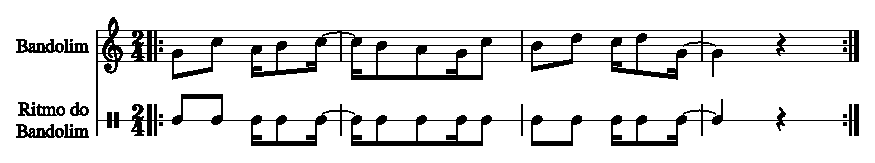
\includegraphics[width=0.99\textwidth]{chapters/cap-musicalidade/fora-do-ritmo-0-1.eps}
    \caption{Dançando respeitando a métrica.}
    \label{fig:fora-do-ritmo-0-1}
\end{figure}

\begin{example}[Dançando dentro da métrica:]
A Figura \ref{fig:fora-do-ritmo-com} mostra três casos onde um dançarino
executa bases rítmicas dentro da métrica da música. 
Neste caso a música  tem um \hyperref[subsec:compassobinario]{\textbf{compasso binário simples}}.
\begin{itemize}
\item Na primeira base rítmica se utiliza um ritmo repetitivo e regular \Vier \Acht \Acht~(tum tic tic),
com o mesmo período e acentuação estabelecido pela métrica. 
\item A segunda base rítmica, ao igual que a primeira, cumpre a métrica da música,
só que agora usa um ritmo \Vier \Vier~(tum tum).
\item A terceira base rítmica, ao igual que as anteriores, cumpre a métrica da música,
só que agora usa um ritmo \Acht. \Sech \Vier~(bum a tum).
\end{itemize}
\end{example}

\begin{figure}[!h]
    \centering 
    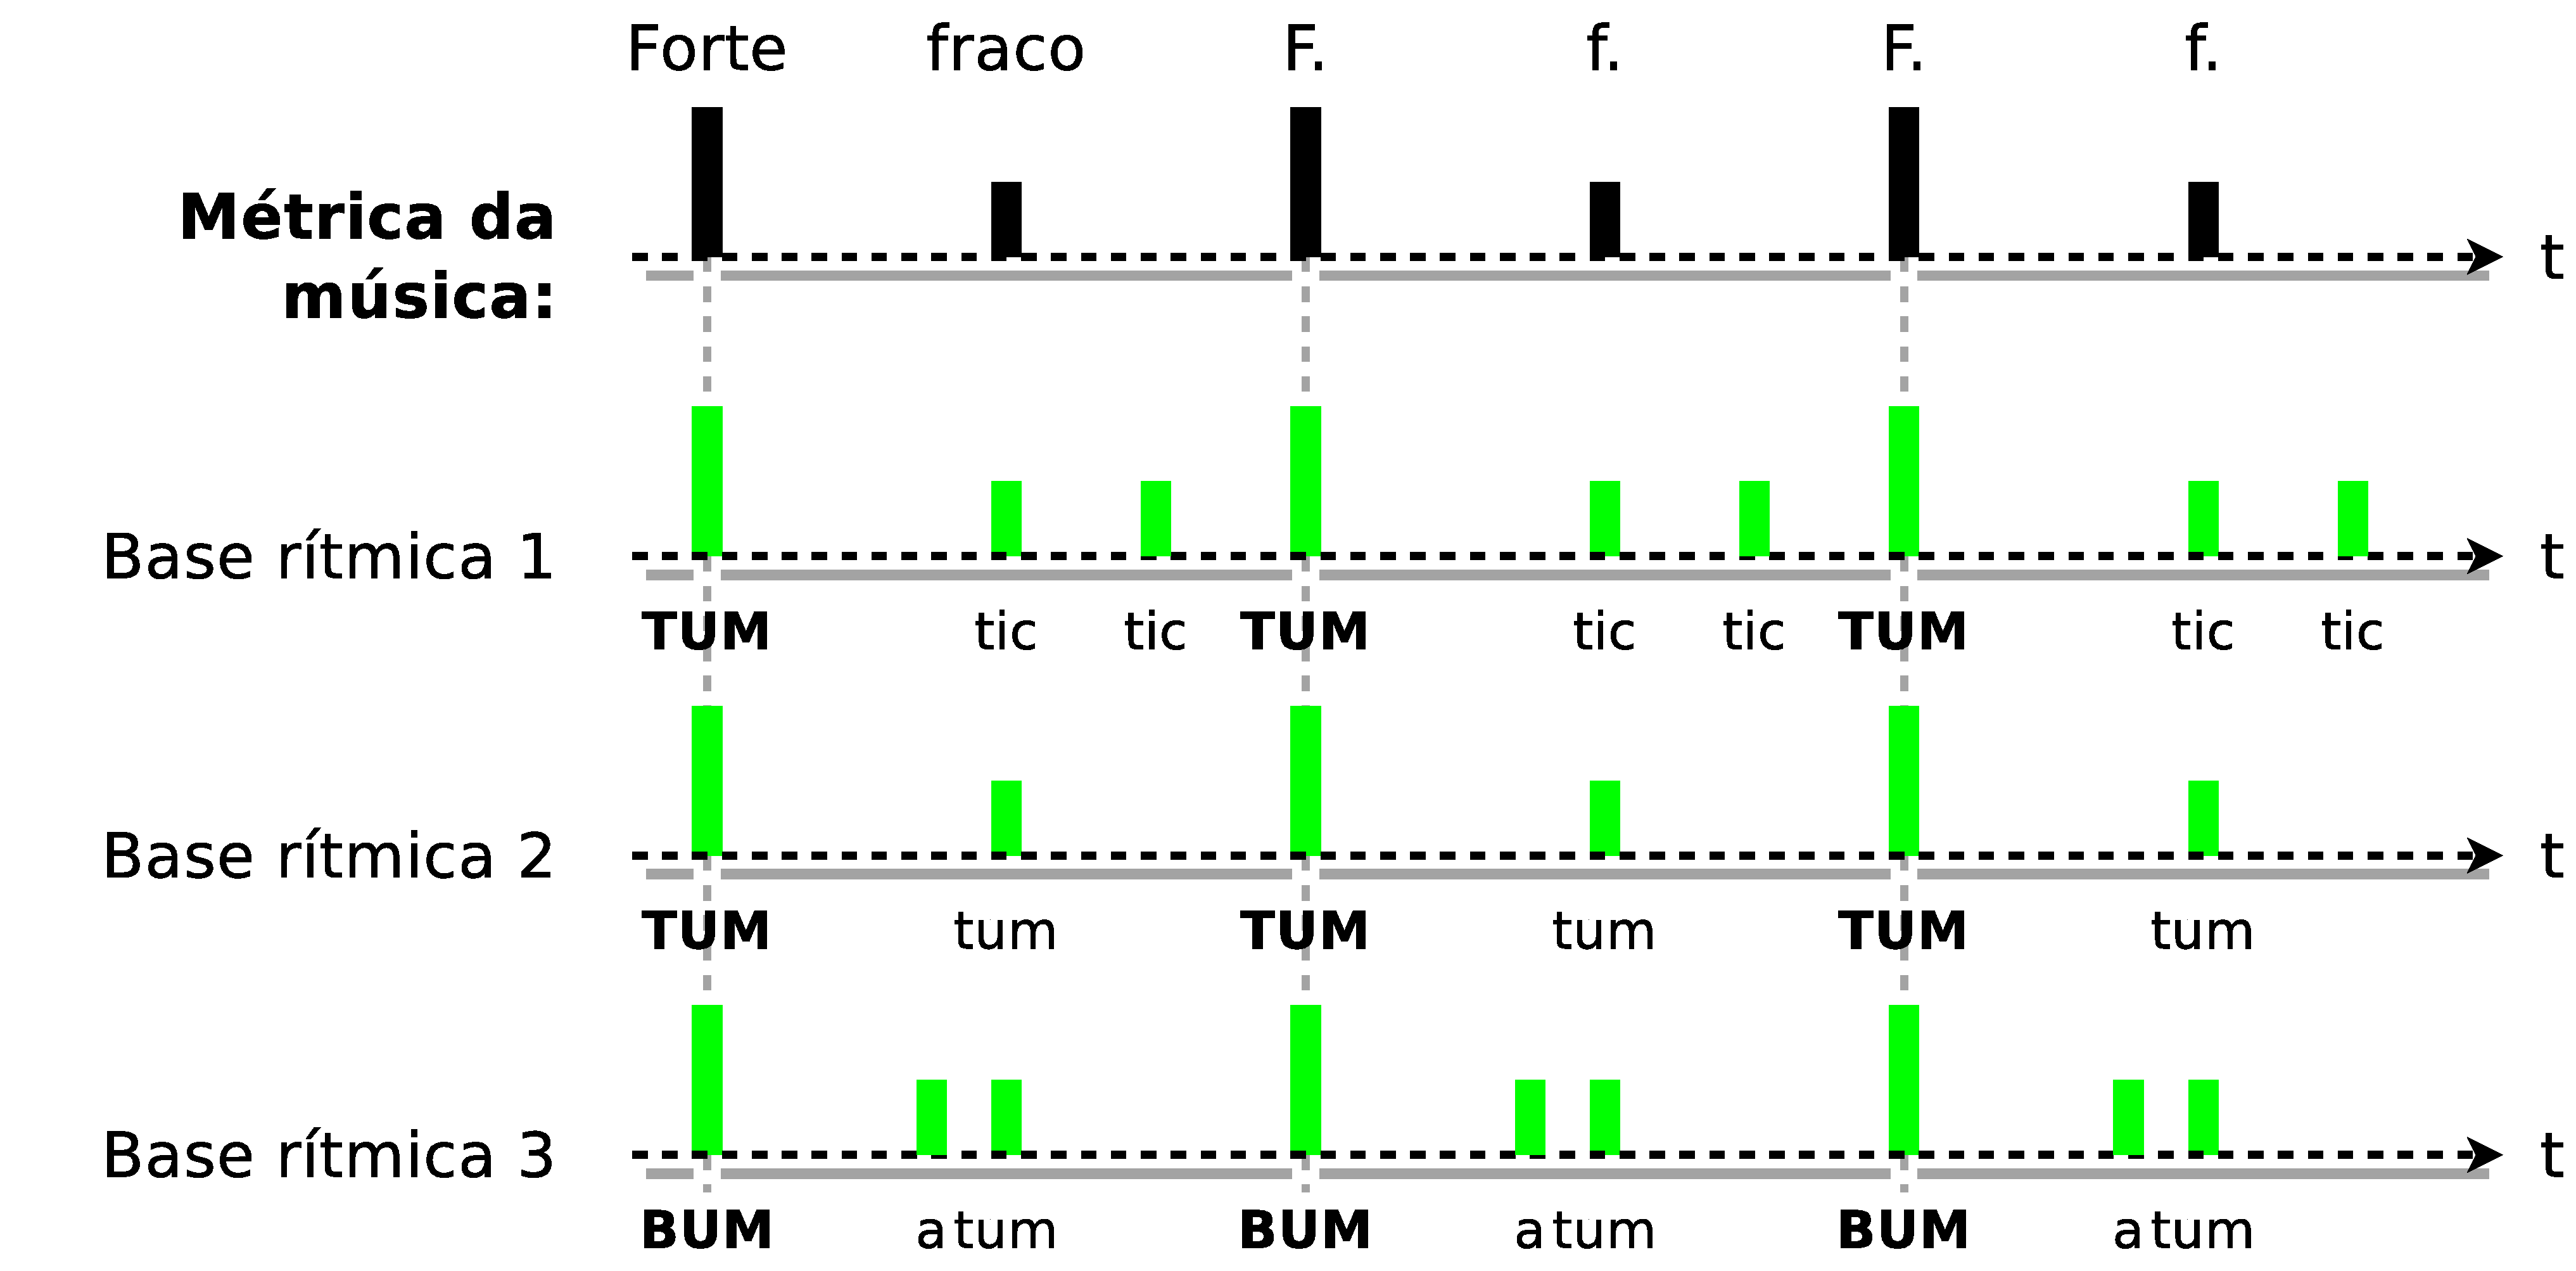
\includegraphics[width=0.89\textwidth]{chapters/cap-musicalidade/fora-do-ritmo-com.eps}
    \caption{Dançando respeitando a métrica.}
    \label{fig:fora-do-ritmo-com}
\end{figure}

\begin{tcbattention}
\begin{itemize}
\item Mais detalhes sobre como \hyperref[subsec:perceberTF1]{\textbf{reconhecer os tempos fortes}} 
e fracos podem ser vistos na Seção \ref{subsec:perceberTF1}.
\item Mais detalhes sobre o que é \hyperref[subsec:dancametrica]{\textbf{dançar na métrica}}, 
podem ser vistos na Seção \ref{subsec:dancametrica}.
\item Mais detalhes sobre o que é \hyperref[subsec:dancaritmo]{\textbf{dançar no ritmo}}, 
podem ser vistos na Seção \ref{subsec:dancaritmo}.
\item Outros temas relativos a dançar no ritmo são: 
\hyperref[subsec:dancamelodia]{\textbf{dançar na melodia}} e
\hyperref[subsec:dancamusica]{\textbf{dançar na música}},
que podem ser vistos nas Seções \ref{subsec:dancamelodia} e \ref{subsec:dancamusica},
respetivamente.
\end{itemize}
\end{tcbattention}

\begin{example}[Dançando fora da métrica:]
\label{ex:fora-do-ritmo:2}
A Figura \ref{fig:fora-do-ritmo-sem} mostra três casos 
onde um dançarino executa bases rítmicas fora da métrica da música,
Neste caso as três bases rítmicas utilizam um ritmo repetitivo e regular \Vier \Acht \Acht~(tum tic tic),
e a música  tem um \hyperref[subsec:compassobinario]{\textbf{compasso binário simples}}.
\begin{itemize}
\item A primeira base rítmica é executada com um \hyperref[sec:Andamento]{\textbf{andamento}} com
a mesma velocidade que a métrica da música; 
porém os movimentos tem uma desfasagem (atraso) na acentuação. 
Muito provavelmente produzido porque o dançarino esperou sentir o pulso musical para logo atuar,
e não predizer lho e atuar. 
\item A segunda base rítmica também é executada com um \hyperref[sec:Andamento]{\textbf{andamento}} com
a mesma velocidade que a métrica da música; 
porém os movimentos são acentuados em lugares aleatórios, 
pelo que não se está acompanhando a acentuação métrica.
\item A terceira base rítmica é executada com um \hyperref[sec:Andamento]{\textbf{andamento}} incorreto;
assim, mesmo que ele acentue seus passos de forma regular, estes sempre estarão mal colocados,
produto da desfasagem provocada pelas diferentes velocidades de andamento,
neste caso o dançarino tem um andamento de maior velocidade.
\end{itemize}
\end{example}
\begin{figure}[!h]
    \centering 
    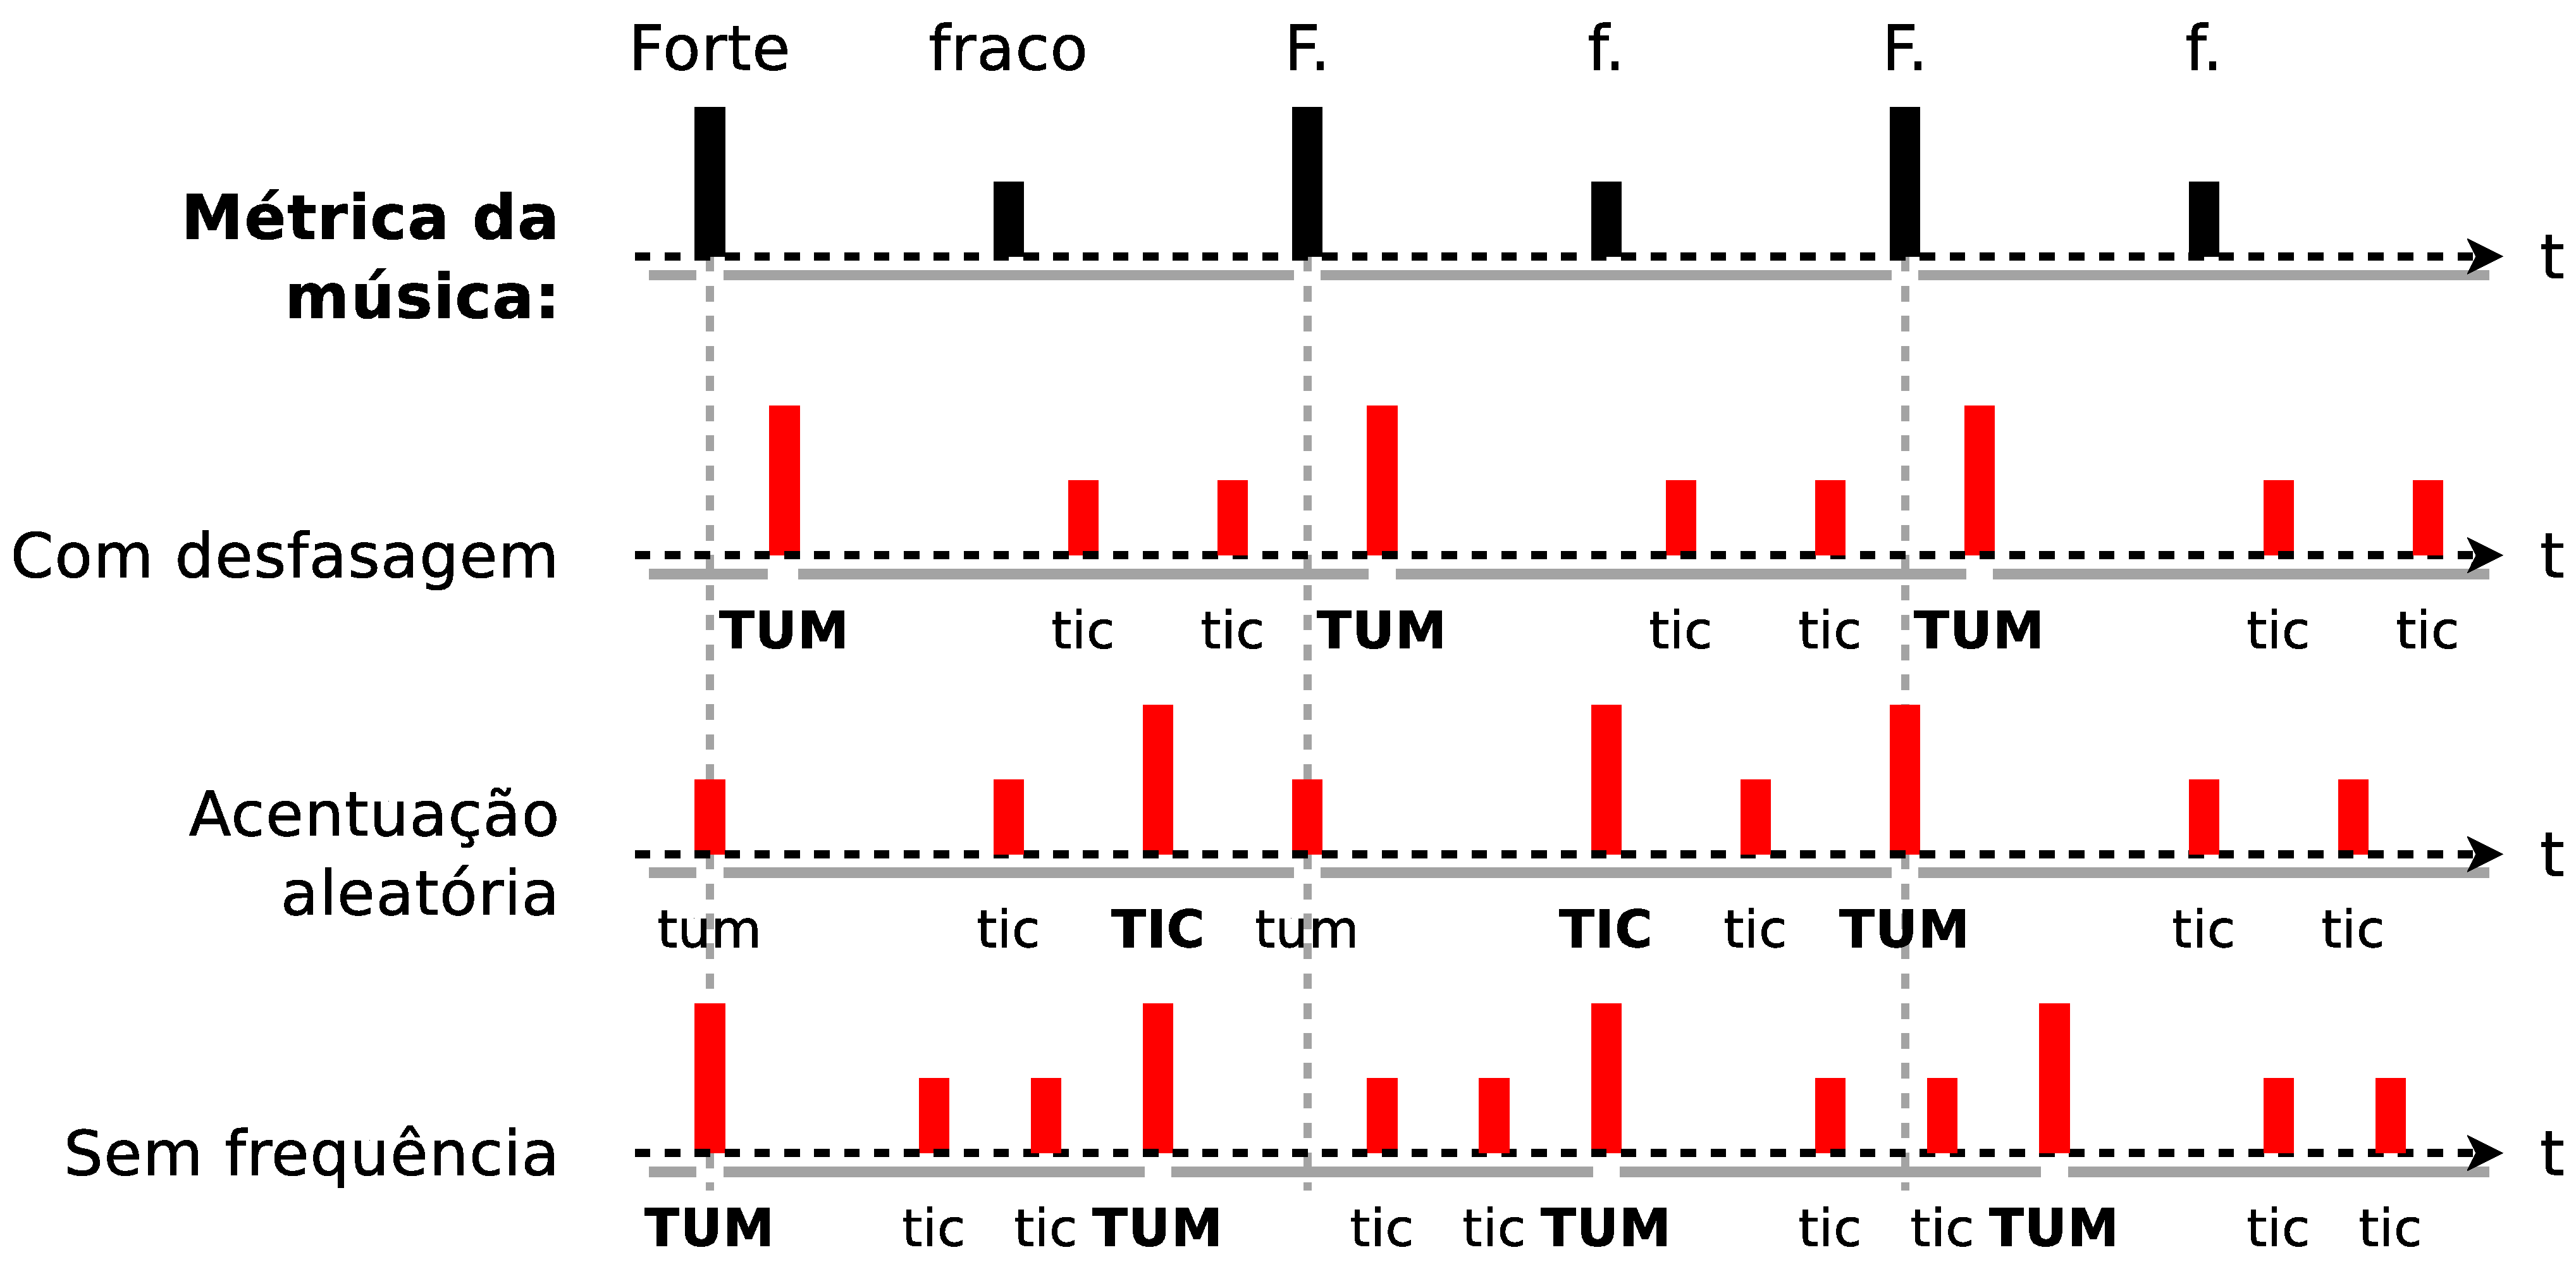
\includegraphics[width=0.89\textwidth]{chapters/cap-musicalidade/fora-do-ritmo-sem.eps}
    \caption{Dançando fora da métrica.}
    \label{fig:fora-do-ritmo-sem}
\end{figure}

Devemos ressaltar do Exemplo \ref{ex:fora-do-ritmo:2} que,
da mesma forma que na música, acentuar fora do acento métrico não é considerado um erro e sim um adorno; 
dançar não respeitando a acentuação métrica não necessariamente é considerado um erro,
e sim um enfeite. Mas, esta característica deve estar sobre o controle do dançarino,
e não ser algo solto à arbitrariedade, 
pois se nossa acentuação na dança tem pouca 
\hyperref[sec:musicalidadeinfmutua]{\textbf{informação mutua}} com o que está acontecendo na música, 
provavelmente o produto final (a dança) se perceberá com pouca musicalidade.  


